\documentclass[12pt,a4paper]{article}

\usepackage{graphicx}                            % Para poder incluir gráficos.
\usepackage[brazilian]{babel}                    % Para separar as sílabas, e colocar os nomes padrão (capítulo, bibliografia, etc.) em português.
\usepackage[utf8]{inputenc}                      % Para poder escrever diretamente com acentos, sem ter que usar códigos.
\usepackage[T1]{fontenc}                         % Para poder copiar do PDF acentos.
\usepackage{natbib}                              % \citep{jon90} --> (Jones et al., 1990)
\usepackage[colorlinks,citecolor=blue]{hyperref} % Para colocar links nas referências, equações, figuras, etc, além de menu árvore no PDF.
\usepackage{verbatim}                            % Para poder comentar regiões do arquivo .tex 
\usepackage[footnotesize,bf]{caption}                   % Para que legendas de figuras e tabelas fique em fonte menor e com negrito.
\usepackage{amssymb}                             % Para poder utilizar alguns símbolos matemáticos especiais.
\usepackage{amsmath}                             % Para poder usar o comando 'cases', e possivelmente outros.
\usepackage{fancyhdr}                            % Para poder fazer cabeçalhos e rodapés mais bonitos.
%\usepackage{epstopdf}                            % Para poder usar imagens .eps no compilador pdflatex (que permite usar imagens .png).
\usepackage{times}                               % Para usar typeset bem definido.
\usepackage{titlesec}                            % Para poder redefinir o formato dos títulos de seções
\usepackage[svgnames]{xcolor}                    % Várias cores (+150)                         
\usepackage{helvet}                              % Fonte helvética
\usepackage{lipsum}                              % Para preencher com texto. 
\usepackage{booktabs}                            % Para usar toprule, etc. que vem das tabelas do pandas.
\usepackage{longtable}                           % Para quebrar tabelas
\usepackage{float}                               % Para poder usar figure placement H.
\usepackage{authblk}

% Cores dos hyperlinks do texto:
\hypersetup{
     %colorlinks = blue,
     linkcolor = DarkRed,
     %anchorcolor = yellow,
     %citecolor = cyan,
     %urlcolor  = magenta
     }

% Para poder se referir ao título das sub-seções no header:
\let\Chaptermark\chaptermark
\def\chaptermark#1{\def\Chaptername{#1}\Chaptermark{#1}}
\let\Sectionmark\sectionmark
\def\sectionmark#1{\def\Sectionname{#1}\Sectionmark{#1}}
\let\Subsectionmark\subsectionmark
\def\subsectionmark#1{\def\Subsectionname{#1}\Subsectionmark{#1}}
\let\Subsubsectionmark\subsubsectionmark
\def\subsubsectionmark#1{\def\Subsubsectionname{#1}\Subsubsectionmark{#1}}


%%% Formatting %%%
% Cores:
\definecolor{MSBlue}{rgb}{.204,.353,.541}
\definecolor{MSLightBlue}{rgb}{.31,.506,.741}
\newcommand{\secColor}{\color{RoyalBlue}}
% Título das seções:
\titleformat*{\section}{\LARGE\bfseries\sffamily\secColor}
\titleformat*{\subsection}{\Large\bfseries\sffamily\secColor}
\titleformat*{\subsubsection}{\normalsize\bfseries\sffamily\secColor}
\renewcommand{\headrule}{\secColor\hrule}
% Header:
\pagestyle{fancy}
\setlength\headheight{26pt} %% just to make warning go away. Adjust the value after looking into the warning.
%\fancyhead[L]{\fontsize{10}{12}\sffamily\secColor\rightmark}
\fancyhf{}
\fancyhead[L]{\fontsize{10}{12}\sffamily\secColor\thesubsection. \Subsectionname}
\rhead{
\includegraphics[width=3cm]{acredito_fundobranco.png}}
\fancyfoot[C]{\thepage}
% Para quando não tem sub-seção:
\fancypagestyle{final}{
    \fancyhead[L]{\fontsize{10}{12}\sffamily\secColor\rightmark}
\rhead{
\includegraphics[width=3cm]{acredito_fundobranco.png}}
}

% My commands
\newcommand{\tinyurl}[1]{{\tiny\url{#1}}}
\newcommand{\footurl}[1]{{\scriptsize\url{#1}}}
\newcommand{\HX}[1]{{\centering\color{red}\large<#1>}}

\author{Henrique S. Xavier \& João Carabetta}
\title{\secColor\Huge\sffamily\bfseries 100 dias de congresso\\\texttt{<em dados>}}
\affil{Gabinete compartilhado\\Movimento Acredito no Congresso Nacional}


%%%%%%%%%%%%%%%% REPORT %%%%%%%%%%%%%%%%%%
\begin{document}

% Página de rosto:
\pagenumbering{gobble}
\thispagestyle{empty}
\maketitle
%\tableofcontents
\pagebreak

\thispagestyle{empty}
\tableofcontents
\pagebreak

% Relatório mesmo:
\thispagestyle{plain}
\pagenumbering{arabic}

\setcounter{secnumdepth}{0}
\section{Agradecimentos}

Agradecemos às seguintes pessoas que nos enviaram
comentários e sugestões quanto à nossa análise e relatório: Prof. Dr. Robert Bonifácio, professor adjunto de ciência política da Universidade Federal de Goiás (UFG); e Dr. Ana Carla Abrão Costa, da consultoria Oliver Wyman. Dado o tempo exíguo para a preparação deste relatório, diversas sugestões não puderam ser implementadas mas serão incorporadas em futuras análises.  


%%%%%%%%%%%%%%%%%%%
\setcounter{secnumdepth}{3}
\section{Introdução}
\label{sec:intro}

Este trabalho visa apresentar um panorama do congresso nacional brasileiro nos 100 primeiros dias da $56^{\mathrm{\underline{a}}}$ legislatura, que
se iniciou no dia 1 de fevereiro de 2019, utilizando as bases de dados abertos da câmara\footnote{\footurl{http://dadosabertos.camara.leg.br/}}
e do senado\footnote{\footurl{http://www12.senado.leg.br/dados-abertos}}. Além de apresentar o cenário atual, também buscamos analisar
as características históricas do congresso, tanto para fins de comparação quanto de construção de um retrato de suas características
mais estruturais. Os objetivos deste relatório são dois: de servir de subsídio para a atividade parlamentar do movimento Acredito na
câmara e no senado, e de prover à sociedade mais informações relativas ao trabalho de seus representantes e das estruturas governamentais
utilizadas nessa representação. Este último objetivo atende, na prática, ao valor de transparência do movimento Acredito.

Dado o curto período de tempo disponível para a realização deste estudo, apresentamos aqui uma análise inicial que
certamente poderá ser desdobrada e aprofundada em investigações futuras. Essa análise foi segmentada em duas frentes,
uma focada nos parlamentares e outra nas proposições -- e.g. projetos de lei (PLs), medidas provisórias (MPs) e propostas
de emenda à constituição (PECs) -- em tramitação.

Em relação aos parlamentares, buscamos investigar:
(\emph{i}) o alinhamento ao governo e a fidelidade partidária;
(\emph{ii}) e o nível de participação e engajamento;
(\emph{iii}) a distribuição de cargos e poder;
e (\emph{iv}) o uso da cota parlamentar (verba destinada a cobrir os custos do trabalho parlamentar). 
Em relação às proposições, analisamos quais temas são os mais recorrentes historicamente e na atual legislatura.

\subsection{Dados faltantes}
\label{sec:dados-faltantes}

Um de nossos primeiros achados se refere à limitação das bases de dados, particularmente em relação
aos dados mais recentes, o que impediu a análise completa dos últimos 100 dias. Dados listados
nas bases como disponíveis e seguindo atualização diária estão, em alguns casos, incompletos.
Nesses casos, optamos por apenas realizar uma análise histórica. Os casos de dados incompletos
encontrados são:

\begin{itemize}

\item \emph{Despesas com a cota parlamentar:} os deputados tem um prazo de 90 dias para solicitar reembolso
  à cota parlamentar\footnote{\footurl{https://www2.camara.leg.br/comunicacao/assessoria-de-imprensa/cota-parlamentar}}
  e empresas aéreas chegam a demorar mais do que isso para comunicar à câmara a emissão de
  bilhetes, o que torna incompleta a amostra de gastos dos últimos 100 dias. Esse não é um problema de publicação dos
  dados, e sim o tempo característico do processo de uso da cota parlamentar, de forma que ele não poderia ser contornado
  no futuro. Também foram identificados registros de dois anos atrás (2017) sendo atualizados neste ano (2019).   

\item \emph{Participação em órgãos (e.g. comissões):} embora estejam listadas no portal da
  câmara\footnote{\footurl{https://www2.camara.leg.br/deputados/pesquisa}}, em muitos casos as participações
  dos atuais deputados em comissões e na mesa diretora não aparecem nas bases de dados abertos. Isso
  impossibilita a coleta automatizada e rápida dos dados e inviabilizou a análise dessas participações para
  a legislatura atual. O fato dos dados aparecerem no portal da câmara mostra que esse é um problema de
  disponibilização que, provavelmente, pode ser resolvido facilmente.

\item \emph{Histórico das lideranças na câmara}: as bases de dados listam as atuais lideranças na câmara
  de blocos e partidos, mas não guardam o histórico. Embora ainda seja possível realizar uma análise desses 
  dados nos atuais 100 primeiros dias, não é possível construir um histórico para comparação. Ao menos para
  o futuro, esse parece um problema de simples resolução, uma vez que bastaria acumular os dados publicados
  diariamente.
  
\item \emph{Orientação Partidária}: Na Câmara, a orientação partidária em muitos casos é suprimida já que ela vem agregada por blocos partidários. Existem situações que a orientação é apresentada como \textit{'PsbPsdbPodemos...'}, de maneira que não é possível saber quais partidos foram suprimidos. No Senado, não existe orientação partidária.
\end{itemize}

\subsection{Principais achados}

Além da questão dos dados faltantes (Seção \ref{sec:dados-faltantes}), os principais achados
sobre os 100 primeiros dias do congresso são os seguintes:

\begin{itemize}

\item Os alinhamentos entre a orientação do governo e os votos na câmara dos deputados e no senado são significativos e
  comparáveis aos 100 primeiros dias dos governos anteriores (com exceção do segundo mandato de Dilma Rousseff,
  que destoa pela falta expressiva de apoio). Esse fato constrasta com as publicações em jornais e revistas
  de opinião que enfatizam a dificuldade do governo em articular com o congresso (veja a Seção \ref{sec:apoio-governo}, na qual também levantamos hipóteses para explicar essa aparente diferença de cenário).

\item Os temas que ganharam destaque nos projetos de lei apresentados na câmara em 2019 são: meio ambiente e desenvolvimento
  sustentável; direito constitucional; direito penal e processual penal; e defesa e segurança
  (veja a Seção \ref{sec:temas-camara}). Os que ganharam
  destaque no senado são: meio ambiente; direitos humanos e minorias; datas comemorativas; e família, proteção a crianças,
  adolescentes, mulheres e idosos (Seção \ref{sec:temas-senado}). 
  Por serem objetos de projetos de lei, concluímos que os atuais parlamentares
  buscam alterar a legislação relacionada a esses temas. A pauta relacionada a meio ambiente de destaca com força
  em ambas as casas.

\item A atuação parlamentar via ações legislativas (e.g. apresentação de projetos de lei, pedidos de
audiência pública, relatoria de proposições) é altamente concentrada em poucos parlamentares, e diferentes tipos de ação são utilizados pela oposição e situação (Seção \ref{sec:atividade-parlamentar}).

\end{itemize}

\subsection{Análises históricas}

Dentre as investigações puramente históricas, ressaltamos os seguintes resultados como mais relevantes:
\begin{itemize}

    \item A participação dos deputados em comissões e na mesa diretora segue uma
    sazonalidade marcada ao longo da legislatura, com maior vigor nos segundos e terceiros anos de mandato e baixa no último. Além disso, as participações em uma
    dada comissão duram, de maneira geral, um ano (Seção \ref{sec:cargos-deputados}).

    \item No período analisado (de 2009 a 2017), as despesas dos deputados via cota parlamentar seguiram uma regularidade bastante forte, com um nível de gastos médio
    estável e sazonalidades bem marcadas em períodos de um e quatro anos (veja a Seção \ref{sec:cota-parlamentar}). Também mostramos na mesma seção que os
    maiores gastos através da cota são com divulgação da atividade parlamentar e passagens aéreas.
    
    
\end{itemize}


%%%%%%%%%%%%%%%%%%%%%%
\section{Parlamentares}


%%%%%%%%%%%%%%%%%%%%%%%%%%%%%%%%
\subsection{Alinhamento com o governo}
\label{sec:apoio-governo}

Podemos estimar o alinhamento dos parlamentares com o governo através da correlação entre os votos dos parlamentares e a orientação de voto
dada pelo governo. Para fins de comparação, realizamos esse estudo para os 100 primeiros dias da presente legislatura
e das legislaturas anteriores, desde 1999. Votações nas quais não existia orientação do governo foram ignoradas, assim como abstenções e ausências. Obstruções foram contabilizadas como votos contrários. 

No caso do senado, não existe na base de dados o registro da orientação dada pelo governo. Nesse caso, nós utilizamos o voto do líder do governo de cada época como proxy dessa orientação. 

\subsubsection{Câmara}
\label{sec:apoio-governo-camara}

A Fig. \ref{fig:apoio-governo-deputados} mostra a distribuição de deputados e deputadas em função do grau de
alinhamento com a orientação do governo, nos 100 primeiros dias de legislatura, desde 1999 até hoje.
Na maioria dos casos, é possível notar um grupo significativo de deputados que vota 90\% das vezes ou mais em acordo com o governo.
No caso de 1999 (início do segundo mandato de Fernando Henrique Cardoso), mais da metade dos deputados votaram
com o governo 100\% das vezes, levando a mediana a esse valor. No início do segundo mandato de Dilma Rousseff,
esse grupo se diluiu e o alinhamento dos deputados se tornou bastante disperso.

\begin{figure}[H]
\centering
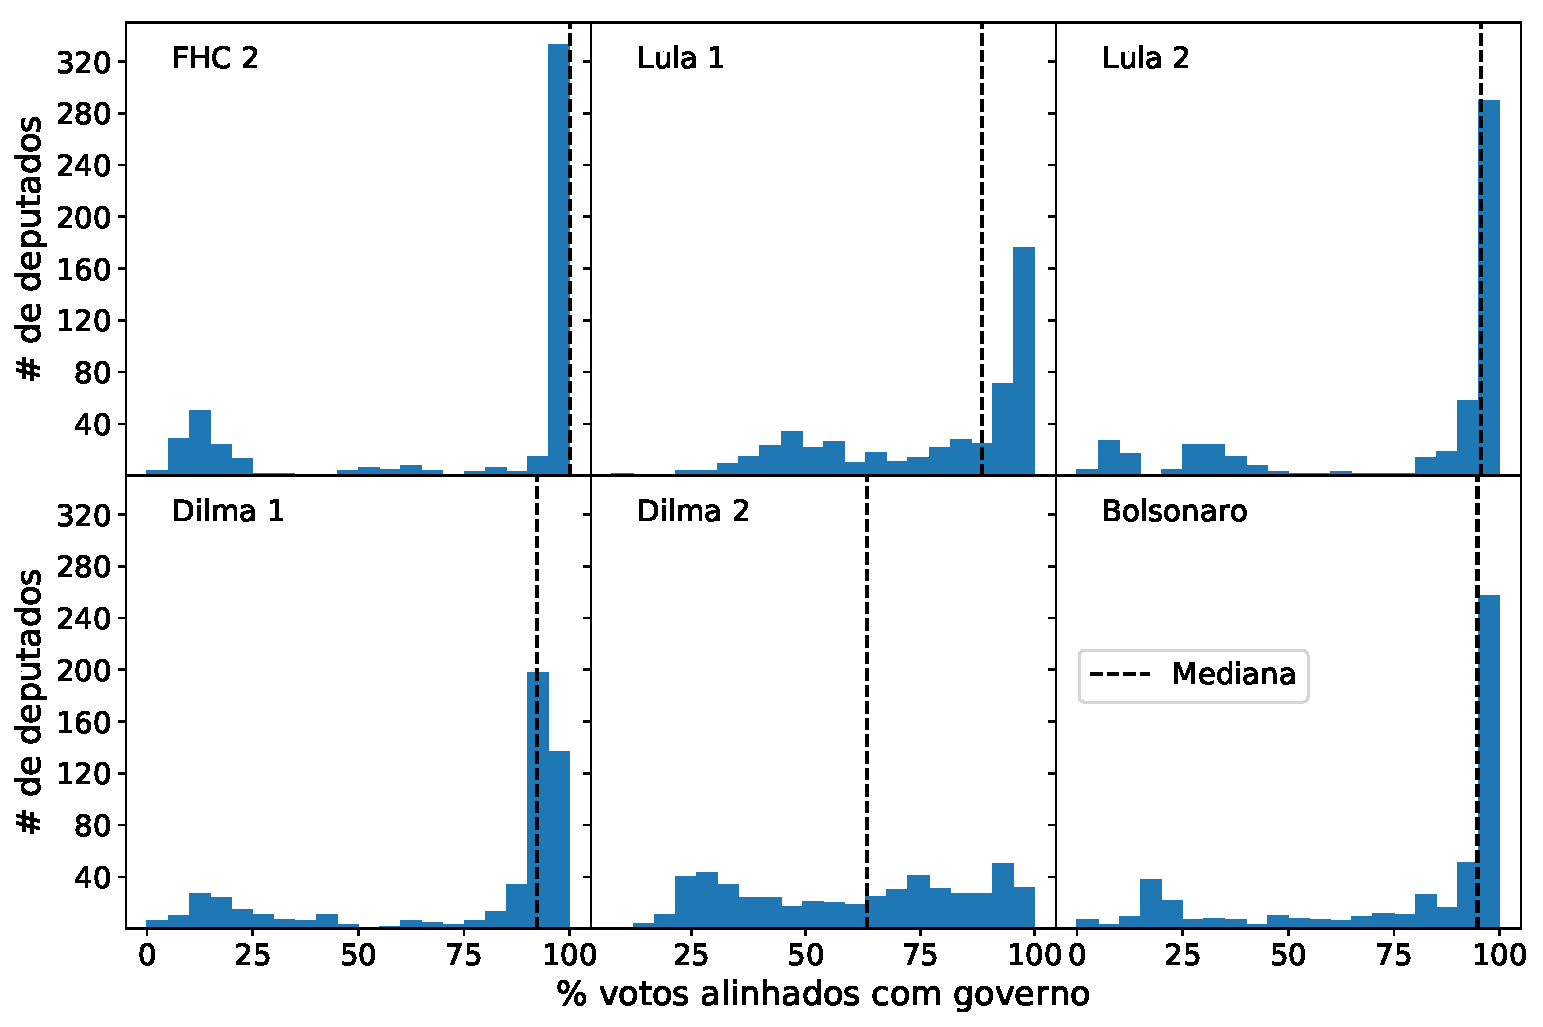
\includegraphics[width=1.0\textwidth]{graficos/apoio_ao_governo_deputados_2019-05-09.pdf}
\caption{Contagem do número de deputados em função da fração de seus votos no plenário que se
  alinham com a orientação do governo. Cada painel apresenta os dados dos 100 primeiros dias de
  cada legislatura, discriminadas pelo presidente da república no período. A linha vertical tracejada preta
  separa a metade dos deputados com maior e menor alinhamento.}
\label{fig:apoio-governo-deputados}
\end{figure}

Na maioria das legislaturas, a distribuição bimodal indica uma separação clara dos deputados
entre governo e oposição, sendo esta última contrária ao governo em mais de 2/3 das vezes.
Esse padrão se altera no primeiro mandato de Luiz Inácio Lula da Silva e no segundo mandato de Dilma.

A Fig. \ref{fig:apoio-governo-deputados} ainda indica que o governo de Jair Messias Bolsonaro está 
razoávelmente alinhado aos deputados, com distribuição similar à de governos anteriores. Esse dado contrasta
com a impressão derivada da cobertura da mídia, conforme mostra as manchetes da Fig. \ref{fig:manchetes-apoio}.
Uma hipótese para explicar essa aparente discrepância é que as manchetes em geral comentam sobre
a falta de articulação política no contexto da reforma da previdência, uma votação mais polêmica e
que exige um alinhamento maior (por se tratar de uma mudança na constituição). Outras hipóteses seriam
que a agenda de votações não está sendo comandada pelo governo, que a orientação do governo está seguindo os votos dos deputados ao invés de liderá-los, 
ou que a natureza das matérias enviadas ao congresso pelo presidente não inclui nada de polêmico ou relevante. Essa última hipótese pode afetar mais presidentes em primeiro mandato.

\begin{figure}[H]
  \centering
  %\fbox{
    %\begin{minipage}{\textwidth}
      \fbox{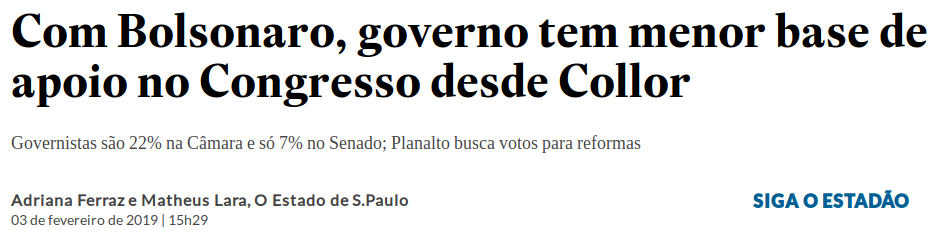
\includegraphics[width=1.0\textwidth]{manchetes/estadao-bolsonaro-menor-base.png}}
      \fbox{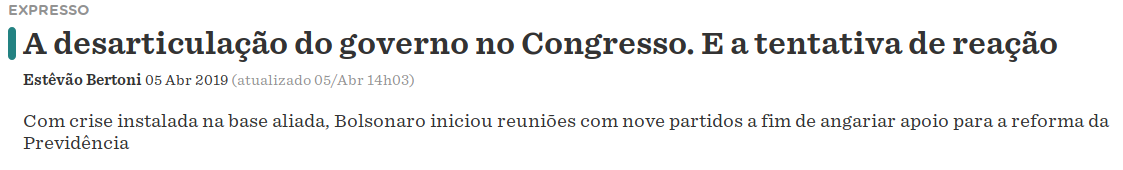
\includegraphics[width=1.0\textwidth]{manchetes/nexo-desarticulacao.png}}
      \fbox{
\includegraphics[width=1.0\textwidth]{manchetes/forum-PSL-ameaca-rebeliao.png}}
    %\end{minipage}
    %}
\caption[Exemplos de manchetes mencionando dificuldades do governo com o congresso, extraídas dos jornais
  O Estado de São Paulo e Nexo, e da Revista Fórum.]{Exemplos de manchetes mencionando dificuldades do governo com o congresso, extraídas dos jornais
  O Estado de São Paulo e Nexo, e da Revista Fórum.\footnotemark}
\label{fig:manchetes-apoio}
\end{figure}
\footnotetext{\\\tinyurl{http://politica.estadao.com.br/noticias/geral,com-bolsonaro-governo-tem-menor-base-de-apoio-no-congresso-desde-collor,70002706224}\\
  \tinyurl{http://www.nexojornal.com.br/expresso/2019/04/05/A-desarticula\%C3\%A7\%C3\%A3o-do-governo-no-Congresso.-E-a-tentativa-de-rea\%C3\%A7\%C3\%A3o}\\
  \tinyurl{https://www.revistaforum.com.br/parlamentares-do-psl-ameacam-rebeliao-contra-o-governo-jair-bolsonaro}}

Também analisamos o alinhamento ao governo por votação. A Fig. \ref{fig:apoio-governo-votacao} mostra o resultado
desse levantamento para os 100 primeiros dias das legislaturas desde 1999. Vemos que o segundo mandato
de Fernando Henrique obteve maioria absoluta (257 votos) em todas as votações dos 100 primeiros dias; já
o segundo mandato de Dilma é o único que não conseguiu que a média do número de votos por votação
superasse 257. Foi também nesse governo em que se registrou o maior número de votações em 100 dias.
O atual governo apresentou características típicas dos governos anteriores (com exceção do segundo mandato de Dilma), com alinhamento médio
acima da maioria absoluta e um número mais baixo de votações.

\begin{figure}[H]
\centering
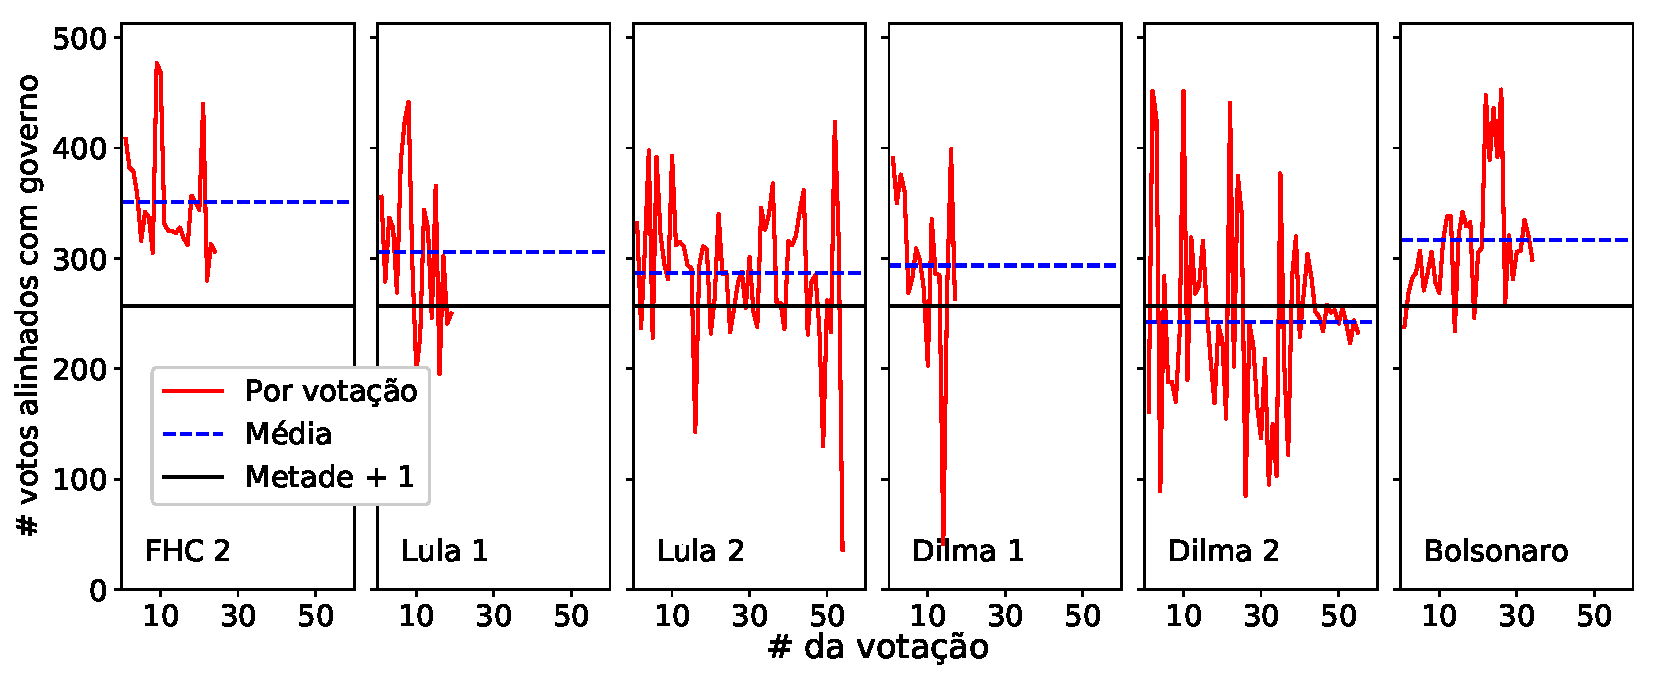
\includegraphics[width=1.0\textwidth]{graficos/apoio_ao_governo_por_votacao_2019-05-09.pdf}
\caption{Número de votos seguindo a orientação do governo, em cada votação dos 100 primeiros
  dias de congresso (em vermelho). Cada painel apresenta uma legislatura diferente, que teve
  um número diferente de votações nos 100 primeiros dias. A linha tracejada azul indica a média
  do número de votos obtidos em cada votação, e a linha contínua preta representa o mínimo de
  votos para se obter maioria absoluta (metade do total de deputados mais um).}
\label{fig:apoio-governo-votacao}
\end{figure} 

O alinhamento com o governo atual também foi estimado por partido: a Fig. \ref{fig:apoio-governo-partido} mostra ele atravessa múltiplos partidos, e que o grau de alinhamento com o governo varia de maneira
mais ou menos suave para a maioria dos partidos. Exceção a esse comportamento se dá com o PT, PSOL e
PCdoB, que formam uma oposição mais demarcada. A Fig. \ref{fig:apoio-governo-partido-G} apresenta os
mesmos dados mas apenas para os partidos com 10 deputados ou mais.

\begin{figure}[H]
\centering
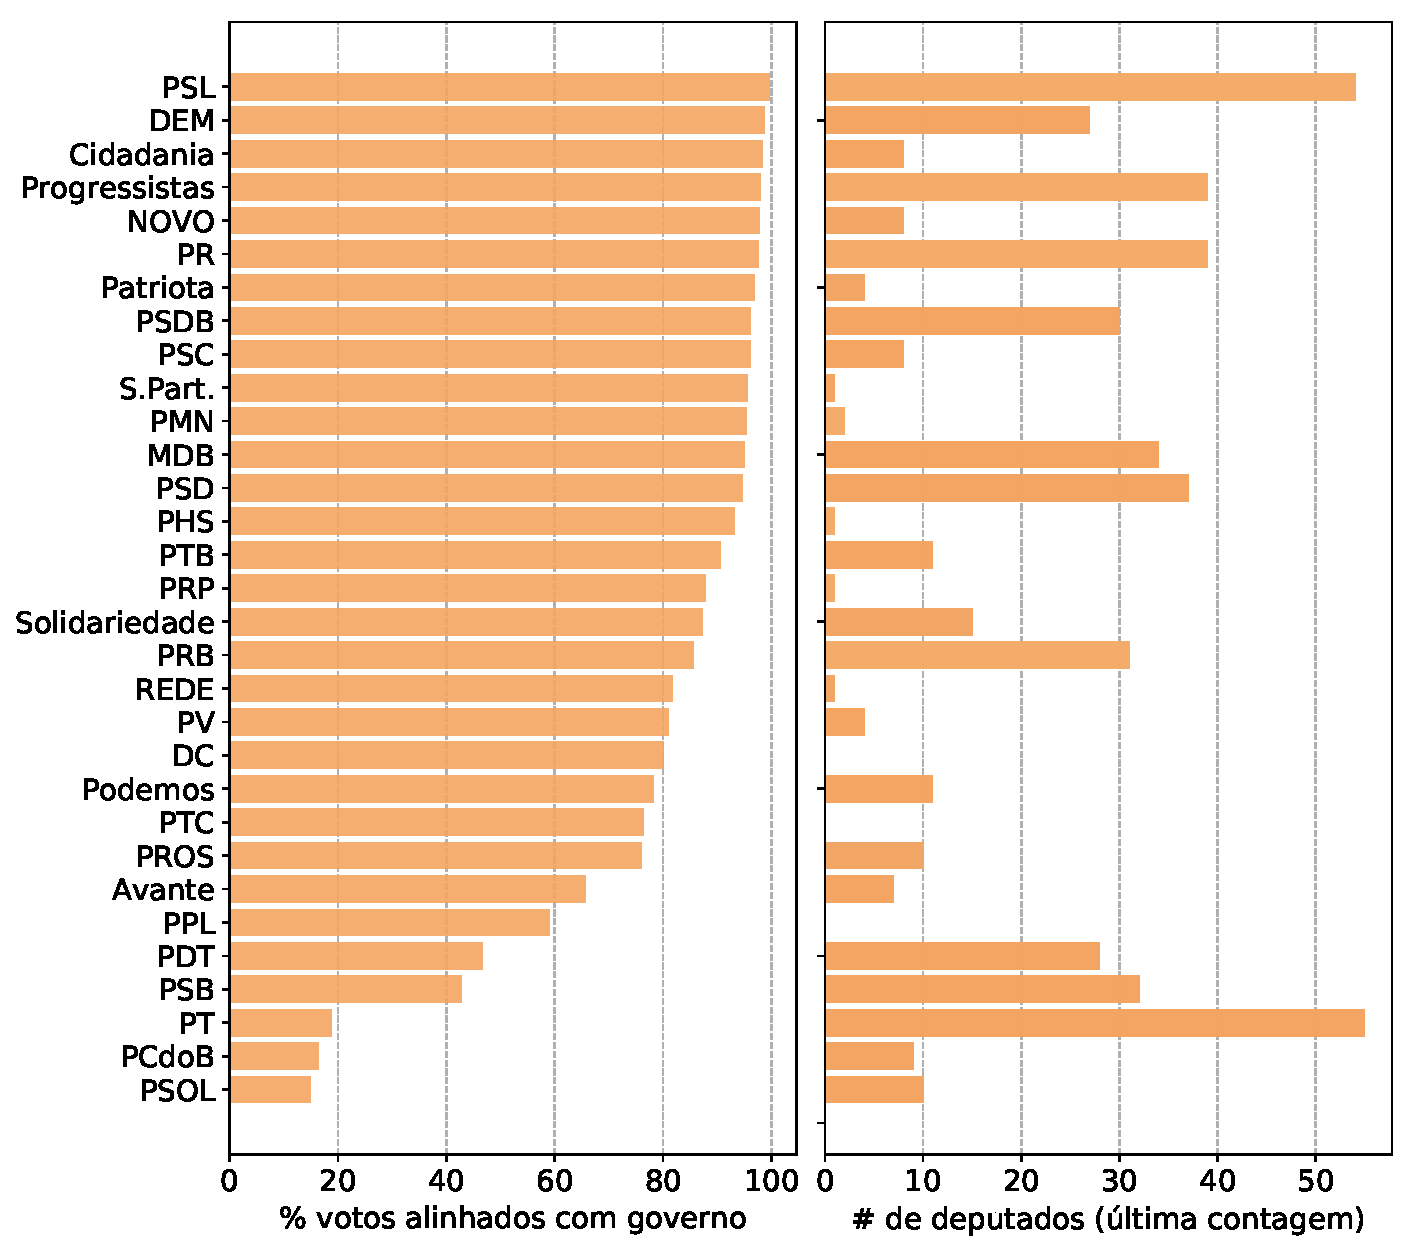
\includegraphics[width=1.0\textwidth]{graficos/apoio_ao_governo_partidos+tamanho_2019-05-09.pdf}
\caption{Fração de votos dos deputados que foram alinhados com a orientação do governo atual (painel esquerdo), e
  número de deputados de acordo com a última filiação, dentro de cada partido.}
\label{fig:apoio-governo-partido}
\end{figure} 

\begin{figure}[H]
\centering
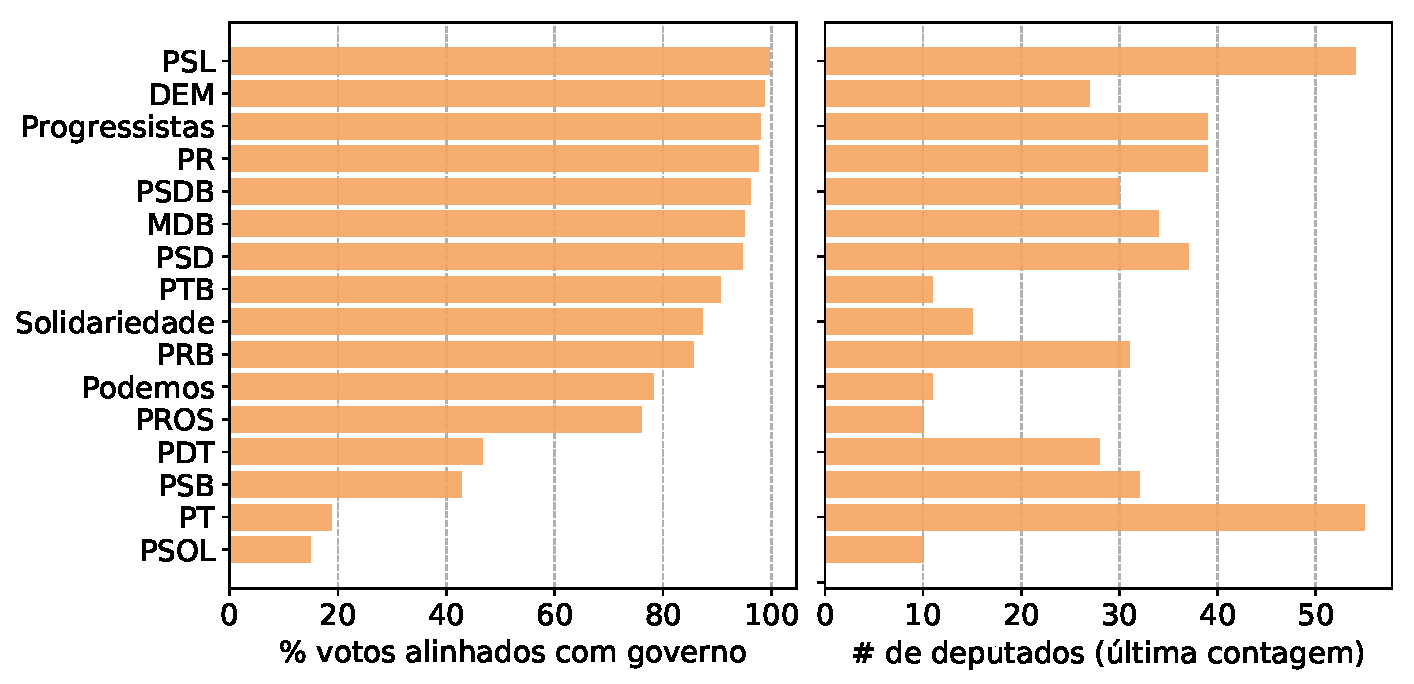
\includegraphics[width=1.0\textwidth]{graficos/apoio_ao_governo_partidos10+tamanho_2019-05-09.pdf}
\caption{Igual à Fig. \ref{fig:apoio-governo-partido}, mas para partidos com 10 deputados ou mais.}
\label{fig:apoio-governo-partido-G}
\end{figure} 

\subsubsection{Senado}

A análise do alinhamento dos votos dos senadores com o governo é dificultado pelo fato de que os dados abertos do senado não registram quem é ou foi o líder do governo no senado e nem qual foi a orientação dada. Para contornar esse problema, levantamos as datas de posse e saída de todos os líderes do governo no senado através de notícias, e utilizamos os votos deles como proxy da orientação do governo.

Em comparação com a câmara, vemos no senado, em todos os anos, um maior alinhamento com relação à orientação do governo, o que pode ser causado pelo fato do colegiado ser menor que a câmara, de forma que as matérias que chegam para votação já chegam com mais acordo.
Aqui também vemos um cenário de alinhamento com o atual governo, com grande parte dos senadores votando mais de 90\% das vezes junto com o líder (veja a Fig. \ref{fig:apoio-governo-senadores}). Também frisamos que só utilizamos votações não-secretas, que contabilizam cerca de 2/3 do total 
de votações no período, e que o número de votações disponíveis para análise é menor que na câmara: 12 contra 33. 

\begin{figure}[H]
\centering
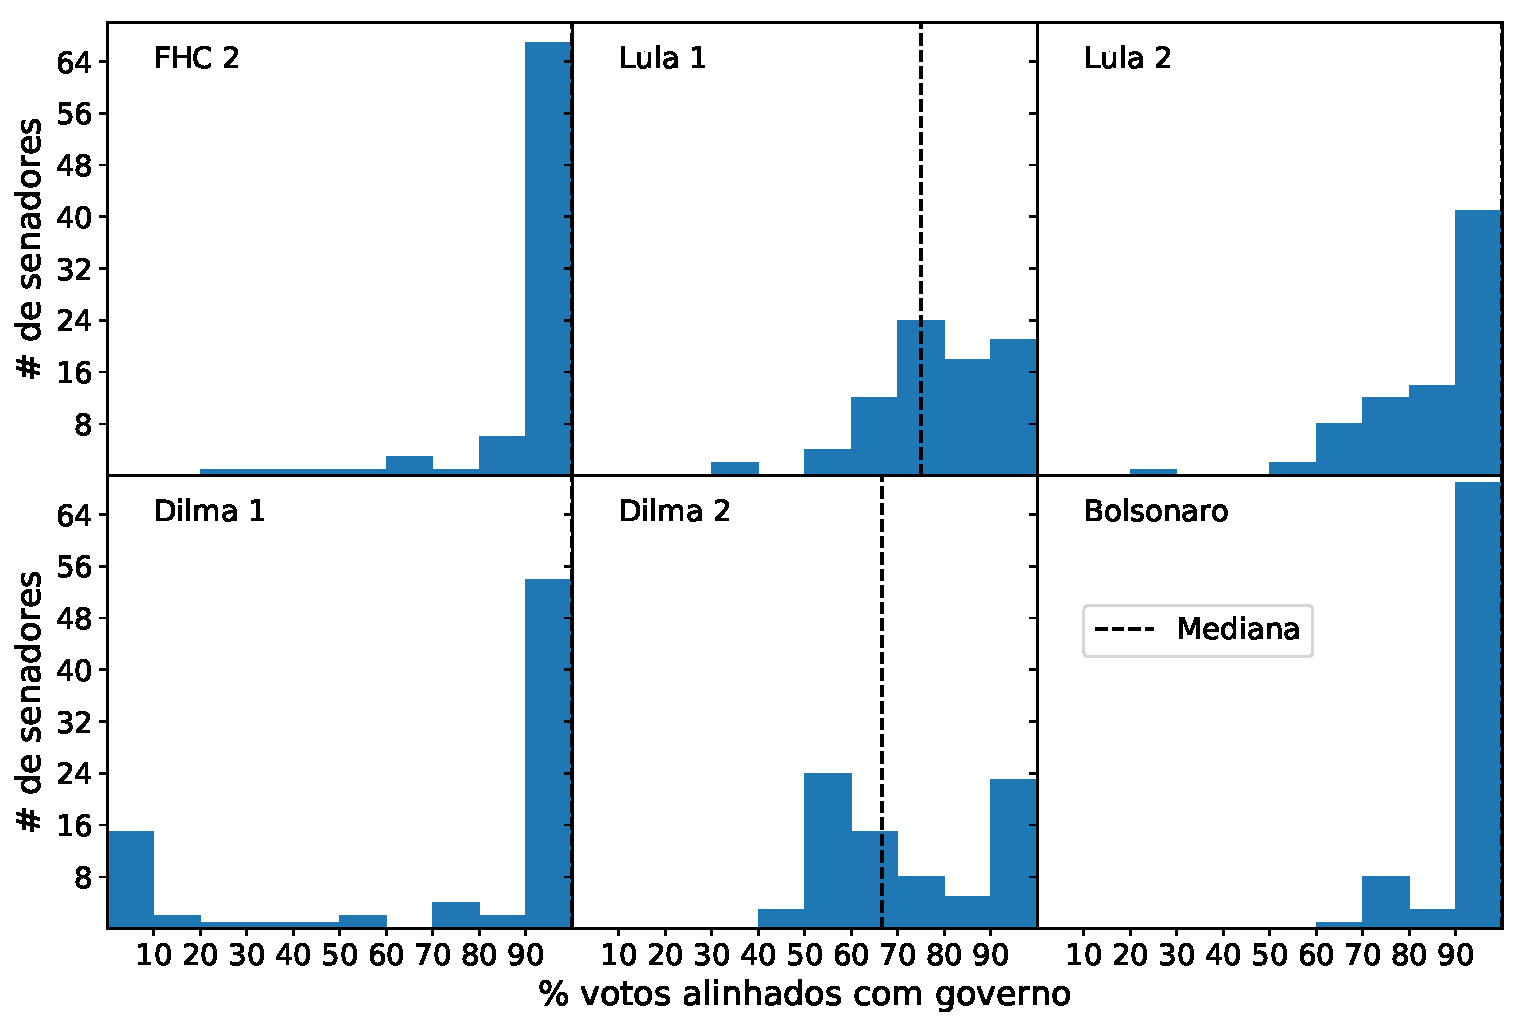
\includegraphics[width=1.0\textwidth]{graficos/senado/apoio_ao_governo_senadores_2019-05-09.pdf}
\caption{Contagem do número de senadores em função da fração de seus votos no plenário que se
  alinham com a orientação do governo. Cada painel apresenta os dados dos 100 primeiros dias de
  cada legislatura, discriminadas pelo presidente da república no período. A linha vertical tracejada preta
  separa a metade dos senadores com maior e menor alinhamento.}
\label{fig:apoio-governo-senadores}
\end{figure}

 A Fig. \ref{fig:apoio-governo-senadores} mostra que o atual senado votou tão alinhado com o governo quando o do segundo mandato de Fernando Henrique, talvez até um pouco mais. Assim como na câmara, é possível que nenhum assunto polêmico ou relevante tenha sido posto em pauta até o momento. Novamente, vemos os 100 dias do segundo mandato de Dilma com o menor alinhamento (podemos inclusive perceber indícios de polarização, dado que a distribuição apresenta dois picos).

Ao analisar o número de votos iguais aos do líder do governo, vemos no senado que o atual governo está bastante alinhado com os parlamentares nas 12 votações disponíveis (veja a Fig. \ref{fig:apoio-governo-votacao-senado}). De fato, o número médio de votos alinhados com o governo atual é o maior da série histórica. O segundo mandato de Dilma é, novamente, aquele que exibe o menor alinhamento médio dos 100 primeiros dias analisados. A variação entre as votações também é a maior de todas.

\begin{figure}[H]
\centering
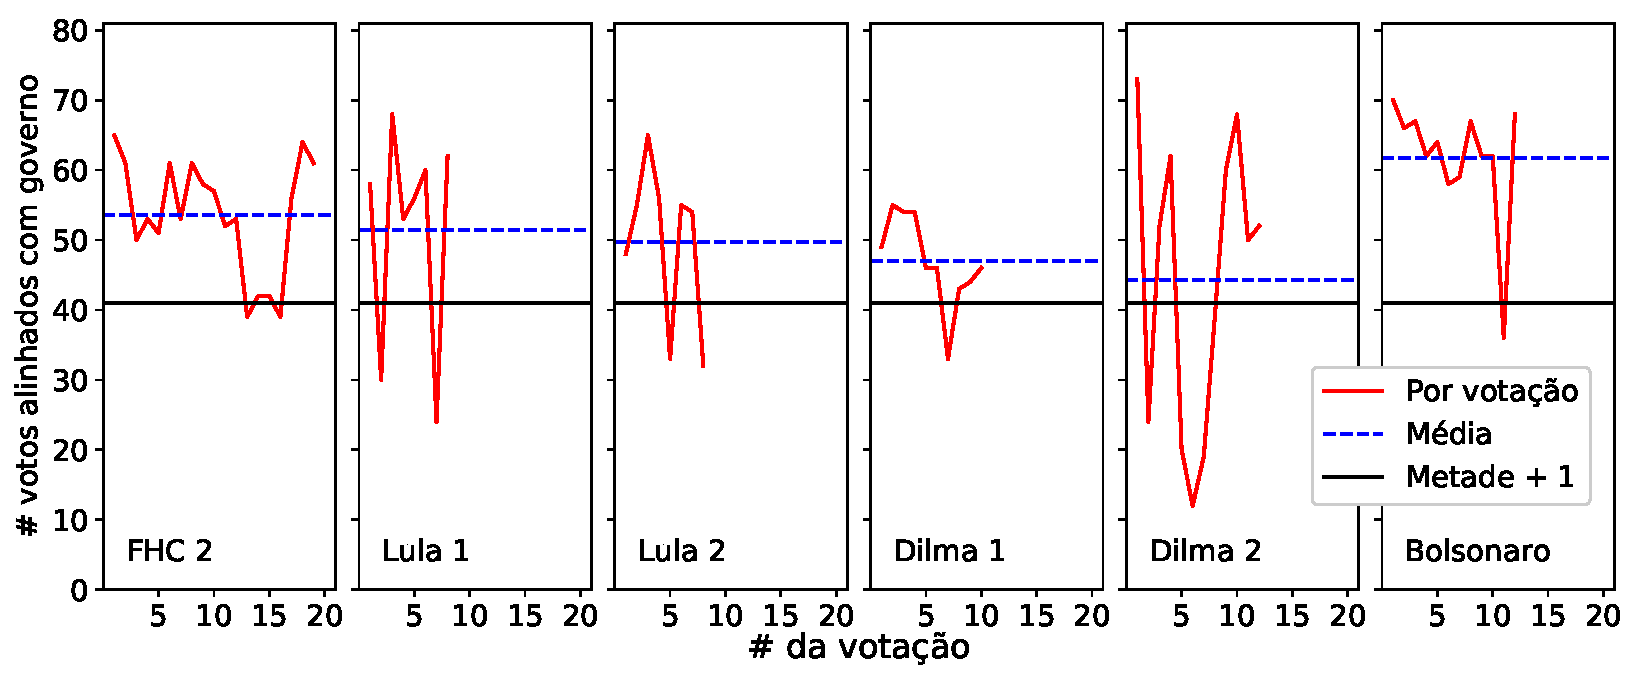
\includegraphics[width=0.9\textwidth]{graficos/senado/apoio_senado_ao_governo_por_votacao_2019-05-08.pdf}
\caption{Gráfico igual ao da Fig. \ref{fig:apoio-governo-votacao}, mas para o senado.}
\label{fig:apoio-governo-votacao-senado}
\end{figure} 

Finalmente, a Fig. \ref{fig:apoio-governo-partido-senado} mostra que o alinhamento dos partidos com o governo atual não é tão diversificado quanto na câmara. Todos os partidos apresentaram o mesmo voto que o líder do governo em ao menos 80\% 
das vezes. Aqui vale a ressalva de que, além de um número de votações menor, o número de parlamentares em cada partido também é menor do que na câmara, o que leva a maior flutuação estatística. 

A Tabela \ref{tab:apoio} apresenta as médias e medianas dos alinhamentos dos governos com os parlamentares ao longo das legislaturas, tanto para a câmara quanto para o senado.

\begin{table}[]
    \centering
    \caption{Para cada 100 primeiros dias de legislatura (identificadas pelo presidente em exercício), 
    apresentamos a média e mediana do alinhamento dos parlamentares com a orientação do governo, a média e mediana do número de votos alinhados com o governo (por votação), e o número de votações utilizadas na análise. A parte superior se refere à câmara, e a inferior, ao senado.}
    {\footnotesize
    \begin{tabular}{lccccc}
    \hline
 & \multicolumn{2}{c}{Alinhamento dep.} & \multicolumn{2}{c}{\# votos na câmara}   & \# votações \\
Governo & Média & Mediana & Média & Mediana & câmara \\
\hline
FHC 2 & 79\% & 100\% & 351 & 334 & 26 \\
Lula 1 & 76\% & 88\% & 306 & 302 & 21 \\
Lula 2 & 78\% & 96\% & 287 & 292 & 55 \\
Dilma 1 & 76\% & 92\% & 294 & 286 & 20 \\
Dilma 2 & 60\% & 64\% & 243 & 240 & 55 \\
Bolsonaro & 77\% & 95\% & 316 & 307 & 33 \\
\hline
& \multicolumn{2}{c}{Alinhamento sen.} & \multicolumn{2}{c}{\# votos no senado} & \# votações \\
Governo & Média  & Mediana & Média & Mediana & senado \\
\hline
FHC 2 & 94\% & 100\% & 53,6 & 53,0 & 19 \\
Lula 1 & 79\% & 75\% & 51,4 & 57,0 & 8 \\
Lula 2 & 87\% & 100\% & 49,8 & 54,5 & 8 \\
Dilma 1 & 74\% & 100\% & 47,0 & 46,0 & 10 \\
Dilma 2 & 73\% & 67\% & 44,3 & 51,0 & 12 \\
Bolsonaro & 95\% & 100\% & 61,8 & 63,0 & 12 \\
\hline
    \end{tabular}
    }
    \label{tab:apoio}
\end{table}


\begin{figure}[H]
\centering
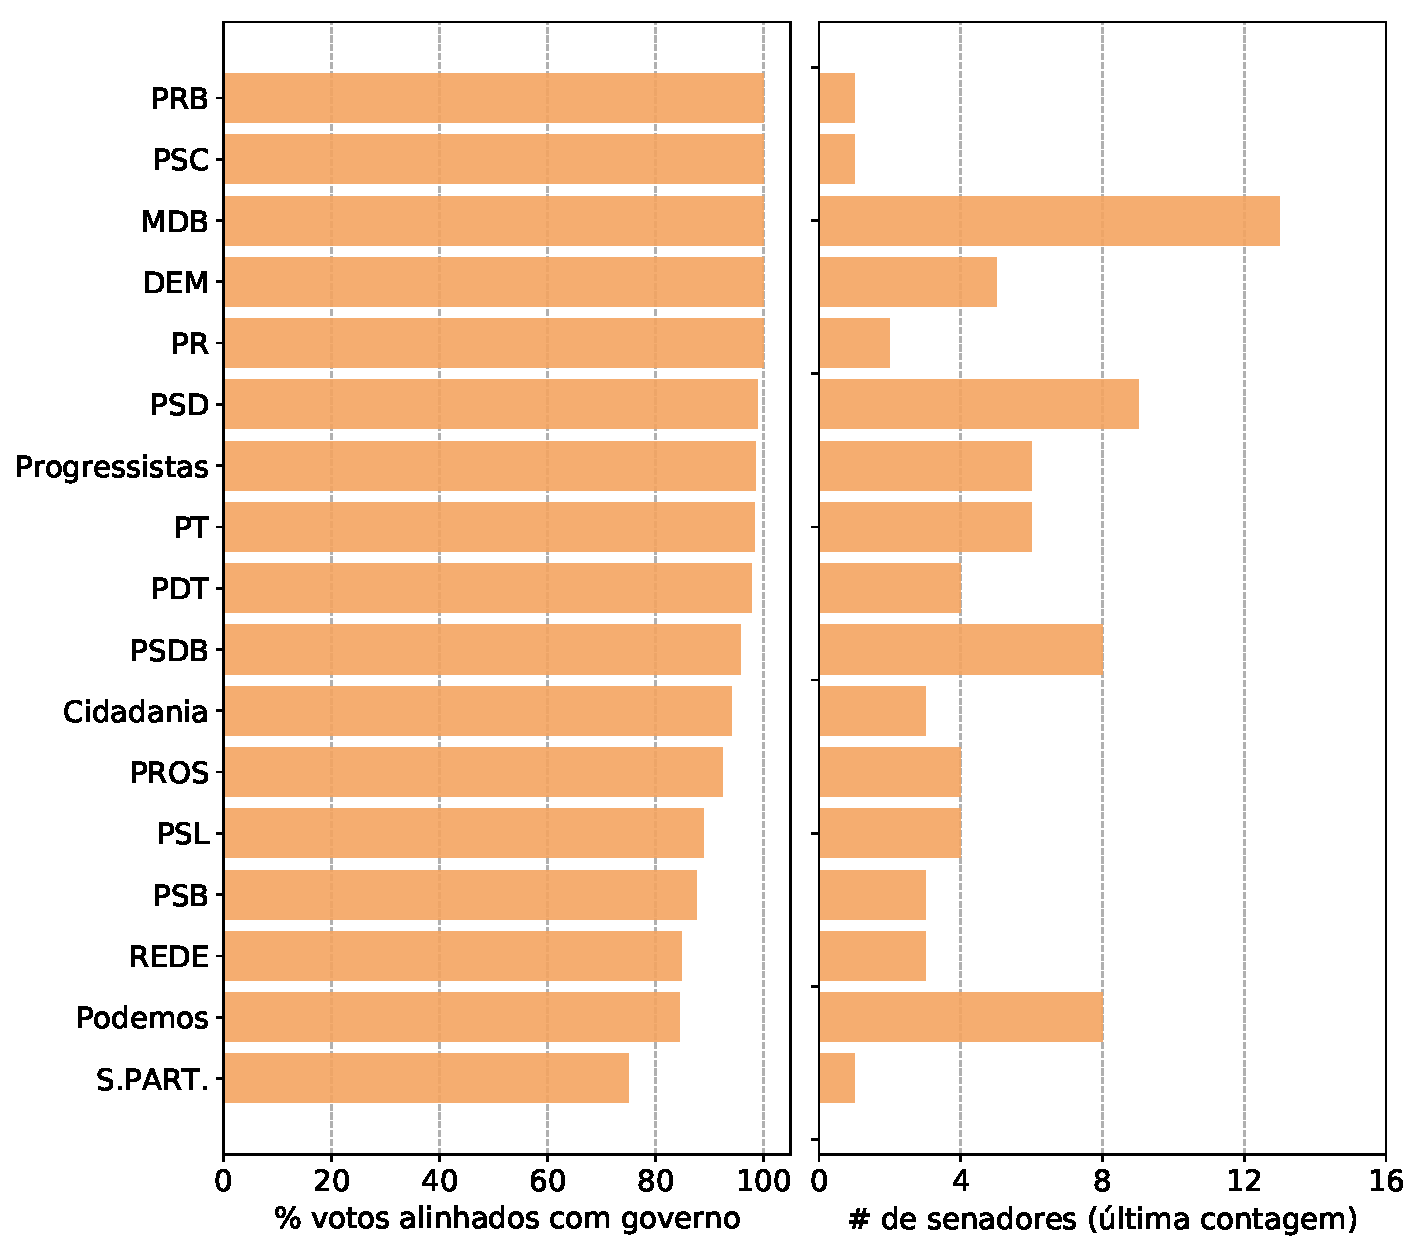
\includegraphics[width=1.0\textwidth]{graficos/senado/apoio_senado_ao_governo_partidos+tamanho_2019-05-09.pdf}
\caption{Fração de votos dos senadores que foram alinhados com a orientação do governo atual (painel esquerdo), e
  número de senadores de acordo com a última filiação, dentro de cada partido.}
\label{fig:apoio-governo-partido-senado}
\end{figure} 

\subsection{Fidelidade partidária}

Para estimar a fidelidade partidária, verificamos a fração de votos dos deputados que seguem
a orientação do próprio partido. Novamente, votações nas quais não houve orientação foram
ignoradas, assim como abstenções e ausências, e apenas foram consideradas votações nominais. É importante ressaltar que há muitos partidos com dados faltantes e/ou são compostos
por poucos parlamentares, o que resulta em amostras pequenas e com pouca representatividade estatística. 
A Tabela \ref{tab:alinha-dep} mostra o número de orientações recebidas por cada deputado.

O painel esquerdo da Fig. \ref{fig:fid-poder-partido} mostra que, tanto atual quanto historicamente, a maioria dos partidos
apresentam alta fidelidade, com mais de 80\% dos votos de seus deputados alinhados à sua orientação.
Para a maioria dos partidos, também observamos um ligeiro aumento do grau de fidelidade na legislatura atual.

\begin{figure}[H]
\centering
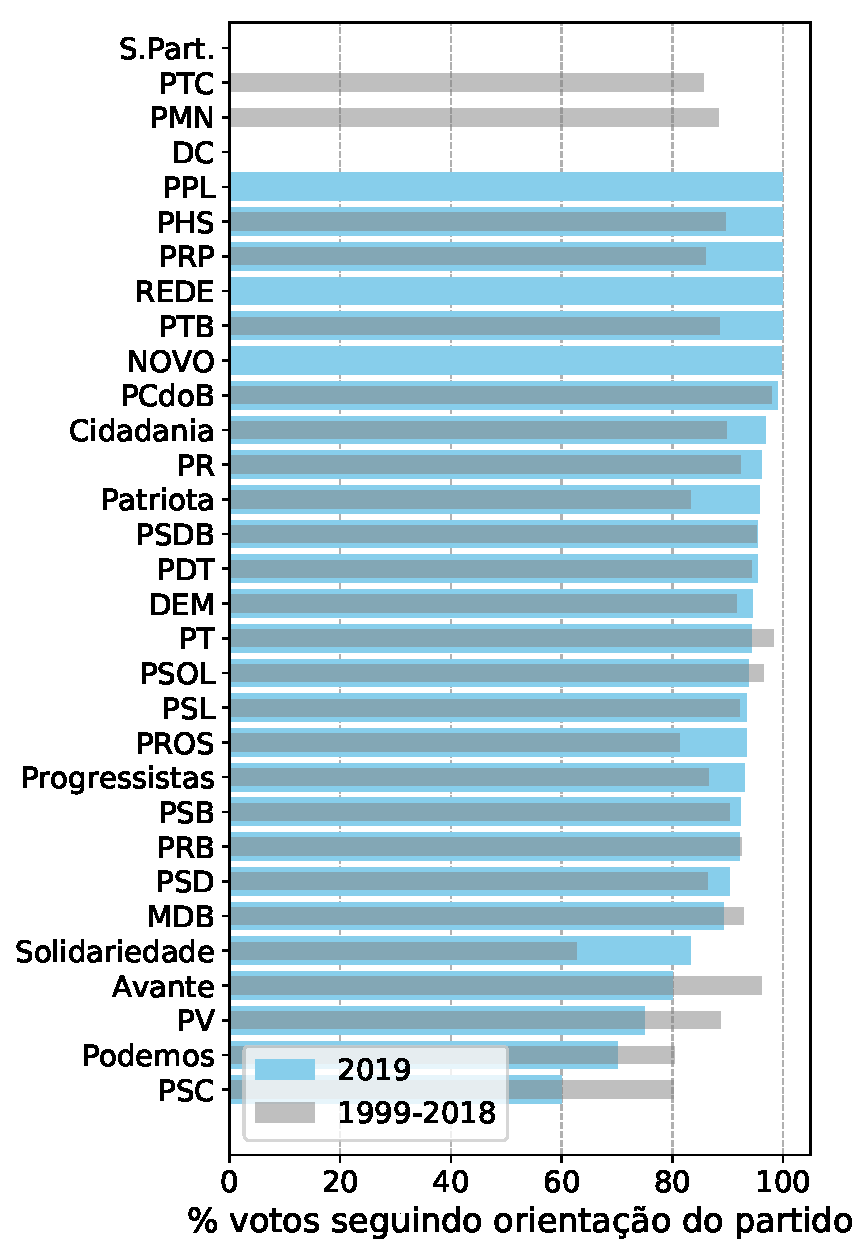
\includegraphics[width=0.49\textwidth]{graficos/fidelidade_partidaria_media_2019-05-08.pdf}
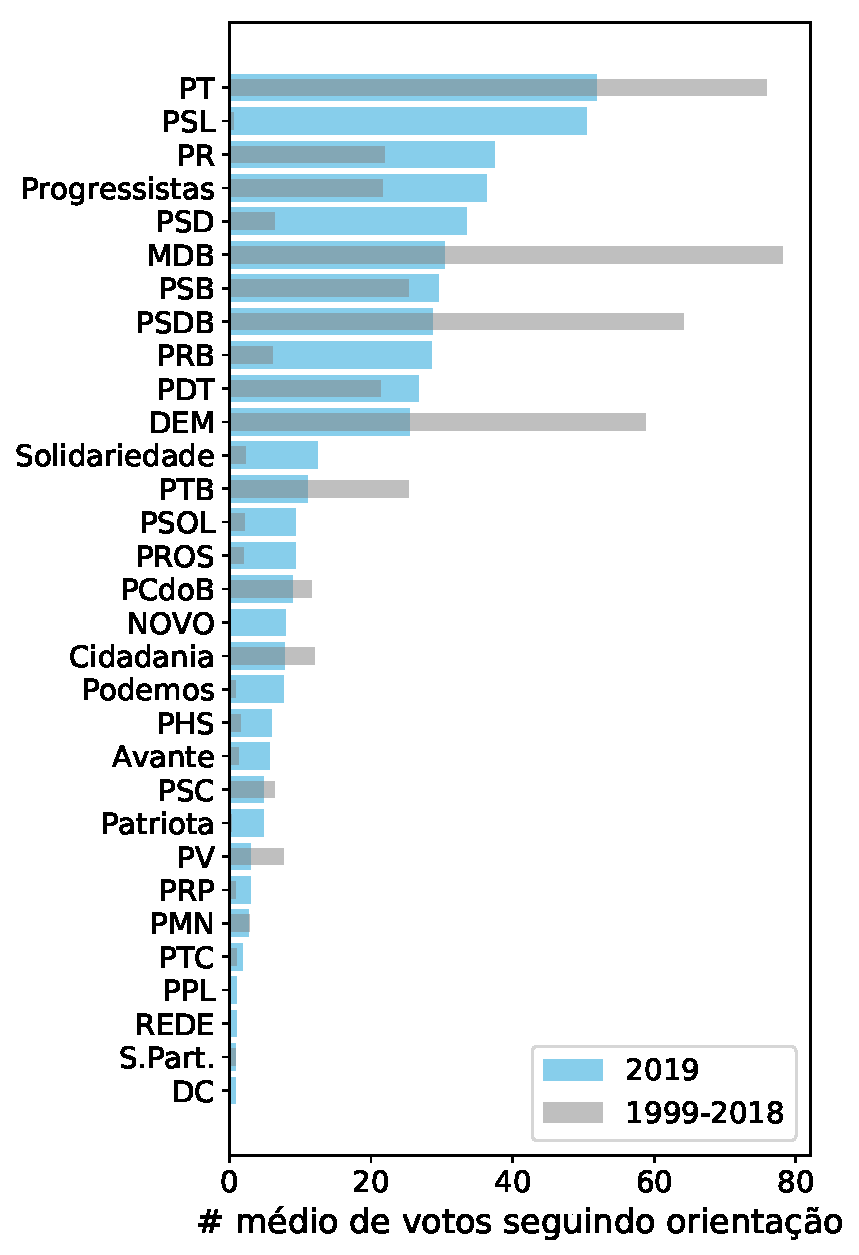
\includegraphics[width=0.49\textwidth]{graficos/poder_partidario_2019-05-08.pdf}
\caption{O painel esquerdo mostra a fração dos votos dos deputados que seguem orientação do próprio partido (que serve como indicador de fidelidade partidária). Já 
  o painel direito mostra o número médio de votos que seguem a orientação do próprio partido (que serve como uma estimativa de poder).
  As barras azuis e largas são para a atual legislatura, e as cinzas e estreitas são para o período
  histórico de 1999 a 2019.
}
\label{fig:fid-poder-partido}
\end{figure} 

O painel direito dessa mesma figura apresenta o grau de fidelidade multiplicado pelo tamanho da bancada
(ou tamanho médio, no caso do período histórico), o que dá o número de votos que o partido consegue
obter dada uma certa orientação. Essa capacidade de orientar um maior ou menor número de votos serve de proxy para o poder do partido. Uma vez que a fidelidade partidária não varia muito entre os partidos,
aqueles com as maiores bancadas (e.g. PT e PSL em 2019, MDB na série histórica) são também os com maior poder. Aqui destacamos que partidos outrora numerosos na câmara perderam
muitos assentos na legislatura atual (PT, PSDB, MDB e DEM), enquanto outros partidos, como o PSL e PRB,
tiveram crescimento significativo. De maneira geral, observamos na atualidade uma distribuição das
cadeiras entre um número maior de partidos.

\begin{figure}[H]
\centering
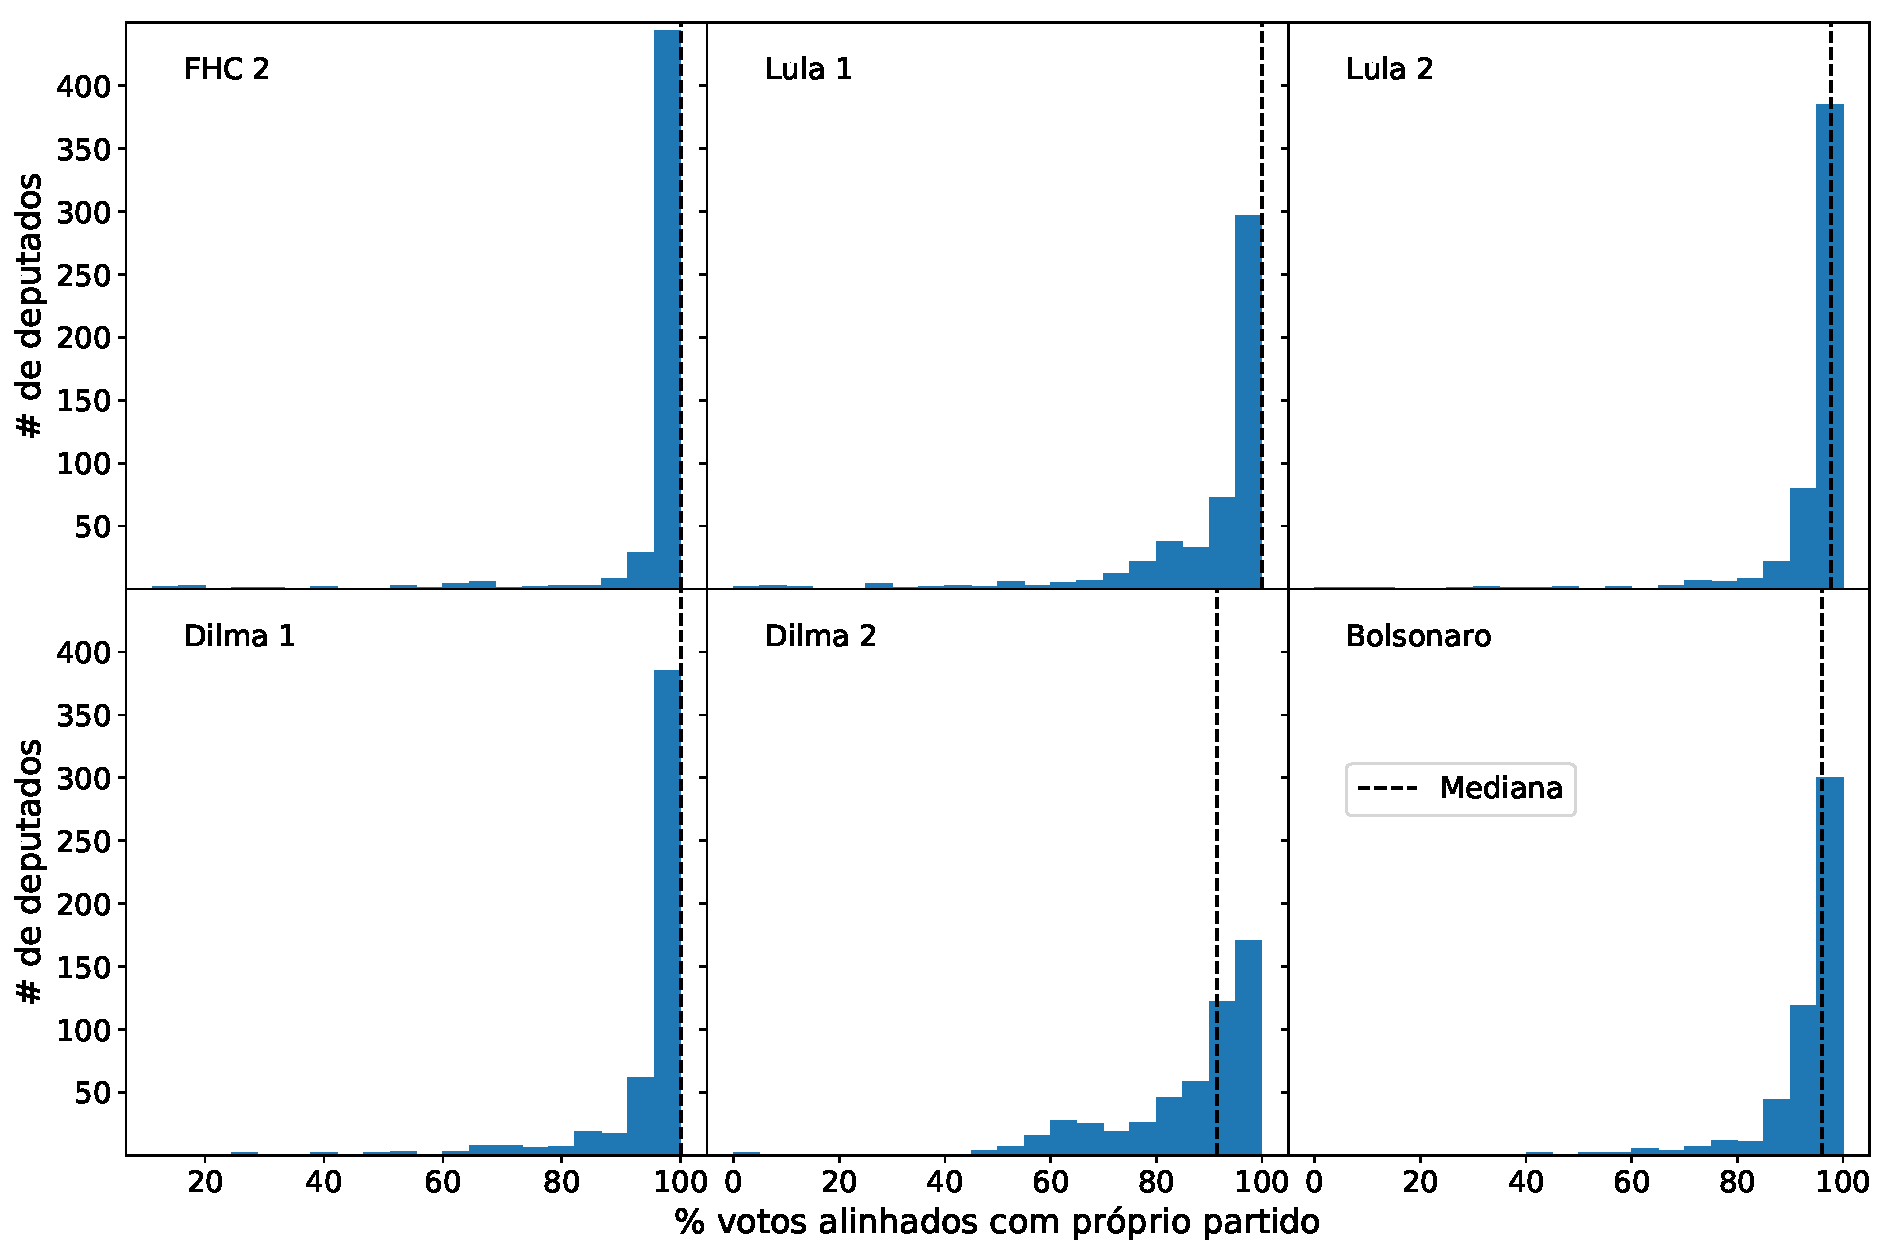
\includegraphics[width=1.0\textwidth]{graficos/fidelidade_partidaria_deputados_2019-05-09.pdf}
\caption{Histogramas da fração de votos dos deputados que são alinhados com o próprio partido, um para
  cada 100 primeiros dias de legislatura.}
\label{fig:fid-poder-deputado}
\end{figure} 

Por fim, a Fig. \ref{fig:fid-poder-deputado} mostra a distribuição dos deputados de várias legislaturas
em termos de fidelidade partidária. De maneira geral, ela é bastante concentrada em altos valores. Vemos
que a situação atual não difere muito do comportamento histórico e que, nos 100 primeiros dias da legislatura
anterior (segundo mandato de Dilma), a fidelidade partidária apresentou uma queda. 


%%%%%%%%%%%%%%%%%%%%%%%%%%%%%%%%%%%
\subsection{Atividade parlamentar}
\label{sec:atividade-parlamentar}

\subsubsection{Câmara}

Os deputados detém vários instrumentos para influenciar o processo legislativo. Nas várias etapas desse processo, cabem aos deputados e partidos se organizarem para influenciar a tramitação das proposições de interesse através de \textbf{ações legislativas}. Esse levantamento inicial de atividade parlamentar visa quantificar diferentes \textbf{ações legislativas} nos 100 primeiros dias da legislatura número 56.

Uma \textbf{ação legislativa} pode ser definida como a interação institucionalizada de um parlamentar em uma proposição. Por exemplo, o deputado Felipe Rigoni apresentou um Projeto de Lei. Ou mesmo, a deputada Tábata Amaral é relatora de uma Proposta de Emenda a Constituição. Dada essa estrutura e as restrições impostas pelos dados disponíveis, foi possível quantificar as ações apresentadas na Tabela \ref{tab:atividade-parlamentar-acao}.

\begin{table}
\caption{Tipos de ação parlamentar por quantidade de ações, quantidade de deputados, a mediana de ações dos deputados que tiveram alguma atividade, índice Gini e o acréscimo (ou decréscimo, se negativo) de alinhamento entre deputados que executam a ação e o governo, $A^*$, quando comparado com o alinhamento médio dos deputados. A quatidade de ação parlamentar por tipo pode ser maior que o número de objetos da ação porque um objeto pode ter mais de um deputado envolvido. Por exemplo, mais de um deputado pode propor um Projeto Legislativo.}
{\footnotesize
\begin{center}
\begin{tabular}{lrrrrr}
\toprule
{} &  \# Ações &  \# Deputados &  Mediana &  Gini & $A^*$\\
\midrule
apresentação PDL                  &      242 &          108 &      1.0 &  0.88 &  -38\% \\
apresentação PEC                  &       12 &           10 &      1.0 &  0.98 &  -3\% \\
apresentação PL                   &     2154 &          380 &      3.0 &  0.66 &  -1\% \\
apresentação REQ                  &     3569 &          480 &      5.0 &  0.50 &  -11\% \\
aprovações de requerimento        &       88 &           27 &      2.0 &  0.97 &   3\% \\
discussões de matéria             &      639 &          198 &      2.0 &  0.79 &  -11\% \\
obstruções em plenário            &       15 &            8 &      1.0 &  0.99 &  -21\% \\
pareceres de relatoria            &      184 &           93 &      1.0 &  0.88 &  -9\% \\
relatorias                        &     1879 &          398 &      3.0 &  0.59 &  -3\% \\
requerimento de audiência pública &      744 &          238 &      2.0 &  0.75 &  -18\% \\
requerimentos de informação       &      472 &          143 &      2.0 &  0.87 &  -27\% \\
\bottomrule
\end{tabular}
\end{center}
}
\label{tab:atividade-parlamentar-acao}
\end{table}

Como cada uma das \textbf{ações legislativas} tem uma função diferente dentro do processo legislativo, a comparação entre elas deve ser feita com cuidado. A primeira coluna da tabela \ref{tab:atividade-parlamentar-acao} é o número de vezes que a ação foi executada nos 100 primeiros dias da legislatura.\footnote{É importante observar que essa quantidade pode ser maior que a quantidade de objetos já que mais de um deputado pode ser o executor da ação.} \textit{Apresentação de Projeto de Lei, Apresentação de Requerimento e Relatorias} são as ações mais executadas e com mais deputados envolvidos. Naturalmente, são as ações com o menor Índice Gini, que mede se as ações estão concentradas em alguns parlamentares. Apesar do Gini das ações serem os mais baixos do grupo, um país considerado desigual tem Gini de 0.6. Portanto, pode-se afirmar que há poucos deputados responsáveis pela maioria das ações.

\begin{figure}[H]
\centering
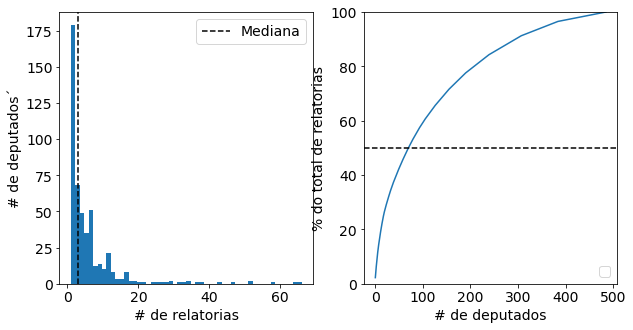
\includegraphics[width=1.0\textwidth]{graficos/camara/atividade/plot_relatorias_deputados.png}
\caption{O painel esquerdo mostra o histograma de número de relatorias. A linha vertical preta indica a mediana. O painel da direita apresenta o acumulado de relatorias por deputado. A linha horizontal preta representa o valor de 50\% das relatorias. }
\label{fig:atividade-parlamentar-relatorias-deputados}
\end{figure} 

As \textit{relatorias}, por exemplo, tem um Gini de 0.61. Em outras palavras, 40\% de todas as relatorias estão nas mãos de 50 deputados, que representam 9.7\% dos parlamentares (Figura \ref{fig:atividade-parlamentar-relatorias-deputados}). Apesar das relatorias serem distribuídas por membros das comissões que são escolhidos proporcionalmente ao tamanho das bancadas partidárias, existem parlamentares que são preferenciais para obter relatorias. Uma hipótese para explicar esse fenômeno é o custo não desprezível de trabalho e baixo apelo popular. A relatoria, diferente de presença no plenário, não é uma ação acompanhada pelo eleitorado. Também, há um custo político de negociar a relatoria além do custo laboral de elaborar um parecer. Portanto, o deputado médio teria pouco incentivo e custo alto para relatar uma matéria. 

Porém, apesar de haver muitas relatorias, poucas já tiveram seus pareceres entregues, somente 184, apenas 9.7\% do total. Esse é um fenômeno que pode explicar a razão para a qual somente poucas proposições estão prontas para a pauta do plenário. Parlamentares, seja por motivos políticos de bloqueio da proposição, seja por inépcia, não entregam os pareceres no prazo estipulado pelo regimento interno da Câmara. Isso afeta o andamento da proposição e, por consequência, a quantidade de proposições prontas para a pauta.

\begin{figure}[H]
\centering
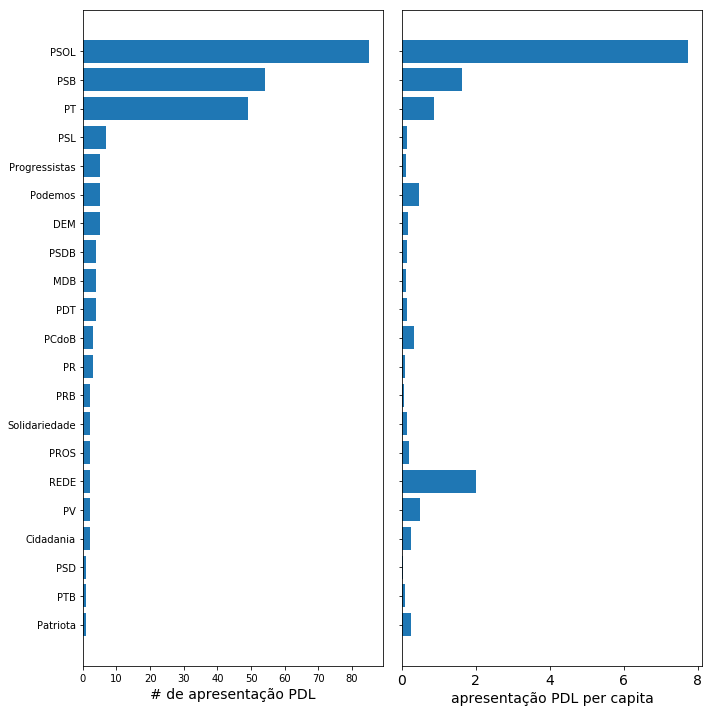
\includegraphics[width=1.0\textwidth]{graficos/camara/atividade/PDL.png}
\caption{O painel esquerdo mostra o número de Propostas de Decreto Legislativo (PDL) que cada partido apresentou nos primeiros 100 dias. O esquerdo mostra o número de PDLs por deputado no partido. }
\label{fig:atividade-parlamentar-pdl-partidos}
\end{figure} 

As \textbf{ações legislativas} também podem ser usadas para descrever estratégias que os partidos adotam na prática legislativa. A Figura \ref{fig:atividade-parlamentar-pdl-partidos} mostra que PSOL, PSB e PT têm 85, 54 e 49 apresentações de Projeto de Decreto Legislativo (PDL), que juntos correspondem a 77\% do total. Segundo o Glossário de Termos Legislativos, o PDL visa "regular as matérias de competência exclusiva do Poder Legislativo, sem a sanção do Presidente da República". Esse tipo legislativo é comumente usado para sustar atos do executivo e, como vimos na Figura \ref{fig:atividade-parlamentar-pdl-partidos}, é usado por alguns partidos pouco alinhados com o governo, como mostra a Figura \ref{fig:apoio-governo-partido}. Porém, curiosamente, o PCdoB que é o partido mais desalinhado com o governo, não apresentou PDLs. 

\begin{figure}[H]
\centering
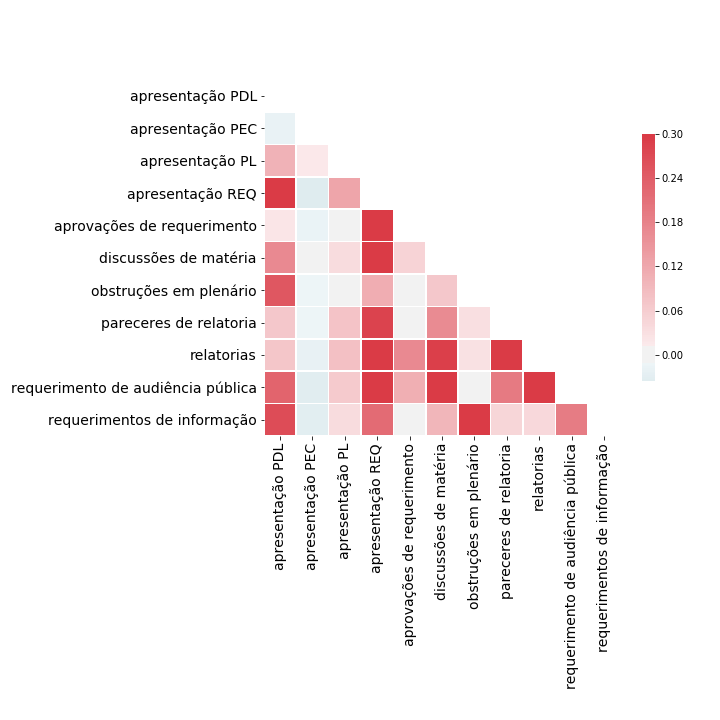
\includegraphics[width=1.0\textwidth]{graficos/camara/atividade/plot_corr_relatorias_deputados.png}
\caption{Correlação Pearson das ações parlamentares dos deputados. A escala de correlação varia de -1 a 1. Portanto, o azul claro representa baixa correlação e o vermelho correlação positiva média.}
\label{fig:atividade-parlamentar-corr}
\end{figure} 

As estratégias legislativas também podem ser executadas por grupos de parlamentares. A figura \ref{fig:atividade-parlamentar-corr} é uma matriz de correlação de Spearman das atividades dos deputados. Notamos que algumas \textbf{ações legislativas} são mais correlacionadas a outras. Por exemplo, parlamentares que pedem \textit{requerimentos de informação} tendem a fazer \textit{obstruções em plenário} e \textit{apresentar PDLs}, que vamos chamar de comportamento A. Todas essas ações têm consequência direta tanto no andamento das proposições da situação quanto no escrutínio dos atos do governo. Por outro lado, há outro grupo que apresenta \textit{requerimentos de audiência pública}, \textit{discute matérias} e tem \textit{relatorias}, que chamaremos de comportamento B. Esse grupo tem mais poder sobre a pauta da discussão legislativa e andamento das proposições. Tanto as audiências públicas quanto as relatorias são instrumentos para acelerar ou frear o andamento de certas proposições e temas. Além do controle sobre o andamento, a ação de \textit{discussões de matérias} mostra que o grupo tem espaço de fala nas comissões e plenário.

Também podemos entender as \textbf{ações parlamentares} a partir do alinhamento dos deputados que as executaram. Dessa forma, queremos saber se as ações são mais praticadas por deputados alinhados ou não ao governo. Para isso, considere que um grupo de \textbf{ações parlamentares}, $a$, pode ser executada diversas vezes por um deputado $d$. Assim, o número de \textbf{ações parlamentares} executadas por um deputado é $a_d$.  Cada deputado também tem uma taxa de alinhamento com o governo, $g_d \in [0, 1]$. Queremos saber se uma \textbf{ação parlamentar} foi mais executada por quem tem alinhamento ou não. Uma boa maneira de medir isso é simplesmente multiplicando as duas quantidades para cada parlamentar e somando para todos os parlamentares,

\[A(a, g) := \sum_{d=1}^D g_d a_d, \]
onde $D$ é o número de parlamentares ativos no intervalo de tempo e $A(a,g)$ é o alinhamento das ações com o governo. 

Dessa maneira, se todos os parlamentares estiverem completamente alinhados com o governo, ou seja $g_d = 1$, então $A(a,g) = \sum_{d} a_d$ que é simplesmente o número de ações. Caso contrário, de completo desalinhamento,$g_d = 0$, então  $A(a,g) =0$.  Vemos que $A(a,g) \in [0, \sum_{d\in D} a_d]$, mas para conseguirmos comparar diferentes ações em diferentes intervalos de tempo, vamos normalizar $A(a,g)$. Portanto,

\[A(a, g) := \frac{\sum_{d=1}^D g_d a_d}{\sum_{d=1}^D a_d}, \]
onde $A(a,g) \in [0,1]$. Usando o alinhamento do deputado $d$ como referência de alinhamento para a ação que ele executa, podemos interpretar  $A(a,g)$ como o alinhamento médio do grupo de ações $a$ em relação ao governo.

\begin{comment}
Finalmente, se 
\begin{equation}
\frac{a_d}{\sum_{d=1}^D a_d} = g_d,
\end{equation}
então temos uma situação em que as ações estão distribuídas de acordo com o alinhamento com o governo, i.e., deputados mais alinhados executaram mais ações e deputados menos alinhados executaram menos ações. Essa pode ser considerada uma situação onde há um equilíbrio do uso das ações. Situação tal que pode ser usada como base para entender se uma ação é mais usada por algum espectro do alinhamento. Assim, definimos $A^*(a,g)$ por $A(a,g) - A(g, g)$

\[A^*(a,g) := \frac{1}{\sum_{d\in D} a_d}(\sum_{d\in D} g_d^2 - \sum_{d\in D} g_da_d) \in [-1,1]\]
\end{comment}

Se um certo grupo de ações $a$ se distribuir igualmente entre todos os parlamentares, 
independentemente da orientação desses em relação ao governo, ela seria considerada neutra; além disso, ela teria um alinhamento médio igual ao alinhamento médio dos deputados. Por outro lado, se essas ações se concentrassem em parlamentares menos alinhados, elas seriam interpretadas como instrumentos de oposição; além disso, elas teriam alinhamento médio abaixo da média dos deputados. Assim, definimos 
$A^*(a,g) := A(a,g) - A(1,g)$ como o indicador de quem mais utiliza a ação $a$, 
onde $A(1,g)$ é o alinhamento médio dos deputados ao governo: $A^*(a,g)<0$ indica que 
$a$ é utilizada preferencialmente por deputados com alinhamento menor que a média, e $A^*(a,g)>0$ indica que $a$ é utilizada por quem é mais alinhado ao governo.

A figura \ref{fig:atividade-parlamentar-acao-apoio} mostra que as ações \textit{apresentação de PL, relatorias e apresentação de PEC} estão muito próximas de $A(1,g)$. Ou seja, são ações que se distribuem igualmente independente da alinhamento com o governo. A única ação que é executada majoritariamente por membros do governo é a \textit{aprovação de requerimento}. Por outro lado, ações como \textit{apresentação de PDL, requerimento de informação, obstrução em plenário e requerimento de audiência pública} são usadas por deputados com pouco alinhamento com o governo.

Podemos dizer, então, que parlamentares com comportamento A são menos alinhados com o governo, o que era esperado já que essas ações tendem a deixar o andamento legislativo mais lento e questionar as ações do executivo. Os parlamentares com comportamento B estão mais alinhados com o governo que os do A. Porém, tampouco são alinhados ao governo, já que suas ações apresentam $A^* > 0.1$.

\begin{figure}[H]
\centering
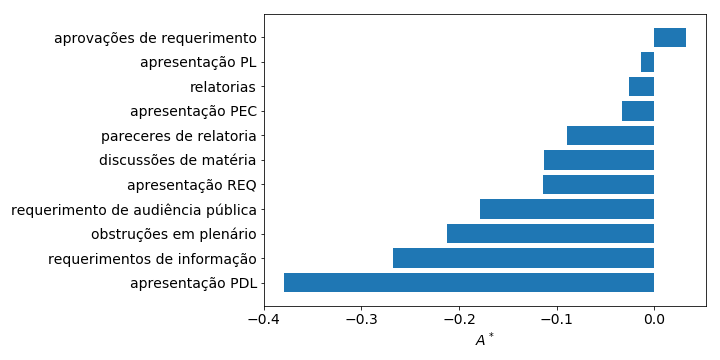
\includegraphics[width=1.0\textwidth]{graficos/camara/atividade/a_estrela.png}
\caption{Alinhamento dos parlamentares que executaram a ação, $A^*$, na Câmara. A ação \textit{deputado\_numb} representa $A(g,g)$ que deve ter o valor 0.}
\label{fig:atividade-parlamentar-acao-apoio}
\end{figure} 

Esta breve exposição da atividade parlamentar na Câmara mostrou que é possível quantificar e discernir o trabalho feito pelos deputados com mais precisão. Com isso os parlamentares podem ser descritos e ordenados para além da apresentação de PL e votação.\footnote{As figuras das outras \textbf{ações parlamentares} estão em anexo.} Também é possível fazer o mesmo para partidos e entender seu comportamento e estratégia. Porém, ainda há muitos pontos de expansão e exploração da atividade parlamentar. Além de comparações históricas sobre o comportamento dos parlamentares, é possível construir modelos mais robustos para a identificação de padrão de comportamentos.

\subsubsection{Senado}

\begin{figure}[H]
\centering
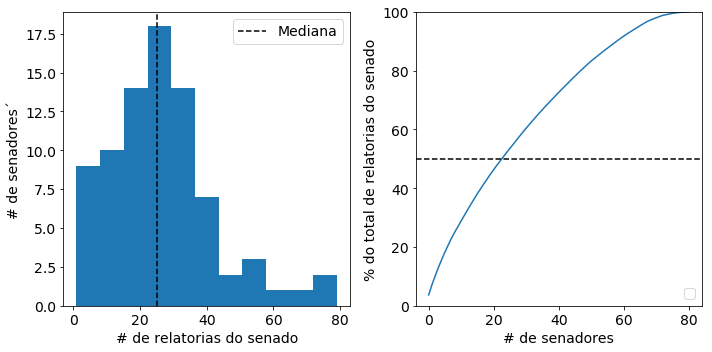
\includegraphics[width=1.0\textwidth]{graficos/camara/atividade/plot_relatorias_senado_senadores.png}
\caption{O painel esquerdo mostra o histograma de número de relatorias no Senado. A linha vertical preta indica a mediana. O painel da direita apresenta o acumulado de relatorias por senador. A linha horizontal preta representa o valor de 50\% das relatorias. }
\label{fig:atividade-parlamentar-relatoria-senadores}
\end{figure} 

Da atividade parlamentar do senado, capturamos as relatorias por senador, cuja distribuição é apresentada na Figura \ref{fig:atividade-parlamentar-relatoria-senadores}. Nela observamos também uma concentração de relatorias, porém em menor proporção que na Câmara. 40\% das relatorias estão com 20 senadores, que correspondem a 24.7\% dos senadores. Na Câmara, por outro lado, 40\% das relatorias estão com somente 9.7\% dos senadores. Nos termos do índice Gini que mede a desigualdade na distribuição, vemos que enquanto o da Câmara é 0.61 o do Senado é de 0.36. Uma hipótese para explicar tal diferença é que o Senado é uma casa legislativa menor, com somente 81 parlamentares contra 513 da Câmara, mas sua estrutura não é proporcionalmente menor. O número de comissões e posições na mesa é tal que os senadores tem mais cargos per capita que na Câmara. Dessa maneira, os senadores tem mais influência e poder legislativo proporcional que os deputados. Como a relatoria é uma maneira de exercer influência no processo legislativo, a distribuição é mais equânime.


%%%%%%%%%%%%%%%%%%%%%%%%%%%%%%%%%%%%%%%%%%
\subsection{Distribuição de cargos e poder}
\label{sec:cargos-deputados}

A proposta desta seção é verificar como os cargos em comissões e lideranças de blocos e partidos,
de maneira conjunta, são distribuídos entre os deputados. Aqui, infelizmente, temos dificuldades com a base de dados
abertos da câmara: parlamentares cuja participação em comissões é conhecida ou listada no portal
da câmara não aparecem como participantes dos órgãos. Os casos da deputada Tabata
Amaral\footnote{\footurl{http://www.camara.leg.br/deputados/204534}\\
  \footurl{https://dadosabertos.camara.leg.br/api/v2/deputados/204534/orgaos?ordem=ASC\&ordenarPor=dataInicio}}
(membro titular na Comissão de Educação) e do deputado
Ted Conti\footnote{\footurl{http://www.camara.leg.br/deputados/206231}\\
  \footurl{https://dadosabertos.camara.leg.br/api/v2/deputados/206231/orgaos?ordem=ASC\&ordenarPor=dataInicio}}
(membro titular na Comissão de Ciência e Tecnologia, Comunicação e Informática) são exemplos desse
problema. A Fig. \ref{fig:orgaos-por-ano} mostra que o ano de 2019 apresenta um registro atípico de número
de vagas preenchidas para um início de legislatura, evidenciando o problema. Além disso, e figura mostra que dados anteriores a 1999 estão
ausentes.

\begin{figure}[H]
\centering
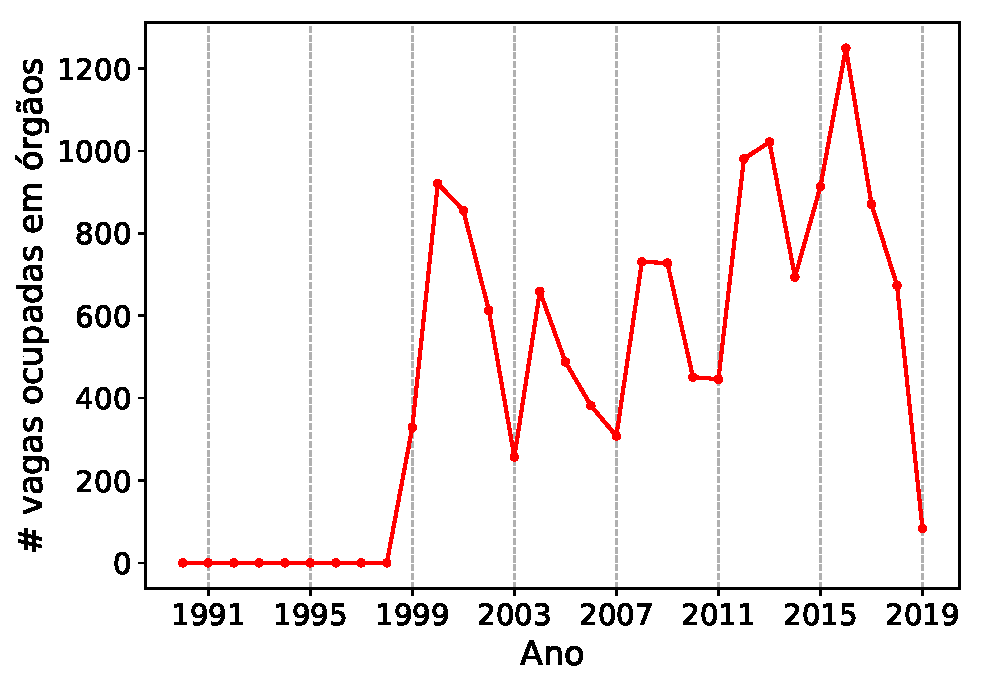
\includegraphics[width=0.7\textwidth]{graficos/orgaos-ocupados-por-ano_2019-05-02.pdf}
\caption{Número de vagas preenchidas por deputados no período de 1 de fevereiro a 18 de abril em órgãos (incluindo Mesa Diretora,
  Grupos de Trabalho, Comissões Parlamentares de Inquérito, Comissões Permanentes, Especiais, Mistas e Externas,
  Conselhos e Subcomissões, entre outros) ao longo dos anos, de acordo com a base de dados abertos da câmara dos deputados.}
\label{fig:orgaos-por-ano}
\end{figure} 

Pelo motivo apresentado acima, apenas uma análise histórica da participação em comissões pode ser feita. Por outro lado,
a base de dados abertos não guarda as informações sobre lideranças passadas dos blocos e partidos, de maneira
que não é possível realizar uma análise histórica conjunta entre participação em comissões e lideranças.

Um aspecto interessante da Fig. \ref{fig:orgaos-por-ano} é a marcada sazonalidade na ocupação de cargos.
O número de cargos preenchidos são máximos nos segundos e terceiros anos de cada legislatura. Essa sazonalidade
também é observada se nos concentrarmos apenas em participação em comissões e na mesa diretora da câmara
(cargos mais importantes politicamente), conforme mostra a Fig. \ref{fig:cargos-por-ano}.

\begin{figure}[H]
\centering
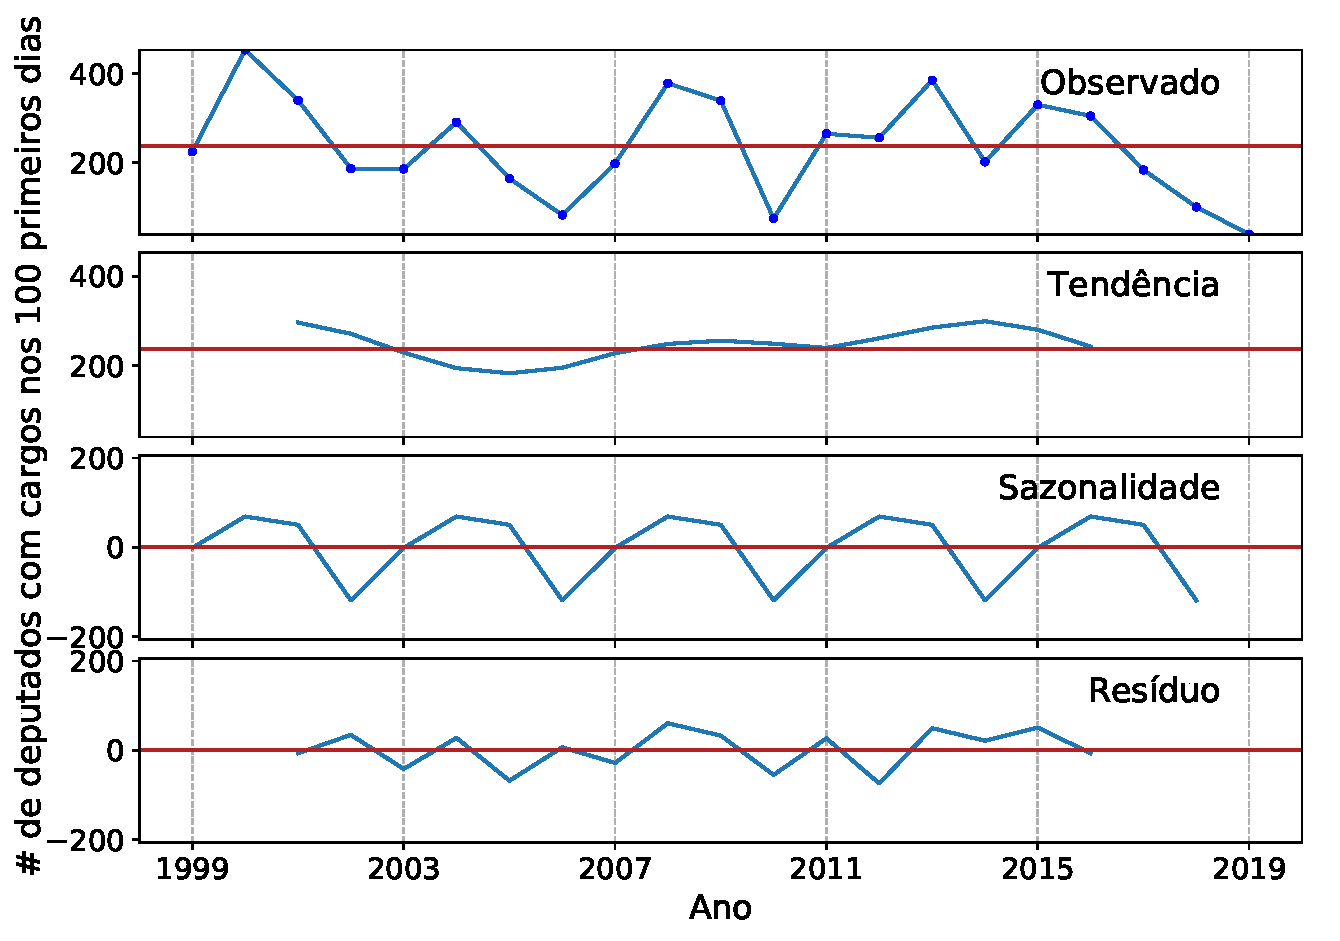
\includegraphics[width=0.9\textwidth]{graficos/cargos_sazonalidade_2019-05-06.pdf}
\caption{Número de vagas preenchidas por deputados no período de 1 de fevereiro a 18
  de abril em comissões e mesa diretora (painel superior). Os painéis seguintes mostram os termos aditivos
  de sua decomposição em tendência, sazonalidade e resíduo.}
\label{fig:cargos-por-ano}
\end{figure} 

Também focando nas comissões e mesa diretora, analisamos por quanto tempo as vagas ficam preenchidas por um mesmo
deputado (veja a Fíg. \ref{fig:tempo-na-vaga}). Existe uma regularidade clara entre as legislaturas, onde a ampla
maioria dos cargos são preenchidos por até um ano, sendo que um ano é o tempo de permanência mais frequente
(i.e. moda). Também é possível observar um pequeno segundo pico de tempo de permanência em até 36 dias na maioria
das legislaturas. Embora não seja possível observar no gráfico, as legislaturas em geral apresentam alguns poucos
casos nos quais um cargo é ocupado por mais de três anos (chegando a quatro). Esses são cargos de membro da mesa
diretora e relator de comissão especial. Por fim, a $53^{\mathrm{\underline{a}}}$ legislatura apresenta um pico em cerca
de 100 dias após o primeiro ano, possivelmente relacionado a algum acontecimento específico.

\begin{figure}[H]
\centering
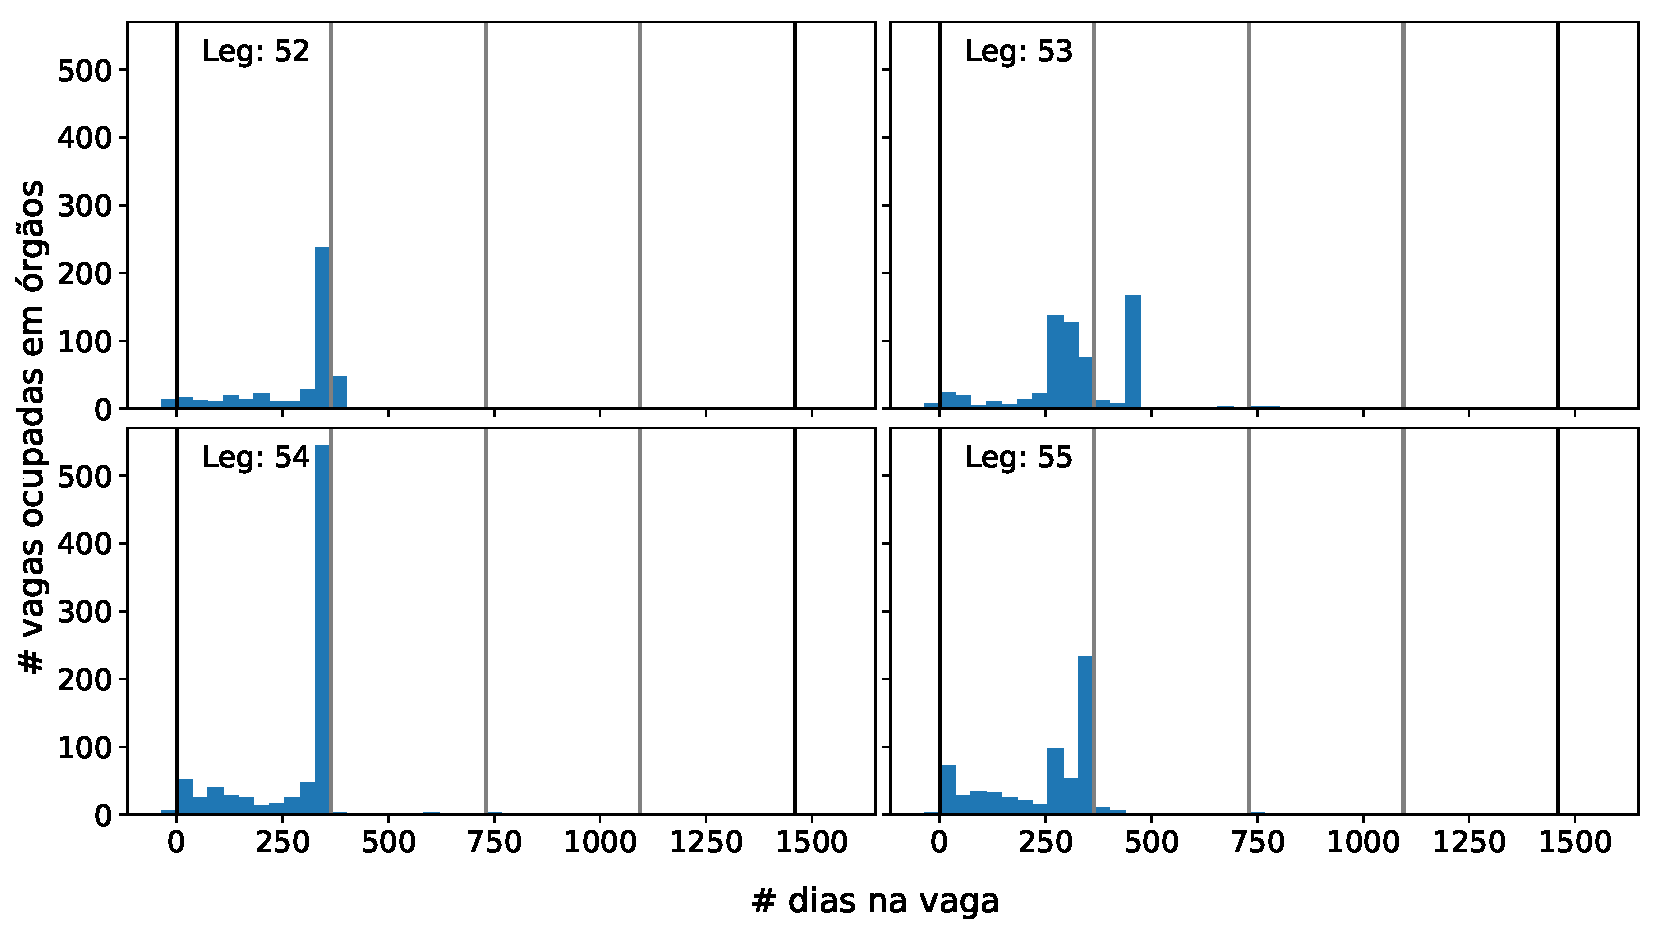
\includegraphics[width=1.0\textwidth]{graficos/vagas_ocupadas_por_tempo_na_vaga_2019-05-06.pdf}
\caption{Número de vagas ocupadas em comissões e mesa diretora em função do número de dias em que o deputado
  ocupou a vaga. Cada painel retrata uma legislatura anterior a atual, desde a $52^{\mathrm{\underline{a}}}$,
  que começou em 2003. As linhas verticais marcam o número de anos de permanência na vaga, sendo que as linhas
  verticais pretas marcam durações de zero anos (e zero dias) e de 4 anos. As colunas têm largura de 36,5 dias,
  excluem valores na borda inferior e incluem valores na borda superior.)
}
\label{fig:tempo-na-vaga}
\end{figure} 

%\HX{Incluir análise histórica da distribuição de cargos}

%%%%%%%%%%%%%%%%%%%%%%%%%%%%%%%%%%%
\subsection{Uso da cota parlamentar}
\label{sec:cota-parlamentar}

Conforme apresentado na Seção \ref{sec:intro}, as bases de dados relacionadas às despesas parlamentares dos 100 últimos
dias ainda estão sendo atualizadas. As referentes ao ano de 2018 ganharam, em média, 530 entradas por dia desde o início
dessa análise, em grande parte relativas à emissão de bilhetes aéreos. Essa incompleteza da base de dados se evidencia
na Fig. \ref{fig:n-despesas-por-mes}. A queda abrupta, a partir de 2018, no número de despesas registradas é ao menos
em parte consequência dessa defasagem no registro dos gastos. A Fig. \ref{fig:n-despesas-por-mes} ainda mostra que
o número de despesas dos deputados segue um padrão recorrente ao longo dos anos, com uma queda significativa em janeiro.

\begin{figure}[H]
\centering
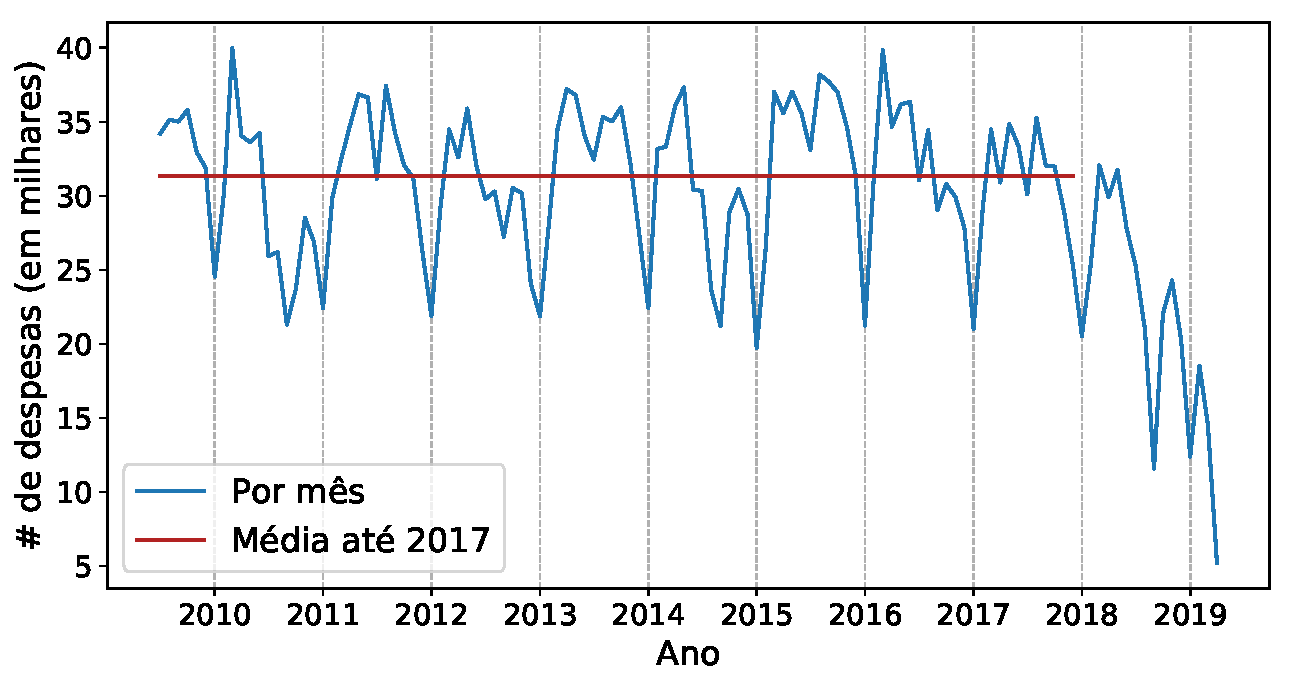
\includegraphics[width=1.0\textwidth]{graficos/n_despesas_por_mes_2019-04-29.pdf}
\caption{Número de despesas na base de dados de uso da cota parlamentar dos deputados federais
  referentes a cada mês, em função do tempo (em azul).
  A linha vermelha indica o número médio de 2009 a 2018.}
\label{fig:n-despesas-por-mes}
\end{figure} 

Para acompanhar o valor total gasto com a cota parlamentar ao longo do tempo, nós primeiro deflacionamos os
valores pelo IPCA e em seguida o decompusemos num modelo aditivo com termos de tendência geral, sazonalidade e
resíduo (veja a Fig. \ref{fig:total-despesas-por-mes}). Através da curva de tendência, podemos notar que
o valor médio gasto praticamente não se alterou desde 2010, sendo que uma leve queda pode ser notada em anos
recentes. Ressaltamos que ao menos parte dessa queda é consequência da defasagem de registro dos gastos.

\begin{figure}[H]
\centering
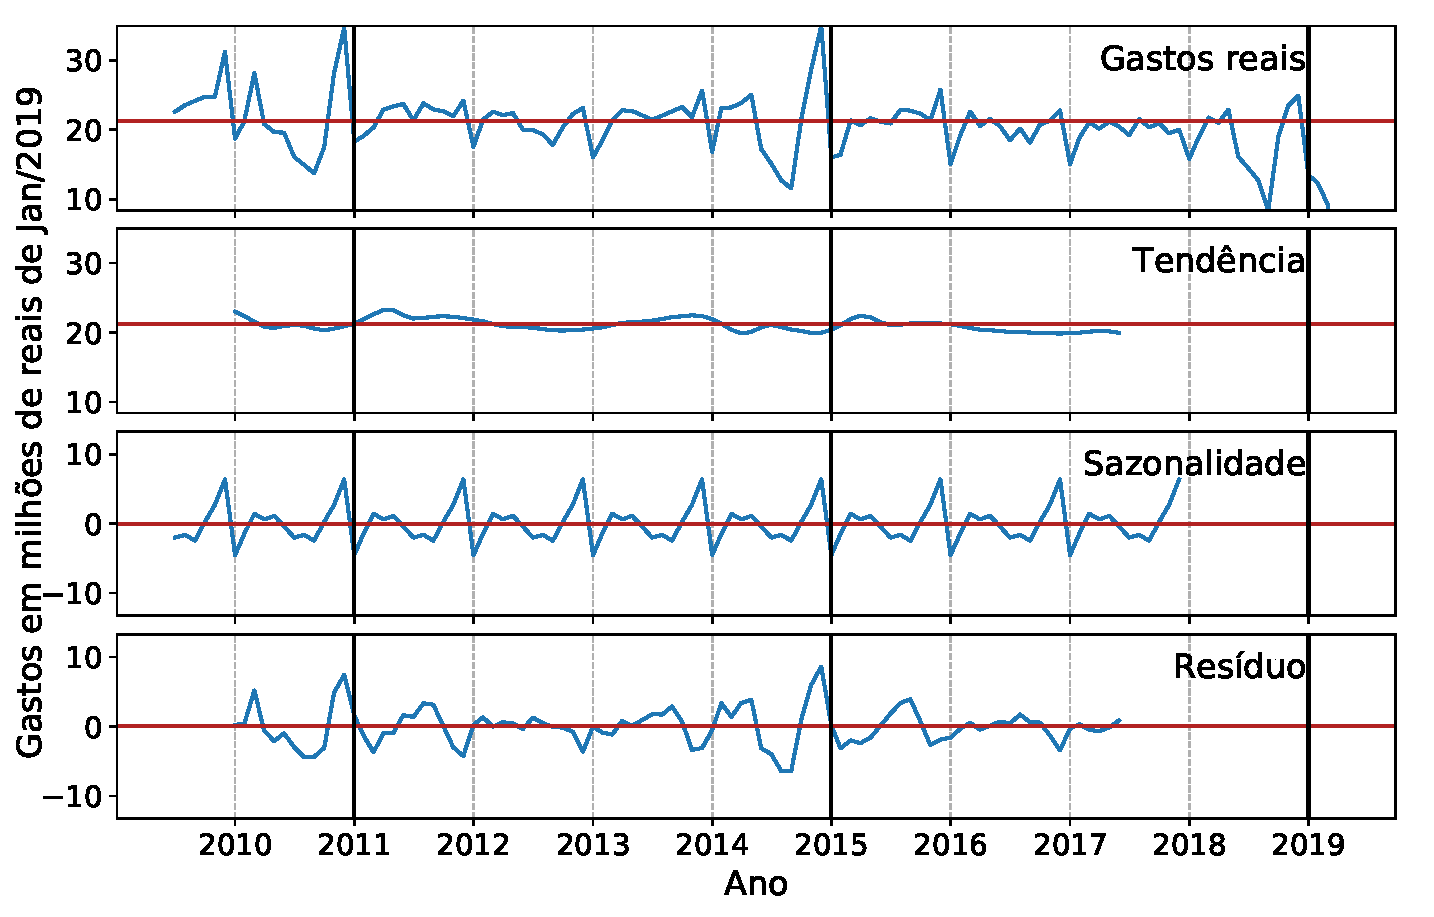
\includegraphics[width=1.0\textwidth]{graficos/despesas-reais-e-sazonalidade_2019-04-29.pdf}
\caption{Valor real (descontada a inflação) gasto com o exercício da atividade parlamentar em cada mês
  (reembolsos feitos dentro da cota parlamentar, em azul). O painel superior mostra o valor observado, e os
  abaixo mostram as contribuições de: tendência geral, calculada através de uma média móvel; sazonalidade; e resíduo.
  A linha vermelha indica o valor médio em todo o período (nos dois painéis superiores) e o zero (nos dois
  painéis inferiores). A decomposição em contribuições aditivas foi feita até o ano de 2017.}
\label{fig:total-despesas-por-mes}
\end{figure} 

Também é possível notar que os gastos apresentam uma sazonalidade bastante marcada, com quedas mais
acentuadas em janeiro e picos em dezembro. Esses picos podem decorrer do fato de que a cota parlamentar, mensal,
pode ser acumulada ao longo do ano mas não pode ser transferida para o exercício financeiro seguinte.
É possível percebem ainda, tanto nos gráficos do valor observado quanto no de resíduos, que existe
um pico ainda mais acentuado ao final de cada legislatura (marcadas com linhas verticais pretas contínuas).
Esse pico parece ser precedido por uma queda nos gastos, possivelmente indicando uma estratégia de acúmulo de verba
para a realização de um último gasto em dezembro.

Por fim, verificamos como o valor total reembolsado pela cota parlamentar se divide nas categorias pré-definidas
pela câmara. A Figura \ref{fig:despesas-por-tipo} mostra a fração do valor total que é destinada a cada categoria
de gastos. Verificamos que os maiores gastos realizados são com divulgação da atividade parlamentar (que, em geral,
apresentam valores altos para uma única despesa e perfazem 20\% do total) e com transporte aéreo: somando as rubricas
``emissão de bilhere aéreo'', ``locação ou fretamento de aeronaves'' e ``passagens aéreas'', temos cerca de
23\% dos gastos. Em grande medida, esse montante deriva do deslocamento semanal do deputado ao seu estado de origem.
Gastos com manutenção de escritório de apoio em seu estado, consultorias, telefonia e transportes terrestres vêm
em seguida. Junto com passagens aéreas, o transporte totaliza cerca de 44\% do total. Gastos com alimentação e
hospedagem fora do distrito federal totalizam, em média, menos de 2\% dos gastos.

\begin{figure}[H]
\centering
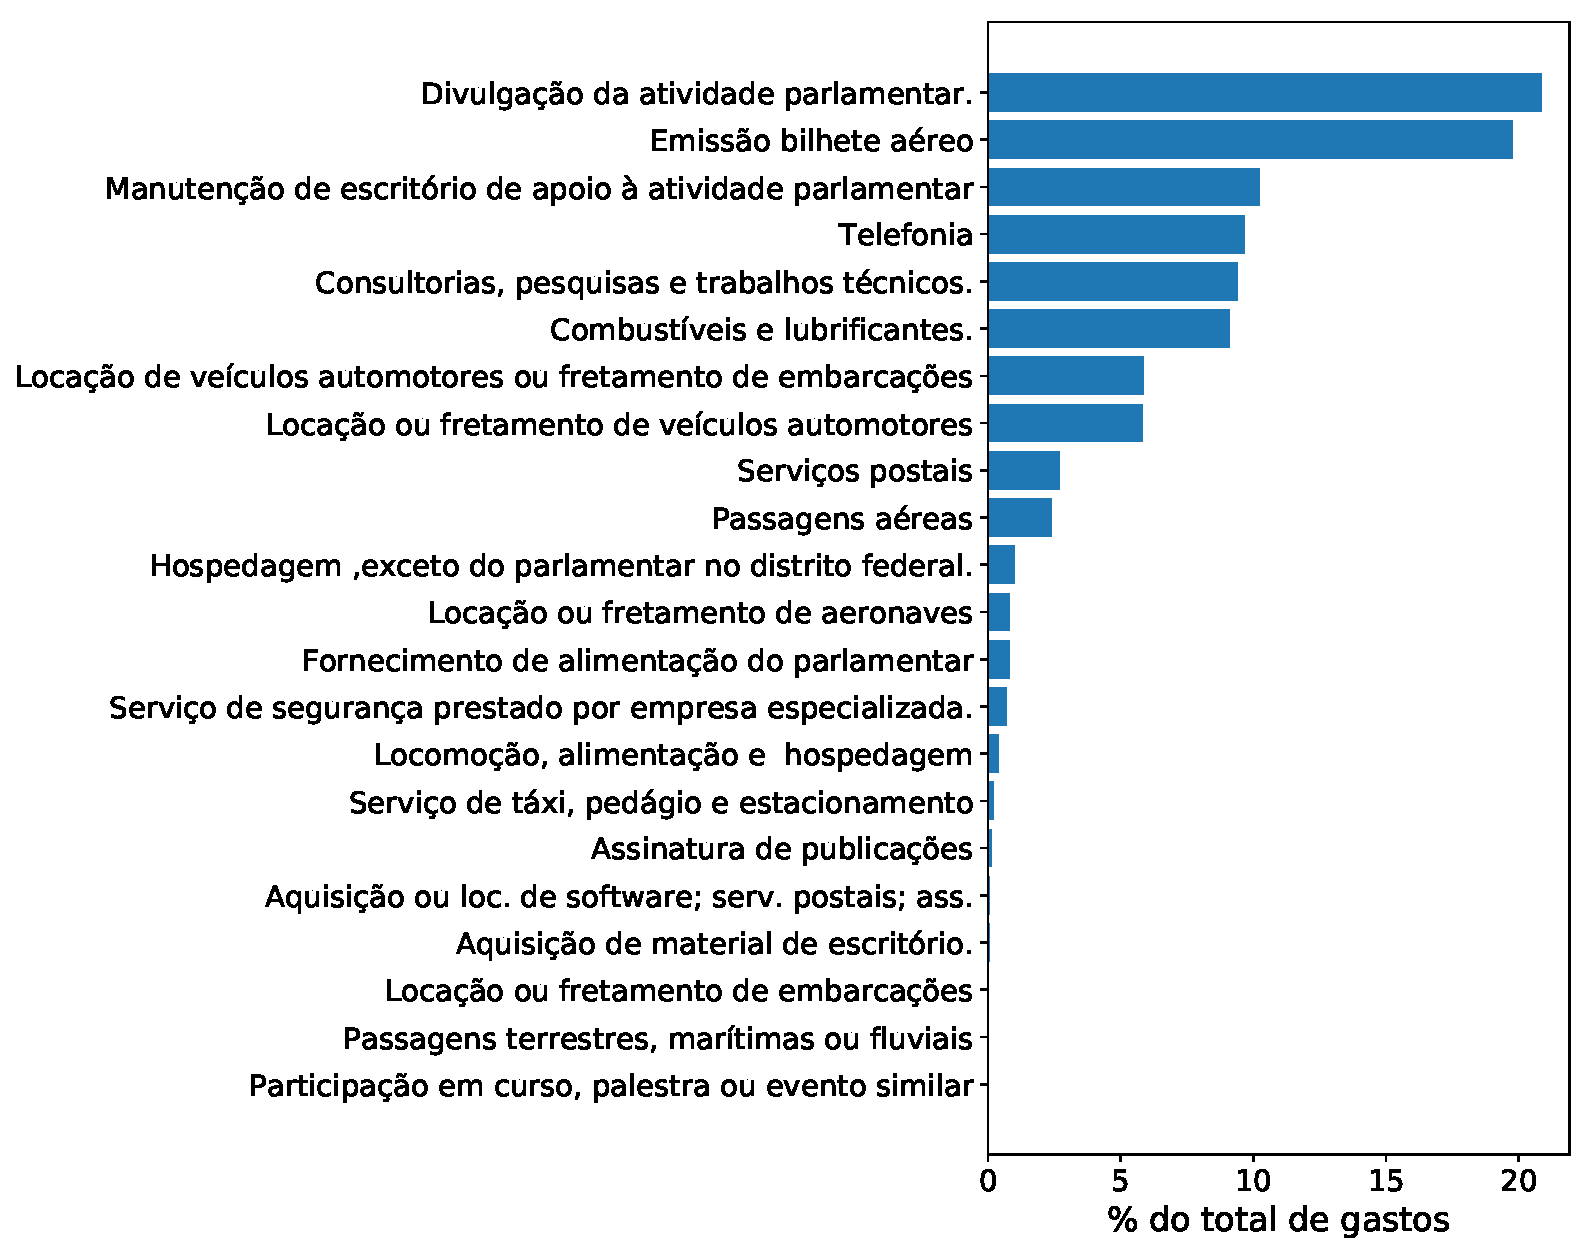
\includegraphics[width=1.0\textwidth]{graficos/total-despesas-por-tipo_2019-04-29.pdf}
\caption{Porcentagem do valor total utilizado pelos deputados federais que é destinado a cada finalidade. Nesse
cálculo, utilizamos os valores de 2009 a 2017, corrigigos pela inflação.}
\label{fig:despesas-por-tipo}
\end{figure} 



%%%%%%%%%%%%%%%%%%%%%%%%%%
\section{Proposições}
\label{sec:proposicoes}

\subsection{Câmara dos deputados}
\label{sec:temas-camara}

A base de dados abertos da câmara federal indica que, nos 100 primeiros dias da atual legislatura,
foram apresentados pouco mais de 1600 projetos de lei (PLs, veja a Fig. \ref{fig:prop-2019-tipo}),
o que resulta em, aproximadamente, 3,2 projetos por deputado. Dado que os PLs são a ampla maioria
das proposições apresentadas na legislatura atual, vamos focar nossa análise nesse tipo de proposição e
compará-las com os anos anteriores.

\begin{figure}[H]
\centering
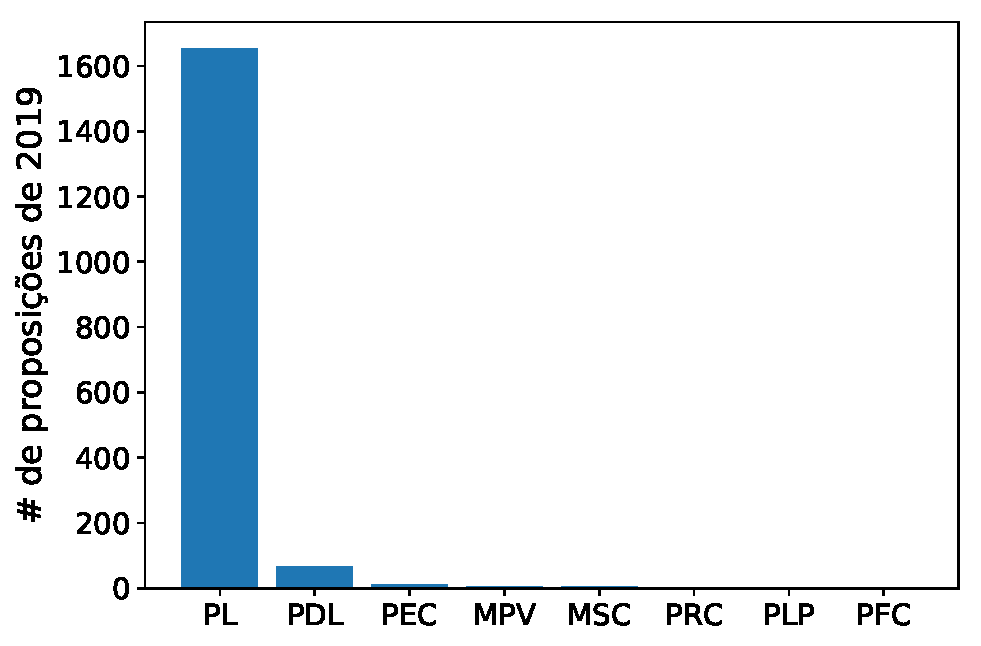
\includegraphics[width=0.7\textwidth]{graficos/proposicoes-2019-por-tipo_2019-05-01.pdf}
\caption{Número de proposições apresentadas na $56^{\mathrm{\underline{a}}}$ (atual) legislatura,
  classificadas por tipo: Projeto de Lei (PL), Projeto de Decreto Legislativo (PDL),
  Proposta de Emenda à Constituição (PEC), Medida Provisória (MPV), Mensagem de Acordos,
  convênios, tratados e atos internacionais (MSC), Projeto de Resolução da Câmara dos Deputados (PRC),
  Projeto de Lei Complementar (PLP) e Proposta de Fiscalização e Controle (PFC).}
\label{fig:prop-2019-tipo}
\end{figure} 

A Fig. \ref{fig:prop-por-ano} mostra a evolução do número de PLs apresentados ao longo do tempo,
tomando como referência o mesmo período a cada ano. Além do crescimento observado, é interessante
notar que os inícios de legislatura apresentam picos de apresentação de PLs.

\begin{figure}[H]
  \centering
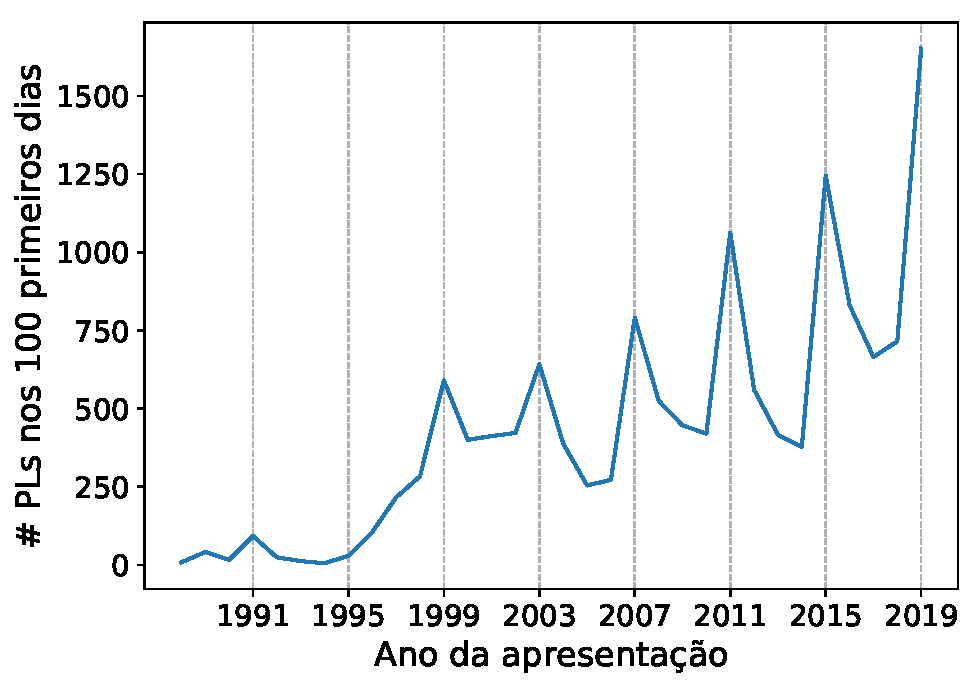
\includegraphics[width=0.7\textwidth]{graficos/PLs-por-ano_2019-05-03.pdf}
\caption{Evolução do número de PLs apresentados nos 100 dias a partir de 1 de fevereiro, de cada ano.
Os inícios de legislatura são marcados pelas linhas tracejadas cinzas.}
\label{fig:prop-por-ano}
\end{figure}

O Centro de Documentação e Informação da Câmara fornece uma classificação oficial em temas para as
proposições.\footnote{Conforme descrito em \footurl{https://dadosabertos.camara.leg.br/swagger/api.html}}
Nós verificamos a frequência com que cada tema apareceu em cada ano, de maneira que podemos saber
quais são os temas historicamente mais recorrentes nos projetos de lei e quais os temas mais em voga
na legislatura atual. A Fig. \ref{fig:pl-por-tema-camara} sintetiza os resultados, na qual comparamos
a frequência de cada tema nos projetos de lei apresentados nos 100 primeiros dias da atual legislatura com as médias das frequências
em todo o período de janeiro de 2011 a dezembro de
2018.\footnote{Uma versão simplificada desse gráfico é apresentada na Fig. \ref{fig:pl-por-tema-camara-simples}.}

A escolha desse período como referência
visa reduzir flutuações estatísticas (em comparação com intervalos menores de tempo) e evitar mudanças 
de comportamento abruptas e não plenamente entendidas que parecem ter ocorrido na passagem de 2010 a 2011
(conforme apresentamos abaixo). Além disso, verificamos não existir uma sazonalidade significativa
que justifique restringir o cálculo da média histórica aos 100 primeiros dias das legislaturas anteriores.

\begin{figure}[H]
\centering
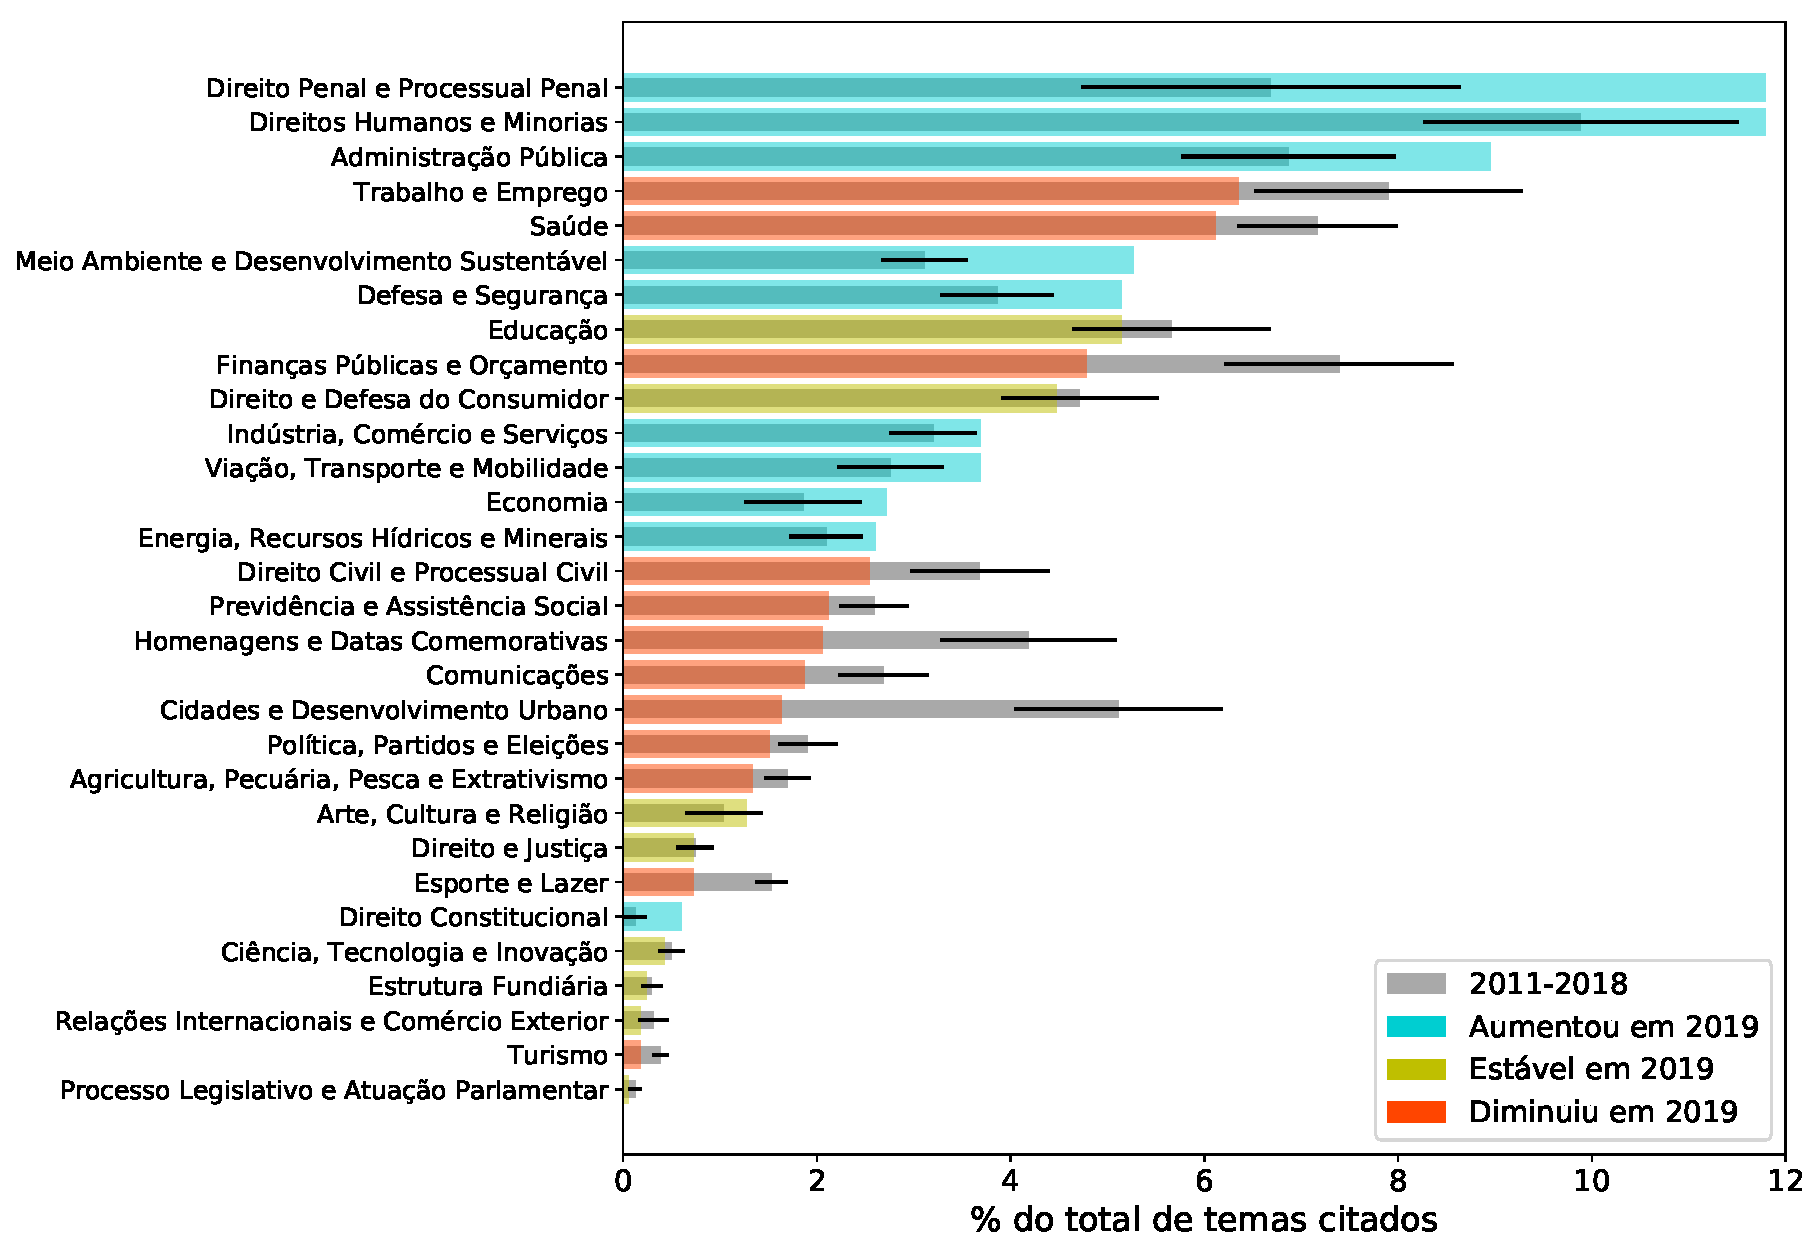
\includegraphics[width=1.0\textwidth]{graficos/temas_PL_fracao2019-vs-mediaAnterior_2019-05-03.pdf}
\caption{Frequência de cada tema (fração dos PLs apresentados que foram classificados naquele tema) na câmara.
  As barras cinzas e mais estreitas representam a média da frequência no período de janeiro de 2011 a
  dezembro de 2018, e as linhas pretas indicam a variação típica (desvio padrão) da frequência no período.
  As barras coloridas representam a frequência de cada tema para os 100 dias da atual legislatura.
  Frequências que cresceram mais que a variação típica dos anos anteriores estão em azul, e as que
  diminuíram mais que a variação típica estão em vermelho. As demais são apresentadas em amarelo.
  Os temas foram ordenados pela frequência atual.}
\label{fig:pl-por-tema-camara}
\end{figure}

Podemos notar que certos temas são, historicamente, mais frequentes que outros. No período desde 2011,
os três temas mais recorrentes foram de direitos humanos e minorias (10\%), trabalho e emprego (8\%)
e finanças públicas (7\%). Processo legislativo e atuação parlamentar, por outro lado, é tema de 0,1\%
dos PLs. Já na legislatura atual, os três temas mais comuns foram: direito penal e processual penal (12\%),
direitos humanos e minorias (12\%) e administração pública (9\%). Embora também fossem comuns nos anos
anteriores, esses temas sofreram alta, com destaque para a de direito penal e processual penal.

Os três temas que sofreram altas mais significativas foram: meio ambiente e desenvolvimento
sustentável (4,8$\sigma$, onde $\sigma$ é o desvio padrão da frequência de 2011 a 2018),
direito constitucional (4,2$\sigma$) e direito processual e penal (2,6$\sigma$). Os três
temas com baixas mais significativas foram: esporte e lazer (-4,9$\sigma$), cidades e desenvolvimento
urbano (-3,23$\sigma$) e turismo (-2,3$\sigma$). Hipotetizamos que as altas significativas
na fração de PLs apresentados indicam que os deputados estão buscando mudar as regras de jogo dentro
daquele tema em particular ou que aquele tema é prioridade para os membros da legislatura atual.
Baixas significativas podem indicar que as regras de jogo para aquele
tema são consideradas adequadas ou que o tema em questão não é prioridade para os deputados.

Conforme mencionado anteriormente, o ano de 2011 (que é um ano de início de legislatura)
marca uma mudança abrupta de comportamento para alguns temas. A Fig. \ref{fig:pl-agricultura}
exemplifica esse cenário: o tema ``estrutura fundiária'' passa de uma frequência de 2\% para outra
próxima de zero; já o tema ``Agricultura, Pecuária, Pesca e Extrativismo'' faz o caminho contrário.
Outros temas realizam transições semelhantes: direito e defesa do consumidor, direito e justiça, e
política, partidos e eleições também pulam de patamar em 2011; enquanto que viação, transporte e
mobilidade cai. Esses saltos podem indicar uma mudança na metodologia de classificação dos PLs.

\begin{figure}[H]
\centering
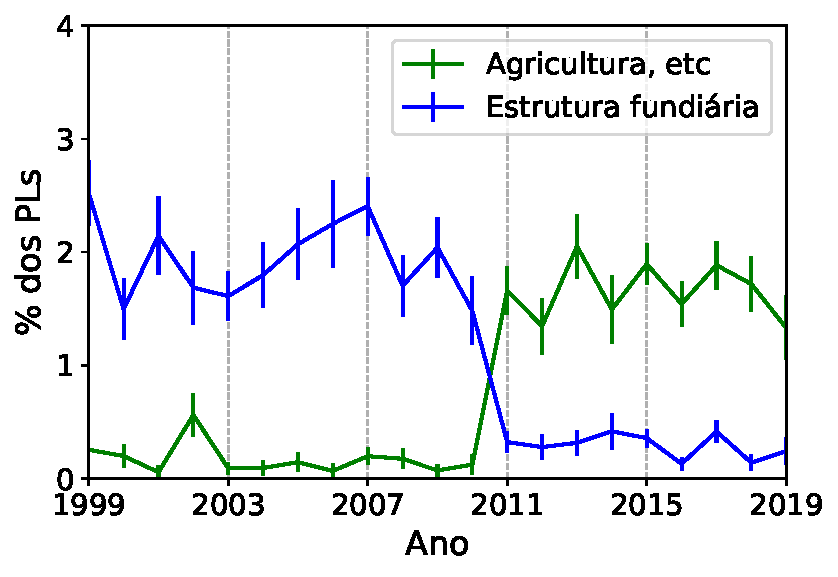
\includegraphics[width=0.6\textwidth]{graficos/PL-agricultura-por-ano_2019-05-01.pdf}
\caption{Evolução da frequência de PLs que tratam dos temas ``Agricultura, Pecuária, Pesca e Extrativismo''
  (em verde) e ``Estrutura fundiária'' (em azul), de 1999 a 2019. As barras de erro foram estimadas
assumindo que as contagems de PLs (dentro de um dado tema e de maneira agregada) sofrem flutuações de Poisson.}
\label{fig:pl-agricultura}
\end{figure}

Por fim, um achado interessante é a evolução da frequência do tema ``direitos humanos e minorias'' que,
no período analisado (de 1999 a 2019), passou por um crescimento significativo e substancial.
A Fig. \ref{fig:pl-direitos-humanos} mostra que, em 20 anos, esse tema dobrou de frequência, passando de
5\% para cerca de 11\%.

\begin{figure}[H]
\centering
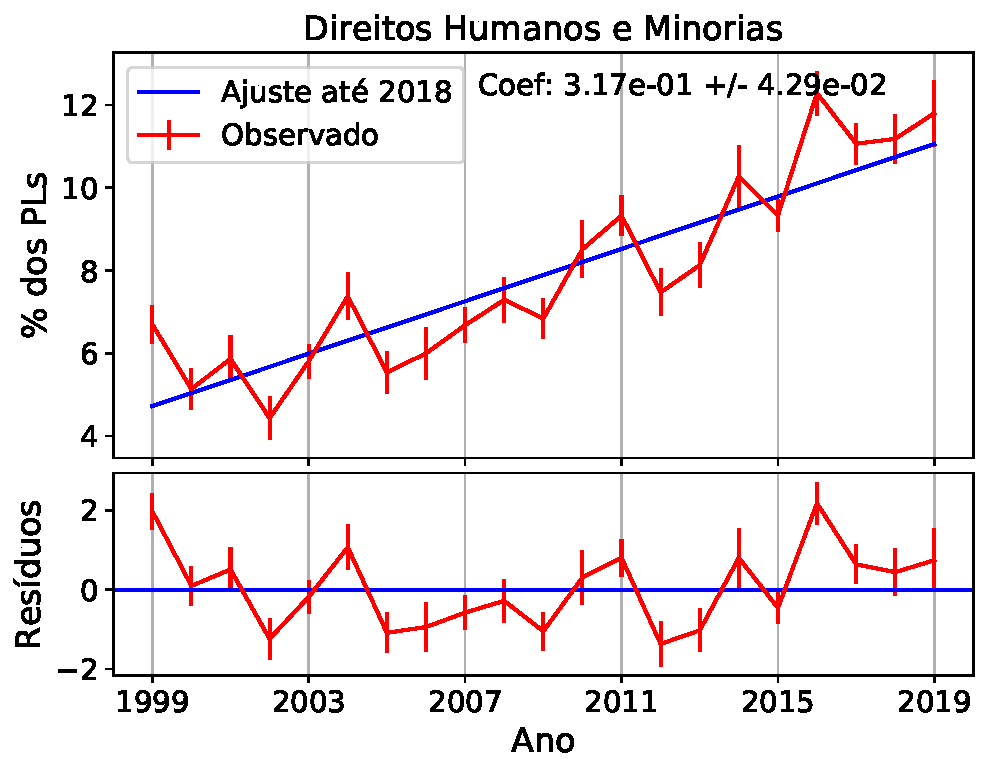
\includegraphics[width=0.7\textwidth]{graficos/PL-direitos-humanos-por-ano_2019-05-01.pdf}
\caption{O painel superior apresenta a evolução da frequência do tema ``direitos humanos e minorias''
  dentre os PLs apresentados; a linha vermelha mostra os valores observados, enquanto que a linha
  azul indica um ajuste linear com coeficiente angular $0,317\pm 0,043$. O painel inferior apresenta
  a diferença entre os valores observados e ajustados. As barras de erro foram estimadas assumindo
  flutuações de Poisson nas contagens de PLs.}
\label{fig:pl-direitos-humanos}
\end{figure}

\subsection{Senado}
\label{sec:temas-senado}

No senado, também houve record de apresentação de PLs. Foram apresentados 422 PLs nos 100 primeiros dias da legislatura 56 contra 312 da legisltura 51 que era o último recorde. Um aumento de 35\% do recorde anterior e de 53\% em relacão a legislatura anterior (Figura \ref{fig:pl-total-senado}. Nota-se também um comportamento sazonal na apresentação de proposições, aumento no primeiro ano da legislatura e subsequente diminuição nos próximos anos. Porém, o ano de 2018 foi atípico com um aumento não esperado de apresentações de PL exatamente no último ano da legislatura, no qual se tem usualmente o menor número de PLs novos.

Assim como na Câmara, a Figura \ref{fig:pl-por-tipo-senado} representa o maior número de proposições legislativas. Ignorando os Requerimentos, que são meramente processuais, as PLs vem seguidas da PEC, PRS e PDL.

\begin{figure}[H]
\centering
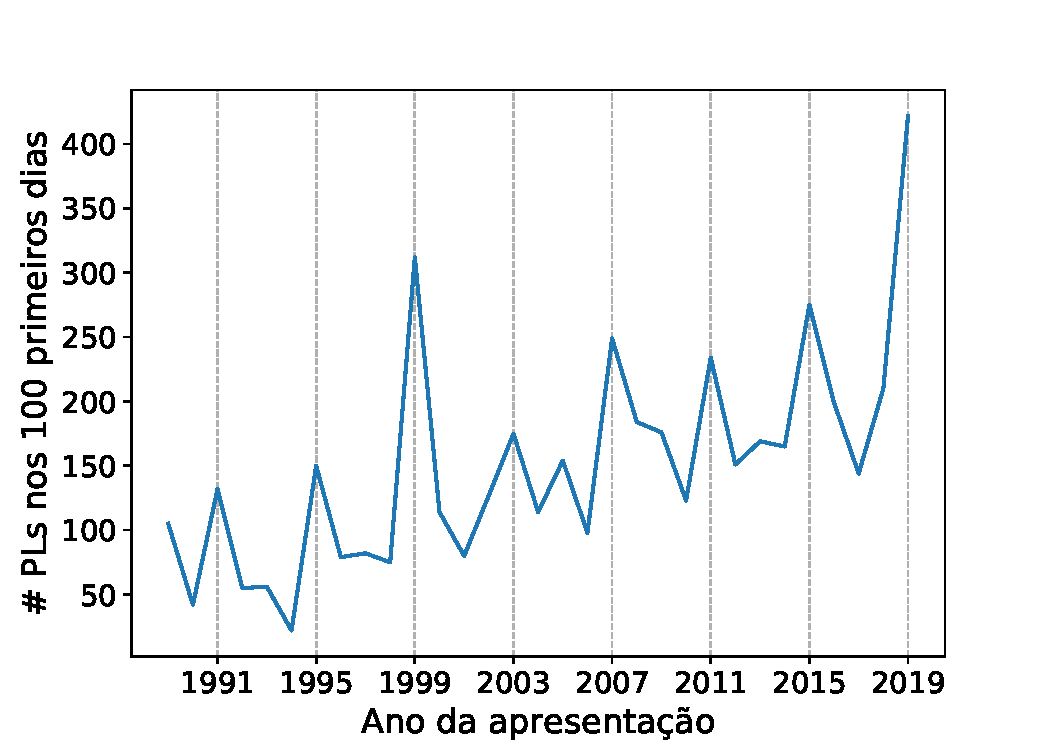
\includegraphics[width=1.0\textwidth]{graficos/senado/PLs-por-ano.pdf}
\caption{Evolução do número de PLs apresentados no Senado nos 100 dias a partir de 1 de fevereiro, década ano. Os inícios de legislatura são marcados pelas linhas tracejadas cinzas.}
\label{fig:pl-total-senado}
\end{figure}


\begin{figure}[H]
\centering
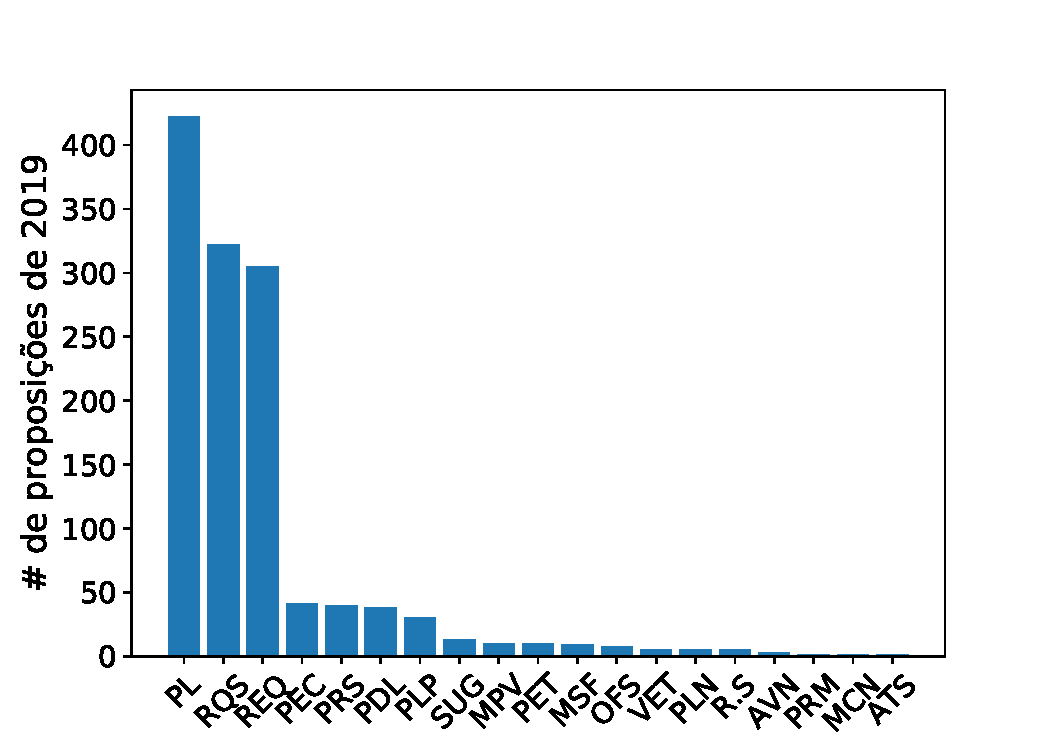
\includegraphics[width=1.0\textwidth]{graficos/senado/proposicoes-2019-por-tipo.pdf}
\caption{Número de proposições apresentadas na $56^{\mathrm{\underline{a}}}$ (atual) legislatura.}
\label{fig:pl-por-tipo-senado}
\end{figure}




\begin{tabular}{lrr}
\toprule
 &   PEC &     PL \\
ano  &       &        \\
\midrule
1988 &   0.0 &   20.0 \\
1991 &  11.0 &  132.0 \\
1995 &  32.0 &  150.0 \\
1999 &  38.0 &  312.0 \\
2003 &  33.0 &  175.0 \\
2007 &  39.0 &  249.0 \\
2011 &  32.0 &  234.0 \\
2015 &  53.0 &  275.0 \\
2019 &  41.0 &  422.0 \\
\bottomrule
\end{tabular}



A base de dados abertos do senado também classifica as proposições por temas, apesar dos temas serem
ligeiramente diferentes. A Fig. \ref{fig:pl-por-tema-senado} é análoga à Fig. \ref{fig:pl-por-tema-camara}, mas trata dos PLs apresentados
no senado.\footnote{Uma versão simplificada desse gráfico é apresentada na Fig. \ref{fig:pl-por-tema-senado-simples}.}


\begin{figure}[H]
\centering
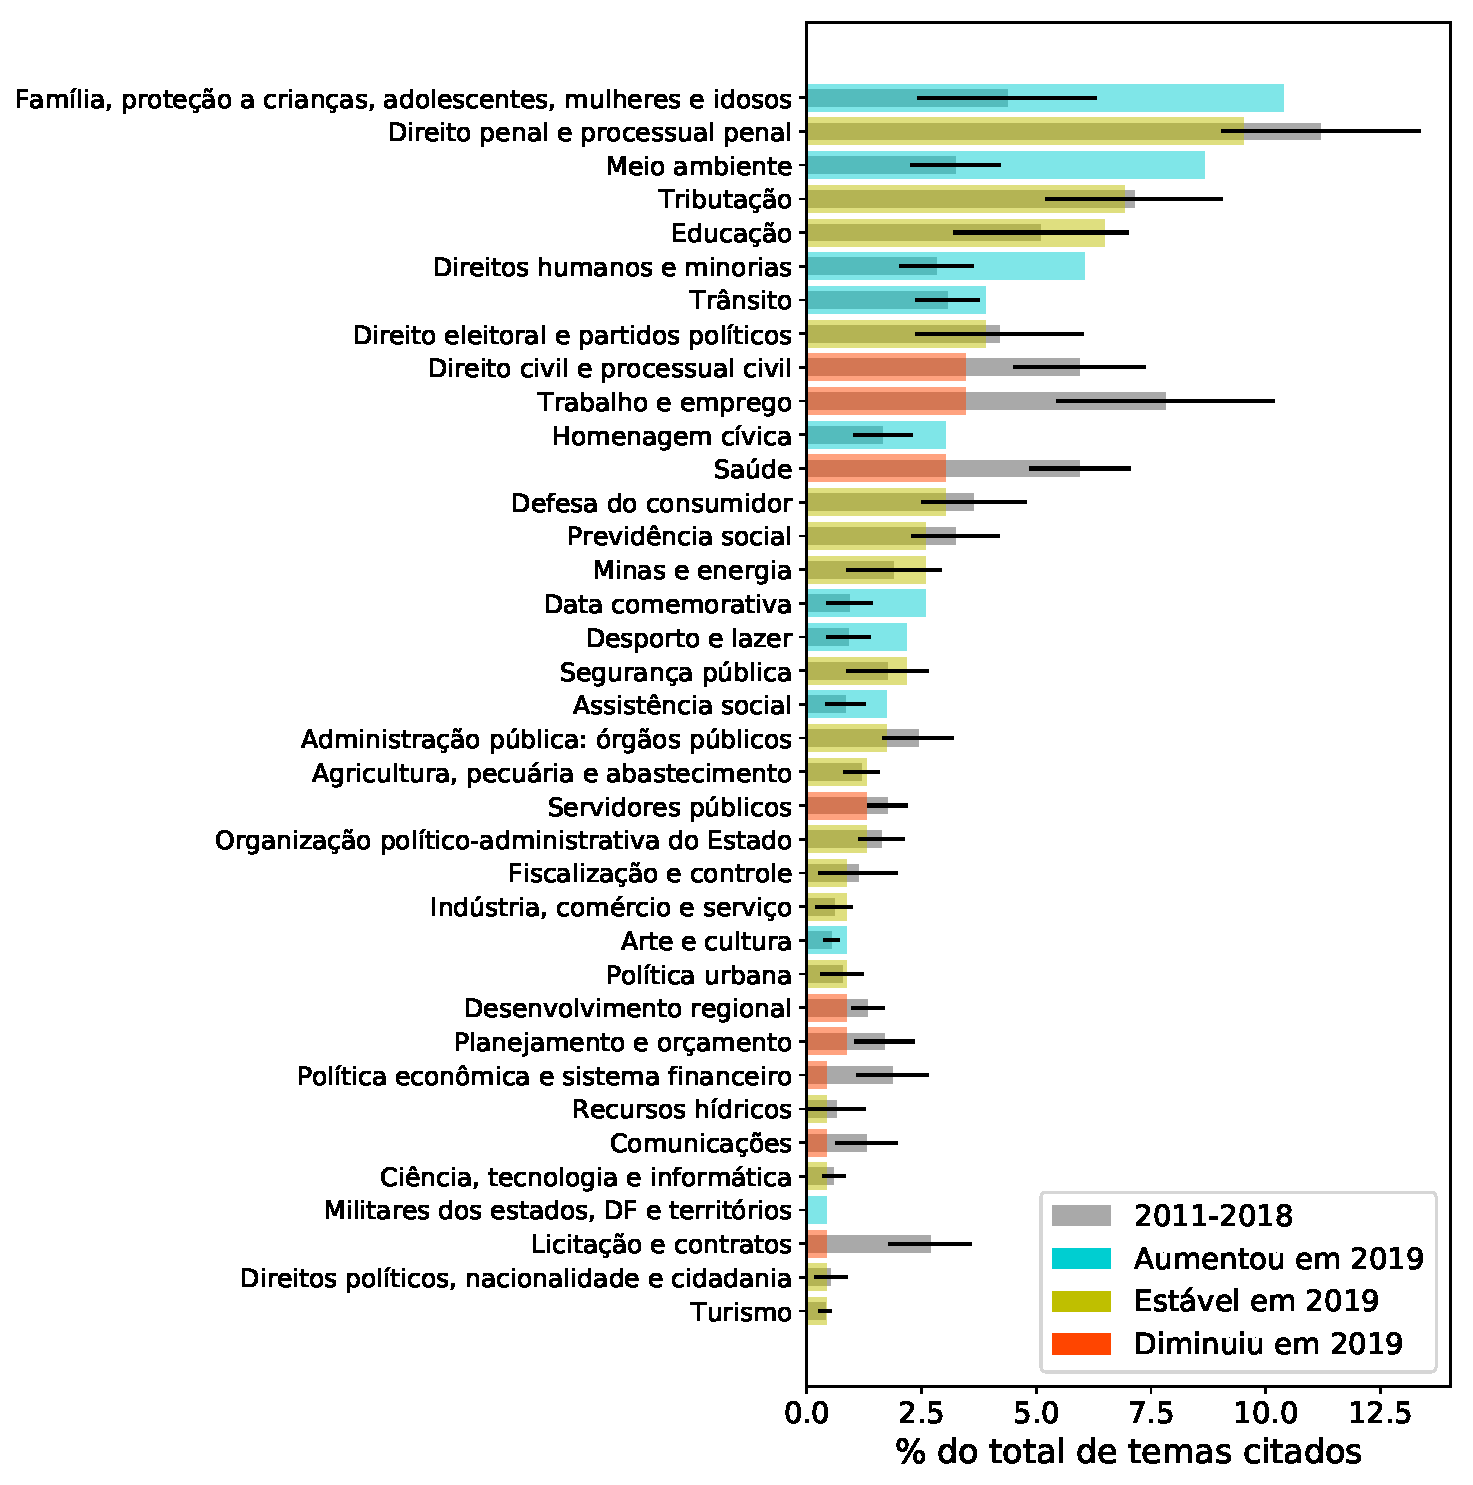
\includegraphics[width=1.0\textwidth]{graficos/senado/pls-temas-senado-r-completo.pdf}
\caption{Frequência de cada tema (fração dos PLs apresentados que foram classificados
  naquele tema) no senado. A representação e a forma de calcular a média histórica são iguais
  aos da Fig. \ref{fig:pl-por-tema-camara}.}
\label{fig:pl-por-tema-senado}
\end{figure}

Aqui, vemos algumas semelhanças à configuração de temas da câmara: os temas mais comuns são
próximos (direito penal e processual penal, direitos humanos e minorias e meio ambiente), e
também contrastam com temas como turismo e ciência e tecnologia (com baixa frequência).
As altas em 2019 dos temas ``meio ambiente'' e ``direitos humanos e minorias'' também aparecem,
enquanto que a de ``direito penal e processual penal'', não. Também notamos a repetição dos
padrões de queda nos temas ``trabalho e emprego'' e ``saúde''.
A base de dados abertos do senado também classifica as proposições em macro-temas, e suas frequências
históricas e em 2019 são apresentadas na Fig. \ref{fig:pl-por-macrotema-senado}.

\begin{figure}[H]
\centering
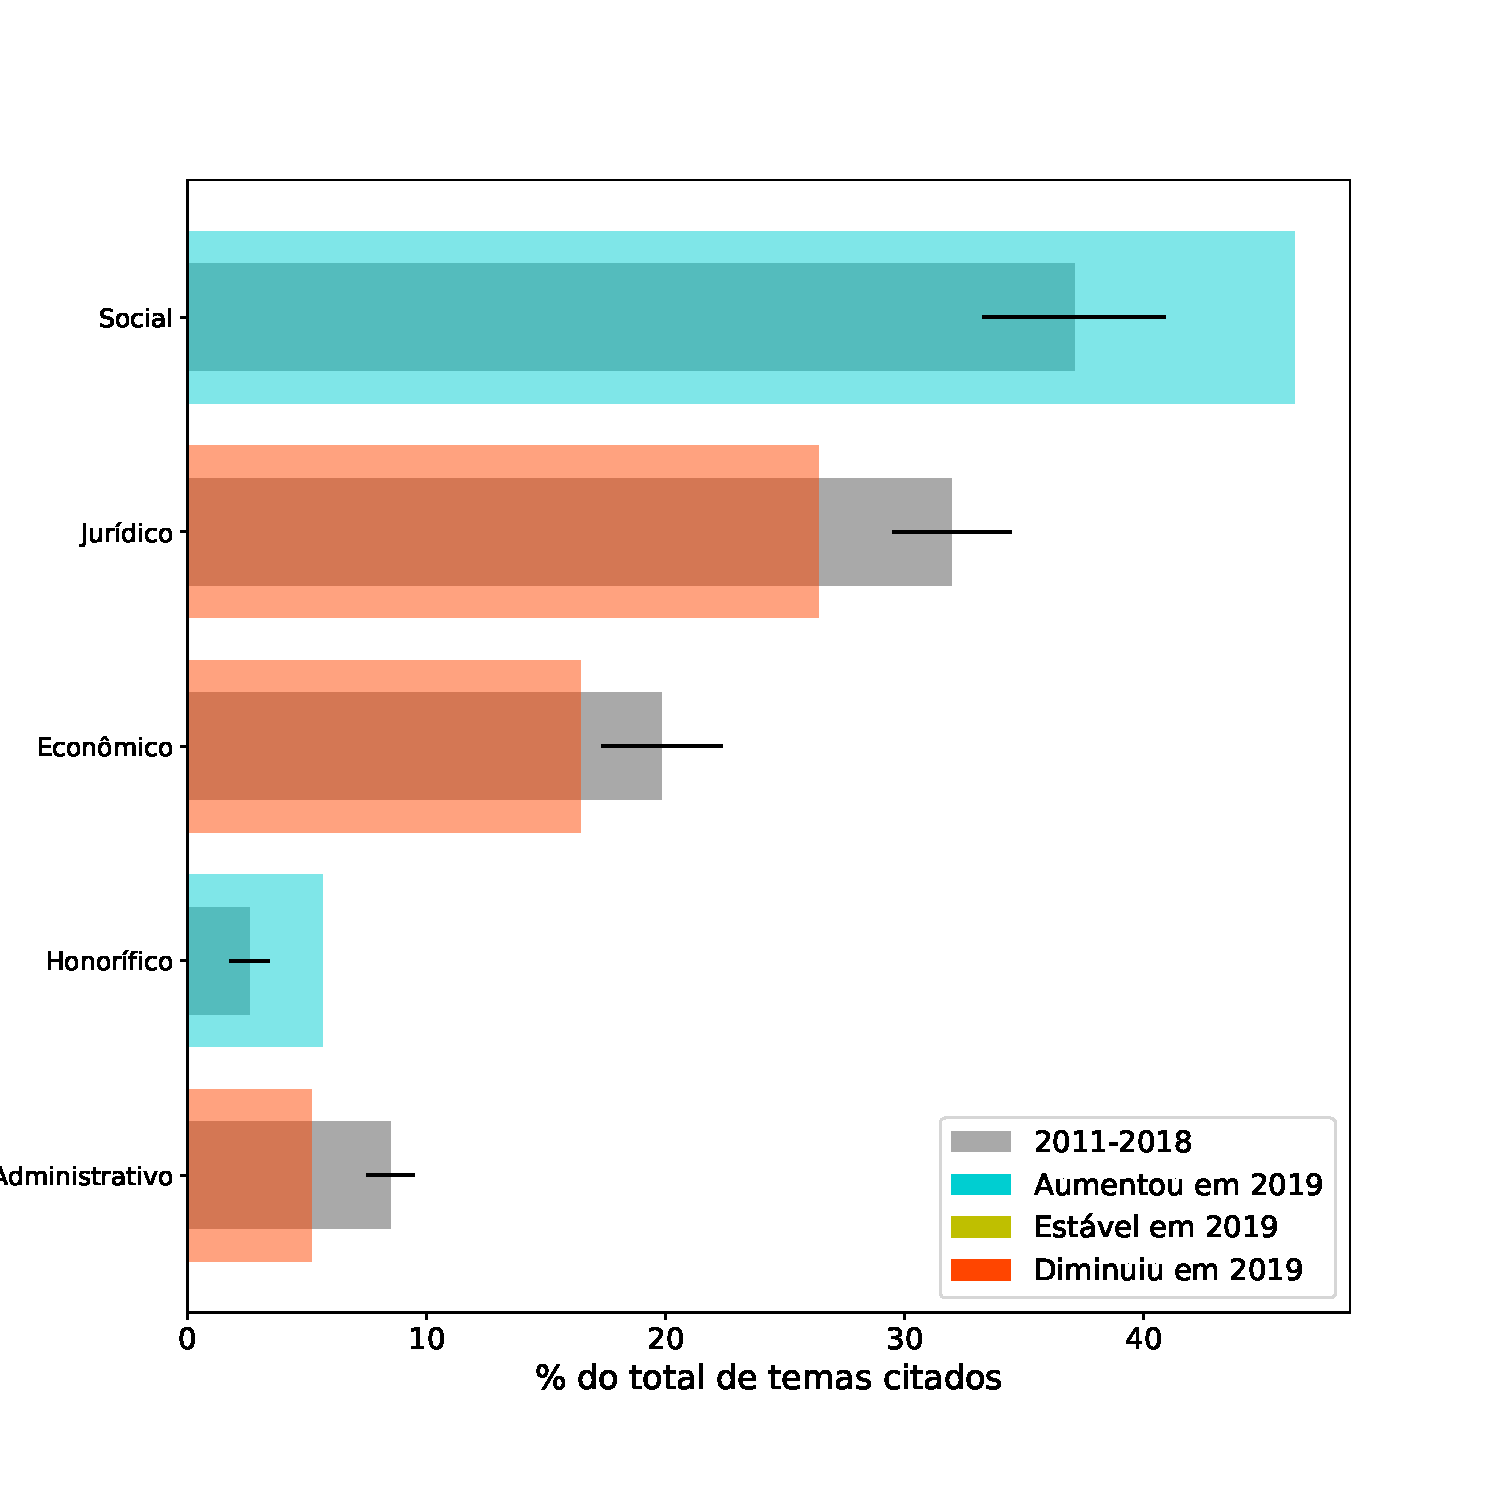
\includegraphics[width=0.7\textwidth]{graficos/senado/pls-macro-temas-senado-r-completo.pdf}
\caption{Frequência de cada macro-tema (fração dos PLs apresentados que foram classificados
  naquele macro-tema) no senado. A representação e a forma de calcular a média histórica são iguais
  aos da Fig. \ref{fig:pl-por-tema-camara}.}
\label{fig:pl-por-macrotema-senado}
\end{figure}

%\HX{Incluir tabela com dados sobre temas}

%%%%%%%%%%%%%%%%%%%%%%%%%%%%
\section{Tabelas}
\pagestyle{final}
\label{sec:tabelas}
Nesta seção, listamos tabelas que contém as informações apresentadas em alguns gráficos do relatório.

{\footnotesize
\begin{longtable}{llrrr}
    \caption{Lista de deputados da atual legislatura, junto com seu último partido, a fração de votos
  alinhados com o governo, o número de votações com orientações dadas pelo partido no qual o deputado participou,
  e a fração de votos alinhados com o partido. No período em questão, houve 53 votações, sendo que o
  governo orientou o voto em 33 delas.}\\

\toprule
                                Nome &        Partido &  Al. gov. &  \# Or. part. &  Al. part. \\
                                     &                &           &              &            \\
\midrule
\endhead
\midrule
\multicolumn{5}{r}{{Continua na próxima página}} \\
\midrule
\endfoot

\bottomrule
\endlastfoot
                       André Janones &         Avante &      56,7 &            8 &       87,5 \\
                    Chiquinho Brazão &         Avante &      82,1 &            5 &       80,0 \\
                        Greyce Elias &         Avante &      77,4 &            7 &       57,1 \\
                         Leda Sadala &         Avante &      52,9 &            1 &      100,0 \\
                           Luis Tibé &         Avante &     100,0 &            5 &       60,0 \\
            Pastor Sargento Isidório &         Avante &      25,0 &            5 &       40,0 \\
                                Tito &         Avante &      68,8 &            8 &       62,5 \\
                        Alex Manente &      Cidadania &     100,0 &           43 &       95,3 \\
                      Arnaldo Jardim &      Cidadania &      96,9 &           46 &       95,7 \\
                      Carmen Zanotto &      Cidadania &     100,0 &           46 &       97,8 \\
                          Da Vitória &      Cidadania &      93,8 &           47 &       95,7 \\
                       Daniel Coelho &      Cidadania &     100,0 &           41 &      100,0 \\
                      Marcelo Calero &      Cidadania &      97,0 &           51 &       94,1 \\
                      Paula Belmonte &      Cidadania &     100,0 &           45 &       97,8 \\
                        Rubens Bueno &      Cidadania &     100,0 &           49 &      100,0 \\
                           Alan Rick &            DEM &     100,0 &            9 &      100,0 \\
                     Alexandre Leite &            DEM &     100,0 &            9 &      100,0 \\
                Arthur Oliveira Maia &            DEM &     100,0 &           10 &      100,0 \\
                         Bilac Pinto &            DEM &     100,0 &            4 &      100,0 \\
              Carlos Henrique Gaguim &            DEM &      93,9 &           10 &       90,0 \\
                        David Soares &            DEM &      93,3 &            1 &      100,0 \\
                 Dr. Zacharias Calil &            DEM &     100,0 &            9 &      100,0 \\
                        Efraim Filho &            DEM &     100,0 &            6 &      100,0 \\
                    Eli Corrêa Filho &            DEM &     100,0 &            5 &      100,0 \\
                    Elmar Nascimento &            DEM &     100,0 &            2 &      100,0 \\
               Fernando Coelho Filho &            DEM &     100,0 &            0 &          - \\
                     Geninho Zuliani &            DEM &     100,0 &            6 &      100,0 \\
                         Hélio Leite &            DEM &     100,0 &           10 &      100,0 \\
                Jose Mario Schreiner &            DEM &     100,0 &           10 &      100,0 \\
                     Juninho do Pneu &            DEM &      96,9 &            9 &      100,0 \\
                     Juscelino Filho &            DEM &     100,0 &            9 &      100,0 \\
                       Kim Kataguiri &            DEM &      96,6 &            6 &      100,0 \\
                 Leur Lomanto Júnior &            DEM &     100,0 &            9 &      100,0 \\
                        Luis Miranda &            DEM &     100,0 &            1 &        0,0 \\
                          Norma Ayub &            DEM &     100,0 &           10 &      100,0 \\
                      Olival Marques &            DEM &     100,0 &            9 &      100,0 \\
                           Paulo Azi &            DEM &     100,0 &           10 &      100,0 \\
                        Pedro Lupion &            DEM &      96,6 &            9 &      100,0 \\
                         Pedro Paulo &            DEM &     100,0 &            9 &      100,0 \\
   Professora Dorinha Seabra Rezende &            DEM &      94,7 &            9 &      100,0 \\
                        Rodrigo Maia &            DEM &     100,0 &            0 &          - \\
                 Sóstenes Cavalcante &            DEM &      90,9 &            6 &      100,0 \\
                       Alceu Moreira &            MDB &     100,0 &            1 &      100,0 \\
                        Baleia Rossi &            MDB &      92,6 &            7 &      100,0 \\
                     Carlos Chiodini &            MDB &     100,0 &            9 &       88,9 \\
                      Celso Maldaner &            MDB &     100,0 &            8 &       87,5 \\
                 Daniela do Waguinho &            MDB &      96,9 &            9 &      100,0 \\
                    Darcísio Perondi &            MDB &     100,0 &            9 &      100,0 \\
                       Dulce Miranda &            MDB &      92,0 &            9 &       88,9 \\
                    Elcione Barbalho &            MDB &     100,0 &            9 &      100,0 \\
                          Fabio Reis &            MDB &     100,0 &           10 &      100,0 \\
                       Flaviano Melo &            MDB &      94,4 &            6 &      100,0 \\
                       Fábio Ramalho &            MDB &      93,3 &            8 &      100,0 \\
                      Giovani Feltes &            MDB &     100,0 &           10 &      100,0 \\
                      Gutemberg Reis &            MDB &      92,9 &            8 &       87,5 \\
                    Herculano Passos &            MDB &     100,0 &            6 &      100,0 \\
               Hercílio Coelho Diniz &            MDB &      92,9 &           10 &      100,0 \\
                  Hermes Parcianello &            MDB &      73,3 &           10 &      100,0 \\
                         Hildo Rocha &            MDB &      97,0 &           10 &      100,0 \\
                 Isnaldo Bulhões Jr. &            MDB &     100,0 &            4 &      100,0 \\
                        José Priante &            MDB &     100,0 &            1 &      100,0 \\
                  João Marcelo Souza &            MDB &     100,0 &           10 &      100,0 \\
                        Juarez Costa &            MDB &      90,3 &           10 &      100,0 \\
                       Jéssica Sales &            MDB &      92,6 &            9 &      100,0 \\
                      Lucio Mosquini &            MDB &      81,5 &            7 &      100,0 \\
              Marcos Aurélio Sampaio &            MDB &     100,0 &           10 &      100,0 \\
                         Mauro Lopes &            MDB &     100,0 &            1 &      100,0 \\
                     Moses Rodrigues &            MDB &     100,0 &            7 &      100,0 \\
                      Márcio Biolchi &            MDB &     100,0 &           10 &      100,0 \\
                   Newton Cardoso Jr &            MDB &      73,7 &            4 &       75,0 \\
                          Raul Henry &            MDB &      97,0 &           10 &      100,0 \\
            Rogério Peninha Mendonça &            MDB &      80,6 &            9 &       88,9 \\
                        Sergio Souza &            MDB &     100,0 &            7 &      100,0 \\
                    Valtenir Pereira &            MDB &      94,7 &            5 &      100,0 \\
                      Vinicius Farah &            MDB &      93,3 &            9 &      100,0 \\
                        Walter Alves &            MDB &     100,0 &           10 &      100,0 \\
                     Adriana Ventura &           NOVO &     100,0 &           49 &      100,0 \\
                     Alexis Fonteyne &           NOVO &     100,0 &           50 &      100,0 \\
                      Gilson Marques &           NOVO &     100,0 &           50 &      100,0 \\
                      Lucas Gonzalez &           NOVO &      97,0 &           49 &      100,0 \\
                   Marcel van Hattem &           NOVO &      96,9 &           46 &      100,0 \\
                        Paulo Ganime &           NOVO &      94,1 &           49 &      100,0 \\
                       Tiago Mitraud &           NOVO &      93,9 &           50 &      100,0 \\
                       Vinicius Poit &           NOVO &     100,0 &           50 &       98,0 \\
                      Alice Portugal &          PCdoB &      16,7 &           21 &      100,0 \\
                      Daniel Almeida &          PCdoB &       9,1 &           13 &      100,0 \\
                     Jandira Feghali &          PCdoB &      17,9 &           18 &      100,0 \\
                        Márcio Jerry &          PCdoB &      20,0 &           22 &       95,5 \\
                       Orlando Silva &          PCdoB &      26,1 &           18 &       94,4 \\
                    Perpétua Almeida &          PCdoB &      19,2 &           18 &      100,0 \\
               Professora Marcivania &          PCdoB &       4,3 &           16 &      100,0 \\
                   Renildo Calheiros &          PCdoB &      16,1 &           19 &      100,0 \\
               Rubens Pereira Júnior &          PCdoB &      14,3 &            0 &          - \\
                        Afonso Motta &            PDT &      45,5 &           33 &       90,9 \\
                        Alex Santana &            PDT &      56,0 &           24 &       87,5 \\
                    André Figueiredo &            PDT &      47,8 &           26 &       96,2 \\
                      Chico D`Angelo &            PDT &      23,1 &           24 &       95,8 \\
                  Dagoberto Nogueira &            PDT &      44,0 &           27 &      100,0 \\
                    Damião Feliciano &            PDT &      65,2 &           25 &       84,0 \\
                    Eduardo Bismarck &            PDT &      50,0 &           30 &       90,0 \\
                       Flávia Morais &            PDT &      60,9 &           26 &       88,5 \\
                     Flávio Nogueira &            PDT &      46,4 &           29 &      100,0 \\
                      Fábio Henrique &            PDT &      51,6 &           31 &       87,1 \\
               Félix Mendonça Júnior &            PDT &      61,9 &           23 &       95,7 \\
                          Gil Cutrim &            PDT &      57,7 &           26 &       96,2 \\
                       Gustavo Fruet &            PDT &      57,1 &           26 &       96,2 \\
                     Idilvan Alencar &            PDT &      45,2 &           31 &       93,5 \\
                        Jesus Sérgio &            PDT &      34,8 &           25 &       92,0 \\
                   Leônidas Cristino &            PDT &      32,3 &           33 &       93,9 \\
                       Marlon Santos &            PDT &      36,8 &           23 &       87,0 \\
               Mauro Benevides Filho &            PDT &      47,1 &           21 &       90,5 \\
                      Mário Heringer &            PDT &      60,0 &           12 &       91,7 \\
                         Paulo Ramos &            PDT &      38,5 &           25 &       92,0 \\
                    Pompeo de Mattos &            PDT &      50,0 &           28 &      100,0 \\
                    Robério Monteiro &            PDT &      45,5 &           33 &       93,9 \\
                      Sergio Vidigal &            PDT &      42,3 &           26 &       88,5 \\
                     Silvia Cristina &            PDT &      45,5 &           34 &       91,2 \\
                  Subtenente Gonzaga &            PDT &      66,7 &           24 &       79,2 \\
                       Tabata Amaral &            PDT &      60,9 &           23 &       87,0 \\
                       Túlio Gadêlha &            PDT &      30,8 &           27 &       92,6 \\
                      Wolney Queiroz &            PDT &      24,1 &           29 &       96,6 \\
                       Igor Kannário &            PHS &      96,9 &            4 &      100,0 \\
                         Marcelo Aro &            PHS &     100,0 &            1 &      100,0 \\
                      Eduardo Braide &            PMN &      87,5 &            1 &      100,0 \\
                   Pastor Gildenemyr &            PMN &     100,0 &            1 &      100,0 \\
                            Zé Vitor &            PMN &     100,0 &            3 &      100,0 \\
                      Abílio Santana &             PR &      83,9 &           10 &       90,0 \\
                      Altineu Côrtes &             PR &     100,0 &            9 &      100,0 \\
                         Bosco Costa &             PR &      96,8 &           11 &      100,0 \\
                     Capitão Augusto &             PR &     100,0 &           12 &       91,7 \\
                 Capitão Fábio Abreu &             PR &     100,0 &            1 &      100,0 \\
           Christiane de Souza Yared &             PR &      96,2 &           13 &      100,0 \\
                      Cristiano Vale &             PR &     100,0 &           13 &      100,0 \\
                          Dr. Jaziel &             PR &     100,0 &           13 &      100,0 \\
                          Edio Lopes &             PR &      95,8 &            7 &      100,0 \\
                    Fernando Rodolfo &             PR &      97,1 &           11 &      100,0 \\
                       Flávia Arruda &             PR &     100,0 &           10 &       90,0 \\
                      Gelson Azevedo &             PR &      97,1 &           10 &      100,0 \\
                             Giacobo &             PR &     100,0 &            9 &      100,0 \\
                     Giovani Cherini &             PR &     100,0 &           12 &      100,0 \\
               Josimar Maranhãozinho &             PR &      96,8 &            7 &      100,0 \\
                          José Rocha &             PR &     100,0 &           10 &      100,0 \\
                 João Carlos Bacelar &             PR &     100,0 &            4 &      100,0 \\
                           João Maia &             PR &     100,0 &            6 &      100,0 \\
                     Junior Lourenço &             PR &     100,0 &           11 &      100,0 \\
                         Júnior Mano &             PR &      92,3 &           14 &       92,9 \\
                            Lauriete &             PR &     100,0 &           13 &      100,0 \\
                     Lincoln Portela &             PR &     100,0 &            6 &      100,0 \\
                   Luiz Carlos Motta &             PR &     100,0 &           11 &       90,9 \\
                      Luiz Nishimori &             PR &     100,0 &            4 &      100,0 \\
                       Magda Mofatto &             PR &      88,0 &           13 &      100,0 \\
                       Marcelo Ramos &             PR &     100,0 &           12 &      100,0 \\
                       Marcio Alvino &             PR &     100,0 &           12 &       91,7 \\
                     Miguel Lombardi &             PR &     100,0 &           12 &      100,0 \\
                  Paulo Freire Costa &             PR &     100,0 &            8 &      100,0 \\
               Policial Katia Sastre &             PR &     100,0 &           10 &      100,0 \\
                      Raimundo Costa &             PR &      97,0 &           11 &      100,0 \\
                  Sebastião Oliveira &             PR &     100,0 &            9 &      100,0 \\
                       Sergio Toledo &             PR &      87,9 &           13 &      100,0 \\
                       Soraya Santos &             PR &     100,0 &            0 &          - \\
                            Tiririca &             PR &      94,1 &           12 &      100,0 \\
                   Vicentinho Júnior &             PR &     100,0 &           10 &      100,0 \\
                     Vinicius Gurgel &             PR &     100,0 &            5 &      100,0 \\
                  Wellington Roberto &             PR &      66,7 &            2 &      100,0 \\
                        Aline Gurgel &            PRB &      77,3 &           20 &       90,0 \\
                          Amaro Neto &            PRB &      88,2 &           34 &       97,1 \\
                      Aroldo Martins &            PRB &      87,5 &           34 &      100,0 \\
                      Benes Leocádio &            PRB &     100,0 &           33 &       93,9 \\
                Capitão Alberto Neto &            PRB &      97,0 &           31 &       90,3 \\
                        Carlos Gomes &            PRB &      91,2 &           32 &      100,0 \\
                    Celso Russomanno &            PRB &      72,0 &           21 &       90,5 \\
                        Cleber Verde &            PRB &     100,0 &           22 &       86,4 \\
                     Gilberto Abramo &            PRB &      84,4 &           34 &       91,2 \\
                          Hugo Motta &            PRB &      91,7 &           27 &       85,2 \\
                         Hélio Costa &            PRB &      81,2 &           31 &       96,8 \\
                   Jhonatan de Jesus &            PRB &      85,7 &           24 &      100,0 \\
                          Jorge Braz &            PRB &      81,8 &           34 &       97,1 \\
                         João Campos &            PRB &      95,0 &           18 &       88,9 \\
                           João Roma &            PRB &      93,3 &           30 &       93,3 \\
                 Julio Cesar Ribeiro &            PRB &      84,4 &           34 &       94,1 \\
                Lafayette de Andrada &            PRB &      90,3 &           29 &       89,7 \\
                      Luizão Goulart &            PRB &      76,5 &           34 &       91,2 \\
                       Manuel Marcos &            PRB &      90,3 &           34 &       97,1 \\
                      Marcos Pereira &            PRB &      84,6 &           10 &      100,0 \\
                         Maria Rosas &            PRB &      84,4 &           33 &       97,0 \\
                       Milton Vieira &            PRB &      83,9 &           31 &       96,8 \\
                      Márcio Marinho &            PRB &      66,7 &           32 &       93,8 \\
                       Ossesio Silva &            PRB &      84,4 &           34 &       97,1 \\
                       Roberto Alves &            PRB &      84,8 &           33 &       97,0 \\
                     Rosangela Gomes &            PRB &      95,5 &           19 &      100,0 \\
                     Severino Pessoa &            PRB &      64,0 &           23 &       78,3 \\
                        Silas Câmara &            PRB &      92,6 &           26 &       88,5 \\
                  Silvio Costa Filho &            PRB &      96,6 &           30 &       93,3 \\
                        Vavá Martins &            PRB &      83,3 &           31 &       93,5 \\
                   Vinicius Carvalho &            PRB &      63,6 &           20 &       90,0 \\
                      Acácio Favacho &           PROS &      93,5 &           12 &       91,7 \\
                         Boca Aberta &           PROS &      65,2 &            5 &       60,0 \\
                      Capitão Wagner &           PROS &      73,3 &           11 &      100,0 \\
                  Clarissa Garotinho &           PROS &      55,0 &            8 &       87,5 \\
                       Eros Biondini &           PROS &     100,0 &           11 &       90,9 \\
                       Gastão Vieira &           PROS &      86,4 &           11 &      100,0 \\
                  Toninho Wandscheer &           PROS &     100,0 &           10 &       90,0 \\
                     Uldurico Junior &           PROS &      66,7 &            9 &      100,0 \\
                     Vaidon Oliveira &           PROS &      81,2 &           13 &      100,0 \\
                       Weliton Prado &           PROS &      25,0 &           10 &       70,0 \\
                   Alcides Rodrigues &            PRP &     100,0 &            5 &      100,0 \\
                    Alessandro Molon &            PSB &      24,1 &           36 &      100,0 \\
                       Aliel Machado &            PSB &      40,0 &           36 &       94,4 \\
                     Bira do Pindaré &            PSB &      18,8 &           41 &       95,1 \\
                   Camilo Capiberibe &            PSB &      12,5 &           39 &       94,9 \\
                      Cássio Andrade &            PSB &      57,6 &           40 &       80,0 \\
                       Danilo Cabral &            PSB &      24,1 &           38 &       94,7 \\
                       Denis Bezerra &            PSB &      23,5 &           41 &      100,0 \\
                           Elias Vaz &            PSB &      20,0 &           39 &       92,3 \\
                    Emidinho Madeira &            PSB &      90,3 &           37 &       51,4 \\
                     Felipe Carreras &            PSB &      56,0 &           24 &       95,8 \\
                       Felipe Rigoni &            PSB &      72,4 &           34 &       64,7 \\
                       Gervásio Maia &            PSB &      36,4 &           39 &       97,4 \\
                    Gonzaga Patriota &            PSB &      50,0 &           10 &       70,0 \\
                       Heitor Schuch &            PSB &      18,2 &           27 &       96,3 \\
                    Jefferson Campos &            PSB &      71,0 &           37 &       75,7 \\
                                 Jhc &            PSB &      39,1 &           29 &       96,6 \\
                      João H. Campos &            PSB &      28,1 &           38 &       97,4 \\
                       Júlio Delgado &            PSB &      38,7 &           37 &      100,0 \\
                       Liziane Bayer &            PSB &      53,8 &           27 &      100,0 \\
                       Luciano Ducci &            PSB &      73,7 &           25 &       52,0 \\
                   Luiz Flávio Gomes &            PSB &      35,7 &           36 &       75,0 \\
                      Lídice da Mata &            PSB &      22,2 &           31 &       96,8 \\
                        Marcelo Nilo &            PSB &      26,5 &           39 &      100,0 \\
                         Mauro Nazif &            PSB &      48,3 &           34 &       94,1 \\
                        Rafael Motta &            PSB &      47,4 &           21 &      100,0 \\
                   Rodrigo Agostinho &            PSB &      53,1 &           39 &       79,5 \\
                      Rodrigo Coelho &            PSB &      72,4 &           34 &       67,6 \\
                        Rosana Valle &            PSB &      68,8 &           38 &       78,9 \\
                       Tadeu Alencar &            PSB &      10,0 &           24 &       95,8 \\
                           Ted Conti &            PSB &      22,6 &           40 &       97,5 \\
                   Vilson da Fetaemg &            PSB &      22,6 &           36 &       97,2 \\
                          Átila Lira &            PSB &     100,0 &           33 &       39,4 \\
                      André Ferreira &            PSC &     100,0 &            7 &      100,0 \\
                  Euclydes Pettersen &            PSC &     100,0 &            9 &      100,0 \\
                 Gilberto Nascimento &            PSC &     100,0 &            8 &       87,5 \\
                      Glaustin Fokus &            PSC &     100,0 &            9 &      100,0 \\
                       Osires Damaso &            PSC &      90,9 &           10 &       90,0 \\
                      Otoni de Paula &            PSC &     100,0 &            8 &      100,0 \\
               Paulo Eduardo Martins &            PSC &     100,0 &            9 &      100,0 \\
                    Valdevan Noventa &            PSC &      75,0 &            0 &          - \\
                 Alexandre Serfiotis &            PSD &      93,1 &           42 &       88,1 \\
                      André de Paula &            PSD &     100,0 &           35 &       94,3 \\
                       Antonio Brito &            PSD &      94,7 &           27 &       88,9 \\
                Cezinha de Madureira &            PSD &      96,6 &           35 &       94,3 \\
                   Charles Fernandes &            PSD &      82,4 &           46 &       73,9 \\
          Danrlei de Deus Hinterholz &            PSD &      85,7 &           37 &       73,0 \\
                      Darci de Matos &            PSD &      96,8 &           40 &       90,0 \\
                 Delegado Éder Mauro &            PSD &     100,0 &           34 &       97,1 \\
                       Diego Andrade &            PSD &     100,0 &           29 &       93,1 \\
                       Domingos Neto &            PSD &      96,2 &           33 &       97,0 \\
                     Edilázio Júnior &            PSD &     100,0 &           45 &       93,3 \\
                       Evandro Roman &            PSD &     100,0 &           26 &      100,0 \\
                      Expedito Netto &            PSD &      48,1 &           37 &       43,2 \\
                           Flordelis &            PSD &     100,0 &           31 &       90,3 \\
                       Francisco Jr. &            PSD &      96,6 &           41 &       95,1 \\
                         Fábio Faria &            PSD &     100,0 &           19 &       94,7 \\
                     Fábio Mitidieri &            PSD &     100,0 &           15 &      100,0 \\
                          Fábio Trad &            PSD &      90,9 &           45 &       88,9 \\
                   Haroldo Cathedral &            PSD &      92,9 &           38 &       92,1 \\
                           Hugo Leal &            PSD &     100,0 &           33 &       97,0 \\
                  Joaquim Passarinho &            PSD &     100,0 &           44 &       90,9 \\
                          José Nunes &            PSD &     100,0 &           41 &       95,1 \\
                         Júlio Cesar &            PSD &      96,0 &           36 &       97,2 \\
                      Júnior Ferrari &            PSD &     100,0 &           47 &       91,5 \\
                    Marco Bertaiolli &            PSD &     100,0 &           44 &       95,5 \\
                        Marx Beltrão &            PSD &      96,3 &           37 &       94,6 \\
                      Misael Varella &            PSD &      94,4 &           19 &       94,7 \\
                  Otto Alencar Filho &            PSD &      75,0 &           44 &       72,7 \\
                     Paulo Magalhães &            PSD &      95,5 &           26 &       92,3 \\
           Reinhold Stephanes Junior &            PSD &     100,0 &           31 &       93,5 \\
                       Ricardo Guidi &            PSD &      96,8 &           42 &       95,2 \\
                      Sargento Fahur &            PSD &     100,0 &           46 &       93,5 \\
                        Sidney Leite &            PSD &     100,0 &           41 &       92,7 \\
                      Stefano Aguiar &            PSD &      95,7 &           29 &      100,0 \\
                        Sérgio Brito &            PSD &     100,0 &           10 &      100,0 \\
                            Vermelho &            PSD &     100,0 &           36 &      100,0 \\
                  Wladimir Garotinho &            PSD &      80,0 &           22 &       90,9 \\
                        Adolfo Viana &           PSDB &      96,7 &           14 &       92,9 \\
                         Aécio Neves &           PSDB &     100,0 &            9 &      100,0 \\
                        Beto Pereira &           PSDB &      96,8 &           13 &      100,0 \\
                         Bia Cavassa &           PSDB &     100,0 &           16 &      100,0 \\
                        Bruna Furlan &           PSDB &      76,5 &            8 &       62,5 \\
                      Carlos Sampaio &           PSDB &      85,7 &            5 &      100,0 \\
                        Celso Sabino &           PSDB &      90,6 &           15 &      100,0 \\
                      Célio Silveira &           PSDB &      93,3 &           13 &      100,0 \\
                     Daniel Trzeciak &           PSDB &     100,0 &           16 &      100,0 \\
                      Domingos Sávio &           PSDB &     100,0 &           14 &      100,0 \\
                       Edna Henrique &           PSDB &      92,3 &            9 &      100,0 \\
                     Eduardo Barbosa &           PSDB &      87,5 &           14 &       92,9 \\
                        Eduardo Cury &           PSDB &     100,0 &           14 &       92,9 \\
                      Geovania de Sá &           PSDB &      95,5 &            7 &      100,0 \\
                      Lucas Redecker &           PSDB &     100,0 &           13 &      100,0 \\
                         Luiz Carlos &           PSDB &     100,0 &           13 &      100,0 \\
                          Mara Rocha &           PSDB &     100,0 &           16 &      100,0 \\
                    Mariana Carvalho &           PSDB &     100,0 &           11 &       90,9 \\
                        Nilson Pinto &           PSDB &     100,0 &            8 &      100,0 \\
                     Paulo Abi-Ackel &           PSDB &     100,0 &           11 &      100,0 \\
                    Pedro Cunha Lima &           PSDB &      96,9 &           15 &       86,7 \\
                      Roberto Pessoa &           PSDB &     100,0 &            1 &      100,0 \\
                   Rodrigo de Castro &           PSDB &     100,0 &           15 &       93,3 \\
                        Rose Modesto &           PSDB &      96,9 &           15 &      100,0 \\
                        Ruy Carneiro &           PSDB &      89,3 &           12 &       91,7 \\
                      Samuel Moreira &           PSDB &      96,8 &           14 &       92,9 \\
                            Shéridan &           PSDB &      96,0 &           15 &       93,3 \\
                        Tereza Nelma &           PSDB &      86,2 &           15 &      100,0 \\
                    Vanderlei Macris &           PSDB &     100,0 &           13 &      100,0 \\
                         Vitor Lippi &           PSDB &      96,4 &           14 &       92,9 \\
                           Abou Anni &            PSL &     100,0 &           44 &       95,5 \\
                     Alexandre Frota &            PSL &     100,0 &           47 &       93,6 \\
                      Aline Sleutjes &            PSL &     100,0 &           22 &       86,4 \\
                           Alê Silva &            PSL &     100,0 &           46 &       93,5 \\
                           Bia Kicis &            PSL &      96,6 &           41 &       92,7 \\
                          Bibo Nunes &            PSL &     100,0 &           44 &       93,2 \\
                   Cabo Junio Amaral &            PSL &     100,0 &           44 &       95,5 \\
                      Carla Zambelli &            PSL &     100,0 &           43 &       95,3 \\
                        Carlos Jordy &            PSL &     100,0 &           46 &       93,5 \\
                    Caroline de Toni &            PSL &     100,0 &           46 &       89,1 \\
                Charlles Evangelista &            PSL &     100,0 &           43 &       95,3 \\
                      Chris Tonietto &            PSL &     100,0 &           44 &       95,5 \\
                     Coronel Armando &            PSL &     100,0 &           45 &       95,6 \\
                 Coronel Chrisóstomo &            PSL &     100,0 &           42 &       97,6 \\
                       Coronel Tadeu &            PSL &     100,0 &           46 &       91,3 \\
                      Daniel Freitas &            PSL &     100,0 &           48 &       89,6 \\
                     Daniel Silveira &            PSL &     100,0 &           48 &       89,6 \\
            Delegado Antônio Furtado &            PSL &     100,0 &           45 &       97,8 \\
            Delegado Marcelo Freitas &            PSL &     100,0 &           47 &       91,5 \\
                      Delegado Pablo &            PSL &     100,0 &           42 &       97,6 \\
                     Delegado Waldir &            PSL &     100,0 &           25 &      100,0 \\
                     Dr. Luiz Ovando &            PSL &      97,0 &           45 &       95,6 \\
                  Dra. Soraya Manato &            PSL &     100,0 &           47 &       93,6 \\
                   Eduardo Bolsonaro &            PSL &     100,0 &           35 &       97,1 \\
                         Enéias Reis &            PSL &     100,0 &           40 &       97,5 \\
                     Fabio Schiochet &            PSL &     100,0 &           37 &      100,0 \\
                 Felipe Francischini &            PSL &     100,0 &           39 &      100,0 \\
                     Felício Laterça &            PSL &     100,0 &           39 &       92,3 \\
                       Filipe Barros &            PSL &     100,0 &           43 &       97,7 \\
                       General Girão &            PSL &     100,0 &           37 &       94,6 \\
                  General Peternelli &            PSL &     100,0 &           47 &       93,6 \\
                       Guiga Peixoto &            PSL &     100,0 &           48 &       93,8 \\
                              Gurgel &            PSL &     100,0 &           44 &       95,5 \\
                       Heitor Freire &            PSL &     100,0 &           37 &       91,9 \\
                         Helio Lopes &            PSL &     100,0 &           43 &       95,3 \\
                    Joice Hasselmann &            PSL &      95,0 &           29 &       93,1 \\
                        Julian Lemos &            PSL &      96,9 &           42 &       95,2 \\
                     Júnior Bozzella &            PSL &     100,0 &           44 &       97,7 \\
                      Loester Trutis &            PSL &     100,0 &           43 &       97,7 \\
                      Lourival Gomes &            PSL &     100,0 &           46 &       97,8 \\
                       Luciano Bivar &            PSL &     100,0 &            6 &      100,0 \\
                           Luiz Lima &            PSL &     100,0 &           47 &       91,5 \\
 Luiz Philippe de Orleans e Bragança &            PSL &      96,7 &           44 &       90,9 \\
                           Léo Motta &            PSL &     100,0 &           46 &       93,5 \\
                       Major Fabiana &            PSL &     100,0 &           43 &       95,3 \\
                    Major Vitor Hugo &            PSL &     100,0 &           22 &      100,0 \\
                        Marcelo Brum &            PSL &     100,0 &           27 &       96,3 \\
                        Márcio Labre &            PSL &      97,0 &           44 &       95,5 \\
                      Nelson Barbudo &            PSL &     100,0 &           43 &       93,0 \\
                       Nereu Crispim &            PSL &     100,0 &           36 &       97,2 \\
                           Nicoletti &            PSL &     100,0 &           47 &       93,6 \\
                    Professor Joziel &            PSL &     100,0 &           43 &       95,3 \\
          Professora Dayane Pimentel &            PSL &     100,0 &           44 &       95,5 \\
                           Sanderson &            PSL &     100,0 &           38 &       94,7 \\
                       David Miranda &           PSOL &       4,5 &           35 &       91,4 \\
                  Edmilson Rodrigues &           PSOL &      15,6 &           52 &       92,3 \\
                 Fernanda Melchionna &           PSOL &      15,2 &           51 &       94,1 \\
                       Glauber Braga &           PSOL &      15,2 &           52 &       94,2 \\
                        Ivan Valente &           PSOL &      15,6 &           52 &       96,2 \\
                      Luiza Erundina &           PSOL &      30,8 &           19 &       89,5 \\
                      Marcelo Freixo &           PSOL &      16,1 &           50 &       96,0 \\
                        Sâmia Bomfim &           PSOL &      12,9 &           50 &       96,0 \\
                     Talíria Petrone &           PSOL &      12,9 &           50 &       96,0 \\
                      Áurea Carolina &           PSOL &      16,1 &           51 &       96,1 \\
                     Afonso Florence &             PT &      17,2 &           43 &       95,3 \\
                      Airton Faleiro &             PT &      17,9 &           40 &       97,5 \\
               Alencar Santana Braga &             PT &      23,8 &           33 &      100,0 \\
                   Alexandre Padilha &             PT &      29,4 &           31 &      100,0 \\
                   Arlindo Chinaglia &             PT &      29,4 &           31 &      100,0 \\
                      Assis Carvalho &             PT &      23,5 &           26 &      100,0 \\
                   Benedita da Silva &             PT &      21,7 &           30 &      100,0 \\
                           Beto Faro &             PT &      19,2 &           42 &       95,2 \\
                           Bohn Gass &             PT &      17,4 &           36 &       94,4 \\
                        Carlos Veras &             PT &      17,9 &           43 &       93,0 \\
                    Carlos Zarattini &             PT &      20,0 &           40 &       92,5 \\
                         Célio Moura &             PT &      33,3 &           30 &       83,3 \\
                          Enio Verri &             PT &      18,5 &           43 &       97,7 \\
                         Erika Kokay &             PT &      33,3 &           38 &       86,8 \\
              Frei Anastacio Ribeiro &             PT &      18,5 &           42 &       95,2 \\
                     Gleisi Hoffmann &             PT &       0,0 &            8 &       87,5 \\
                      Helder Salomão &             PT &      17,9 &           42 &       97,6 \\
                    Henrique Fontana &             PT &      16,7 &           43 &       86,0 \\
                         Jorge Solla &             PT &      14,8 &           40 &       97,5 \\
                      Joseildo Ramos &             PT &      30,0 &           26 &       96,2 \\
                  José Airton Cirilo &             PT &      35,3 &           25 &       88,0 \\
                      José Guimarães &             PT &      17,9 &           43 &       97,7 \\
                        José Ricardo &             PT &      16,1 &           47 &       93,6 \\
                         João Daniel &             PT &      20,0 &           41 &       92,7 \\
                   Leonardo Monteiro &             PT &      19,2 &           41 &       95,1 \\
                      Luizianne Lins &             PT &       0,0 &           17 &       88,2 \\
                              Marcon &             PT &      33,3 &           35 &       85,7 \\
                   Margarida Salomão &             PT &      21,7 &           37 &       97,3 \\
                    Maria do Rosário &             PT &      23,5 &           30 &       96,7 \\
                      Marília Arraes &             PT &      15,8 &           30 &       96,7 \\
                      Merlong Solano &             PT &       0,0 &            9 &      100,0 \\
                   Natália Bonavides &             PT &      17,2 &           44 &       95,5 \\
                   Nelson Pellegrino &             PT &      22,7 &           35 &      100,0 \\
                         Nilto Tatto &             PT &      19,2 &           41 &       97,6 \\
                         Odair Cunha &             PT &       8,3 &           22 &       90,9 \\
                          Padre João &             PT &      18,5 &           42 &       97,6 \\
                      Patrus Ananias &             PT &      15,2 &           48 &       91,7 \\
                        Paulo Guedes &             PT &      12,9 &           50 &       92,0 \\
                       Paulo Pimenta &             PT &      11,1 &           14 &      100,0 \\
                      Paulo Teixeira &             PT &       0,0 &           33 &       93,9 \\
                              Paulão &             PT &      19,2 &           39 &       89,7 \\
                         Pedro Uczai &             PT &      17,9 &           44 &       95,5 \\
               Professora Rosa Neide &             PT &      16,1 &           44 &       97,7 \\
                     Reginaldo Lopes &             PT &      21,7 &           37 &      100,0 \\
                         Rejane Dias &             PT &      19,0 &           32 &       96,9 \\
                     Rogério Correia &             PT &      17,9 &           42 &       97,6 \\
                        Rubens Otoni &             PT &       4,5 &           37 &       97,3 \\
                          Rui Falcão &             PT &      23,1 &           41 &       90,2 \\
                     Valmir Assunção &             PT &      15,6 &           48 &       95,8 \\
                       Vander Loubet &             PT &      22,7 &           36 &       97,2 \\
                          Vicentinho &             PT &      17,2 &           43 &       95,3 \\
                    Waldenor Pereira &             PT &      19,2 &           38 &       92,1 \\
                         Zeca Dirceu &             PT &       7,7 &           22 &      100,0 \\
                           Zé Carlos &             PT &      18,5 &           39 &       89,7 \\
                             Zé Neto &             PT &      13,6 &           32 &       96,9 \\
                       Eduardo Costa &            PTB &      84,8 &           10 &      100,0 \\
               Emanuel Pinheiro Neto &            PTB &      93,3 &            9 &      100,0 \\
                      Luisa Canziani &            PTB &      92,0 &            4 &      100,0 \\
                      Marcelo Moraes &            PTB &      76,0 &           10 &      100,0 \\
                 Maurício Dziedricki &            PTB &     100,0 &           10 &      100,0 \\
                 Nivaldo Albuquerque &            PTB &      90,0 &            6 &      100,0 \\
                      Paulo Bengtson &            PTB &      89,3 &            4 &      100,0 \\
               Pedro Augusto Bezerra &            PTB &      82,6 &            1 &      100,0 \\
               Pedro Lucas Fernandes &            PTB &      96,8 &            8 &      100,0 \\
                             Santini &            PTB &      93,9 &           10 &      100,0 \\
                     Wilson Santiago &            PTB &      96,3 &            8 &      100,0 \\
                       Célio Studart &             PV &      69,7 &            4 &      100,0 \\
                       Enrico Misasi &             PV &     100,0 &            3 &      100,0 \\
                             Leandre &             PV &      73,3 &            3 &      100,0 \\
            Professor Israel Batista &             PV &      76,0 &            3 &       66,7 \\
                       Dr. Frederico &       Patriota &      93,8 &           35 &       94,3 \\
                          Fred Costa &       Patriota &     100,0 &           35 &       97,1 \\
                       Marreca Filho &       Patriota &     100,0 &           34 &      100,0 \\
                       Pastor Eurico &       Patriota &      96,8 &           36 &       94,4 \\
                      Aluisio Mendes &        Podemos &      96,3 &           29 &       72,4 \\
                             Bacelar &        Podemos &      21,9 &           30 &       56,7 \\
                        Diego Garcia &        Podemos &      51,9 &           26 &       88,5 \\
                           Igor Timo &        Podemos &      72,7 &           23 &       82,6 \\
                       José Medeiros &        Podemos &      96,4 &           28 &       71,4 \\
                          José Nelto &        Podemos &      71,4 &           20 &       80,0 \\
                          Léo Moraes &        Podemos &      93,1 &           32 &       78,1 \\
                 Pr. Marco Feliciano &        Podemos &      87,1 &           26 &       80,8 \\
                        Renata Abreu &        Podemos &     100,0 &           26 &       65,4 \\
                    Ricardo Teobaldo &        Podemos &      95,8 &           20 &       65,0 \\
                   Roberto de Lucena &        Podemos &      81,5 &           26 &       88,5 \\
                    Adriano do Baldy &  Progressistas &     100,0 &           46 &       95,7 \\
                         Afonso Hamm &  Progressistas &     100,0 &           44 &       97,7 \\
                   Aguinaldo Ribeiro &  Progressistas &      94,1 &           27 &       92,6 \\
                      Aj Albuquerque &  Progressistas &      93,1 &           42 &       92,9 \\
                         André Abdon &  Progressistas &     100,0 &           38 &      100,0 \\
                        André Fufuca &  Progressistas &      71,4 &            8 &       75,0 \\
                         Angela Amin &  Progressistas &     100,0 &           41 &       95,1 \\
                         Arthur Lira &  Progressistas &     100,0 &           16 &      100,0 \\
                         Beto Rosado &  Progressistas &     100,0 &           17 &       82,4 \\
                           Cacá Leão &  Progressistas &     100,0 &           47 &       95,7 \\
                         Celina Leão &  Progressistas &     100,0 &           43 &       97,7 \\
                     Christino Aureo &  Progressistas &     100,0 &           46 &       93,5 \\
                      Claudio Cajado &  Progressistas &     100,0 &           26 &       96,2 \\
                       Dimas Fabiano &  Progressistas &     100,0 &           42 &       95,2 \\
       Dr. Luiz Antonio Teixeira Jr. &  Progressistas &     100,0 &           45 &       95,6 \\
                    Eduardo da Fonte &  Progressistas &     100,0 &           23 &      100,0 \\
                Evair Vieira de Melo &  Progressistas &     100,0 &           27 &       92,6 \\
                       Fausto Pinato &  Progressistas &     100,0 &           22 &       95,5 \\
                   Fernando Monteiro &  Progressistas &      96,0 &           32 &       93,8 \\
                    Franco Cartafina &  Progressistas &     100,0 &           29 &       96,6 \\
                   Guilherme Derrite &  Progressistas &     100,0 &           46 &       91,3 \\
                     Guilherme Mussi &  Progressistas &     100,0 &           28 &       96,4 \\
                     Hiran Gonçalves &  Progressistas &      80,0 &           34 &       79,4 \\
                    Iracema Portella &  Progressistas &     100,0 &           30 &      100,0 \\
                    Jaqueline Cassol &  Progressistas &     100,0 &           43 &       97,7 \\
                    Jerônimo Goergen &  Progressistas &      93,3 &           43 &       90,7 \\
                    Laercio Oliveira &  Progressistas &      96,3 &           38 &       89,5 \\
                    Margarete Coelho &  Progressistas &     100,0 &           45 &       97,8 \\
                Mário Negromonte Jr. &  Progressistas &      93,9 &           47 &       91,5 \\
                         Neri Geller &  Progressistas &      93,3 &           40 &       92,5 \\
                    Pedro Westphalen &  Progressistas &     100,0 &           37 &       97,3 \\
                         Pinheirinho &  Progressistas &     100,0 &           46 &       95,7 \\
                   Professor Alcides &  Progressistas &     100,0 &           45 &       95,6 \\
                      Ricardo Barros &  Progressistas &      88,9 &           24 &       87,5 \\
                        Ricardo Izar &  Progressistas &     100,0 &           40 &       95,0 \\
                    Ronaldo Carletto &  Progressistas &     100,0 &           32 &       93,8 \\
                         Schiavinato &  Progressistas &     100,0 &           47 &       95,7 \\
                          Átila Lins &  Progressistas &     100,0 &           16 &      100,0 \\
                    Joenia Wapichana &           REDE &      81,8 &            7 &      100,0 \\
                 Luiz Antônio Corrêa &        S.Part. &      90,9 &            0 &          - \\
                    Augusto Coutinho &  Solidariedade &      96,0 &           25 &       76,0 \\
                       Aureo Ribeiro &  Solidariedade &      90,9 &           25 &       80,0 \\
                       Bosco Saraiva &  Solidariedade &      96,8 &           35 &       80,0 \\
                        Dr. Leonardo &  Solidariedade &      84,8 &           38 &       84,2 \\
                   Dra. Vanda Milani &  Solidariedade &      78,6 &           33 &       93,9 \\
                          Eli Borges &  Solidariedade &      81,8 &           36 &       91,7 \\
                    Genecias Noronha &  Solidariedade &      76,9 &           29 &       89,7 \\
                    Gustinho Ribeiro &  Solidariedade &      90,3 &           36 &       86,1 \\
                      Lucas Vergilio &  Solidariedade &     100,0 &           21 &       76,2 \\
                       Marina Santos &  Solidariedade &      87,1 &           26 &       92,3 \\
                    Otaci Nascimento &  Solidariedade &      90,6 &           36 &       86,1 \\
              Paulo Pereira da Silva &  Solidariedade &      80,0 &           25 &       88,0 \\
                    Simplício Araújo &  Solidariedade &     100,0 &            0 &          - \\
                         Tiago Dimas &  Solidariedade &      79,3 &           34 &       91,2 \\
                            Zé Silva &  Solidariedade &      80,8 &           33 &       93,9 \\
\end{longtable}

}

{\footnotesize
\begin{longtable}{llrr}
  \caption{Lista de senadores da atual legislatura, junto com seu último partido,
    o número de votações com orientações dadas pelo governo nas quais ele perticipou, e a fração de votos
  alinhados com o governo. No período em questão, houve 17 votações, sendo que o
  governo orientou o voto em 12 delas.}\\
\toprule
                    Nome &        Partido &  \# votos c/ orient. &  Alinhamento \\
                         &                &                     &              \\
\midrule
\endhead
\midrule
\multicolumn{4}{r}{{Continua na próxima página}} \\
\midrule
\endfoot

\bottomrule
\endlastfoot
       Alessandro Vieira &      Cidadania &                  11 &         90,9 \\
           Eliziane Gama &      Cidadania &                  12 &        100,0 \\
           Marcos do Val &      Cidadania &                  11 &         90,9 \\
         Chico Rodrigues &            DEM &                   8 &        100,0 \\
            Jayme Campos &            DEM &                  10 &        100,0 \\
          Marcos Rogério &            DEM &                   8 &        100,0 \\
    Maria do Carmo Alves &            DEM &                   4 &        100,0 \\
         Rodrigo Pacheco &            DEM &                  11 &        100,0 \\
          Confúcio Moura &            MDB &                  12 &        100,0 \\
            Dário Berger &            MDB &                   7 &        100,0 \\
           Eduardo Braga &            MDB &                  10 &        100,0 \\
           Eduardo Gomes &            MDB &                  11 &        100,0 \\
 Fernando Bezerra Coelho &            MDB &                  12 &        100,0 \\
          Jader Barbalho &            MDB &                   2 &        100,0 \\
      Jarbas Vasconcelos &            MDB &                   6 &        100,0 \\
           José Maranhão &            MDB &                   6 &        100,0 \\
           Luiz do Carmo &            MDB &                  11 &        100,0 \\
          Marcelo Castro &            MDB &                  11 &        100,0 \\
           Marcio Bittar &            MDB &                  11 &        100,0 \\
         Renan Calheiros &            MDB &                   4 &        100,0 \\
            Simone Tebet &            MDB &                  12 &        100,0 \\
            Acir Gurgacz &            PDT &                  11 &        100,0 \\
               Cid Gomes &            PDT &                  11 &        100,0 \\
             Kátia Abreu &            PDT &                  11 &        100,0 \\
                Weverton &            PDT &                  10 &         90,0 \\
          Jorginho Mello &             PR &                  11 &        100,0 \\
     Wellington Fagundes &             PR &                  11 &        100,0 \\
         Mecias de Jesus &            PRB &                   8 &        100,0 \\
         Fernando Collor &           PROS &                   1 &        100,0 \\
         Renilde Bulhões &           PROS &                   6 &        100,0 \\
           Telmário Mota &           PROS &                   8 &        100,0 \\
            Zenaide Maia &           PROS &                  11 &         81,8 \\
            Jorge Kajuru &            PSB &                  12 &         75,0 \\
            Leila Barros &            PSB &                  12 &         91,7 \\
 Veneziano Vital do Rêgo &            PSB &                   8 &        100,0 \\
        Zequinha Marinho &            PSC &                   8 &        100,0 \\
          Angelo Coronel &            PSD &                   5 &        100,0 \\
      Arolde de Oliveira &            PSD &                  12 &        100,0 \\
            Carlos Viana &            PSD &                  12 &        100,0 \\
                   Irajá &            PSD &                   7 &        100,0 \\
           Lucas Barreto &            PSD &                  12 &        100,0 \\
           Nelsinho Trad &            PSD &                  10 &         90,0 \\
               Omar Aziz &            PSD &                  11 &        100,0 \\
            Otto Alencar &            PSD &                  11 &        100,0 \\
          Sérgio Petecão &            PSD &                   6 &        100,0 \\
       Antonio Anastasia &           PSDB &                   7 &        100,0 \\
            Izalci Lucas &           PSDB &                  10 &        100,0 \\
              José Serra &           PSDB &                   9 &        100,0 \\
           Mara Gabrilli &           PSDB &                   3 &        100,0 \\
          Plínio Valério &           PSDB &                   9 &         77,8 \\
           Roberto Rocha &           PSDB &                   8 &        100,0 \\
           Rodrigo Cunha &           PSDB &                  12 &         91,7 \\
        Tasso Jereissati &           PSDB &                  11 &        100,0 \\
        Flávio Bolsonaro &            PSL &                   8 &        100,0 \\
             Juíza Selma &            PSL &                  10 &         80,0 \\
           Major Olimpio &            PSL &                  12 &        100,0 \\
        Soraya Thronicke &            PSL &                   6 &         66,7 \\
          Humberto Costa &             PT &                  12 &        100,0 \\
           Jaques Wagner &             PT &                   8 &        100,0 \\
        Jean Paul Prates &             PT &                   8 &         87,5 \\
              Paulo Paim &             PT &                  11 &        100,0 \\
             Paulo Rocha &             PT &                  12 &        100,0 \\
        Rogério Carvalho &             PT &                  11 &        100,0 \\
             Alvaro Dias &        Podemos &                  12 &         75,0 \\
           Eduardo Girão &        Podemos &                  12 &         75,0 \\
           Elmano Férrer &        Podemos &                  11 &         90,9 \\
          Lasier Martins &        Podemos &                  12 &         75,0 \\
     Oriovisto Guimarães &        Podemos &                  11 &         72,7 \\
                 Romário &        Podemos &                  10 &        100,0 \\
         Rose de Freitas &        Podemos &                  10 &        100,0 \\
      Styvenson Valentim &        Podemos &                  12 &         91,7 \\
           Ciro Nogueira &  Progressistas &                  10 &        100,0 \\
        Daniella Ribeiro &  Progressistas &                   9 &        100,0 \\
         Esperidião Amin &  Progressistas &                  12 &        100,0 \\
      Luis Carlos Heinze &  Progressistas &                  11 &        100,0 \\
            Mailza Gomes &  Progressistas &                  11 &        100,0 \\
       Vanderlan Cardoso &  Progressistas &                  12 &         91,7 \\
       Fabiano Contarato &           REDE &                  11 &         90,9 \\
             Flávio Arns &           REDE &                  10 &         70,0 \\
      Randolfe Rodrigues &           REDE &                  12 &         91,7 \\
                 Reguffe &        S.PART. &                  12 &         75,0 \\
\end{longtable}

}


%%%%%%%%%%%%%%%%%%%%%%%%%%%
\section{Figuras adicionais}

\begin{figure}[H]
\centering
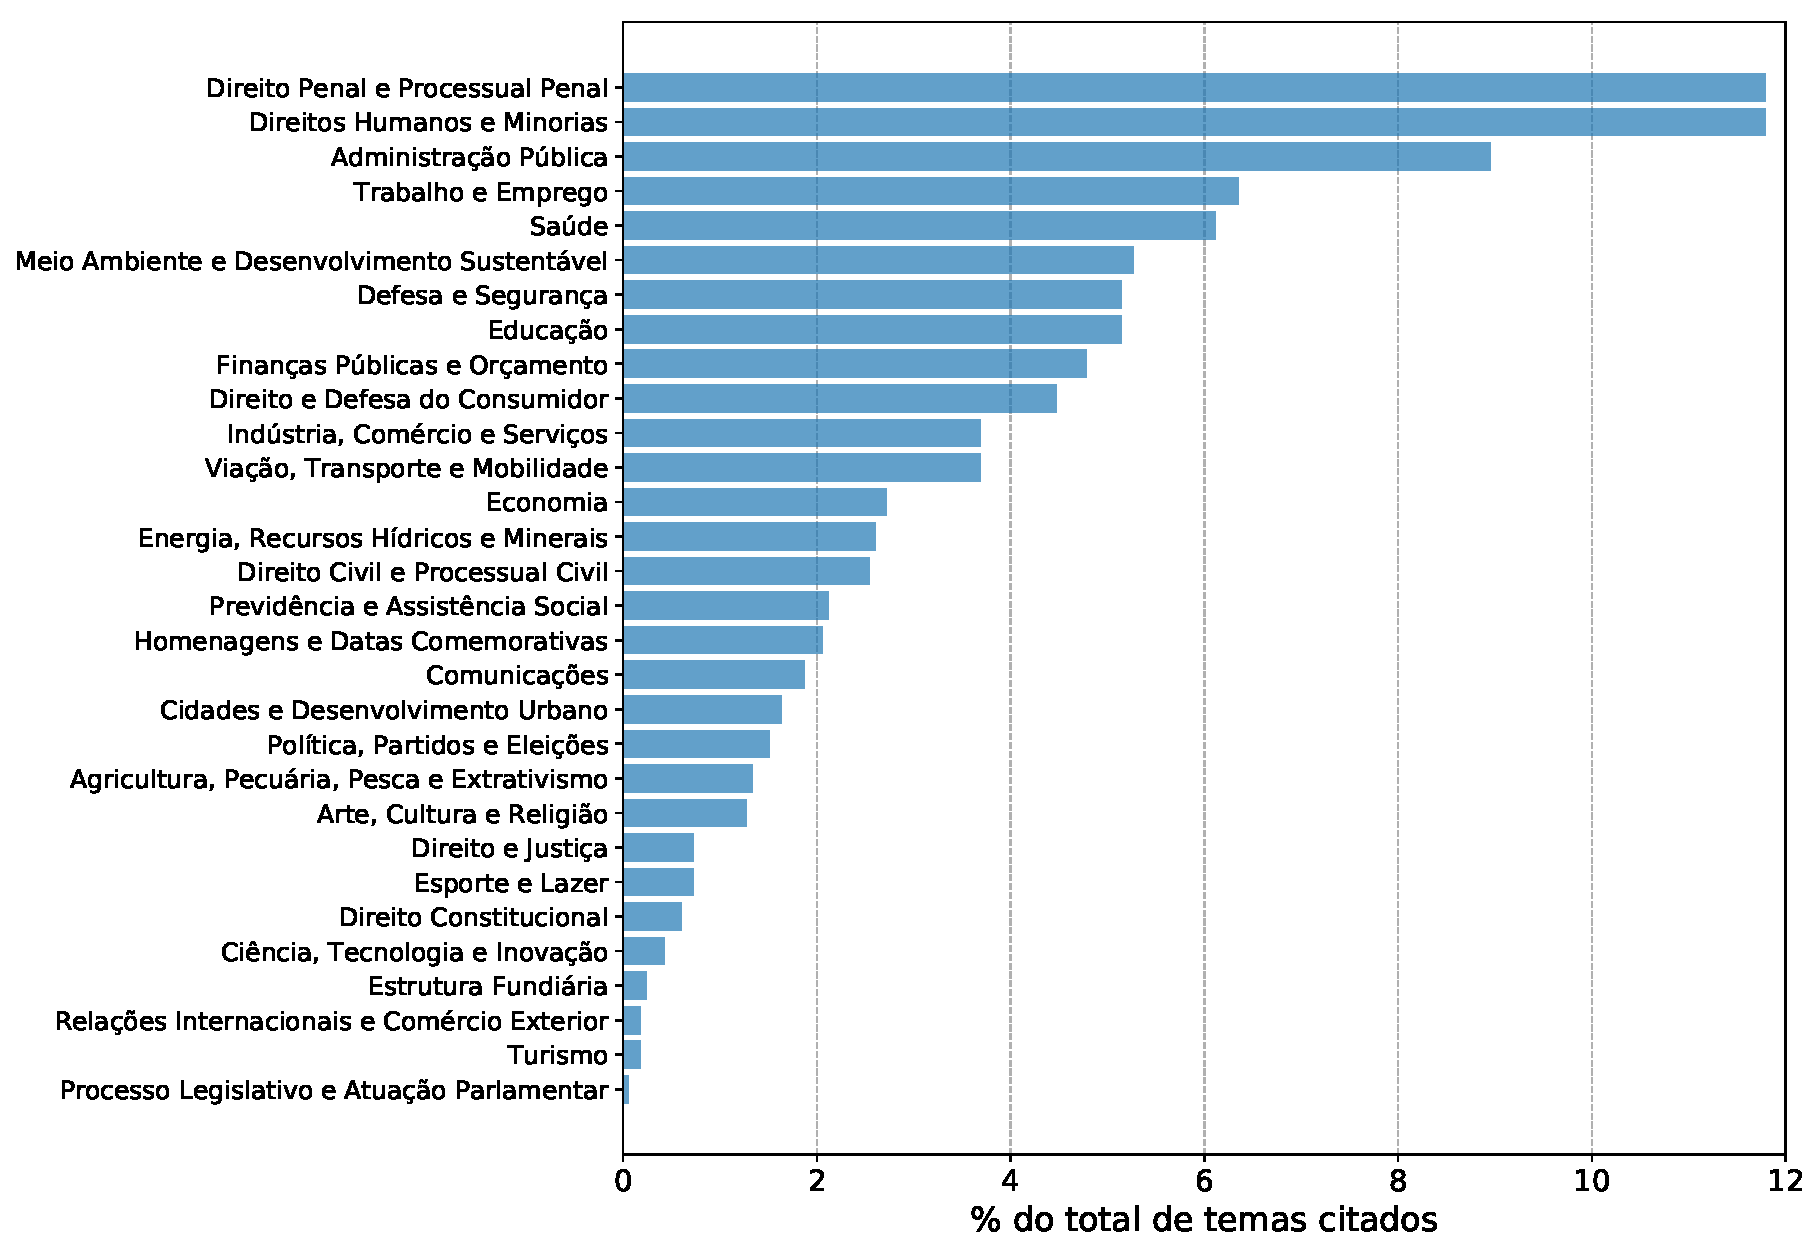
\includegraphics[width=1.0\textwidth]{graficos/temas_PL_fracao2019_2019-05-03.pdf}
\caption{Versão simplificada da Fig. \ref{fig:pl-por-tema-camara}. Aqui apenas apresentamos a frequência com
  que os temas apareceram na câmara nos 100 primeiros dias de 2019, sem comparar com o histórico.}
\label{fig:pl-por-tema-camara-simples}
\end{figure}

\begin{figure}[H]
\centering
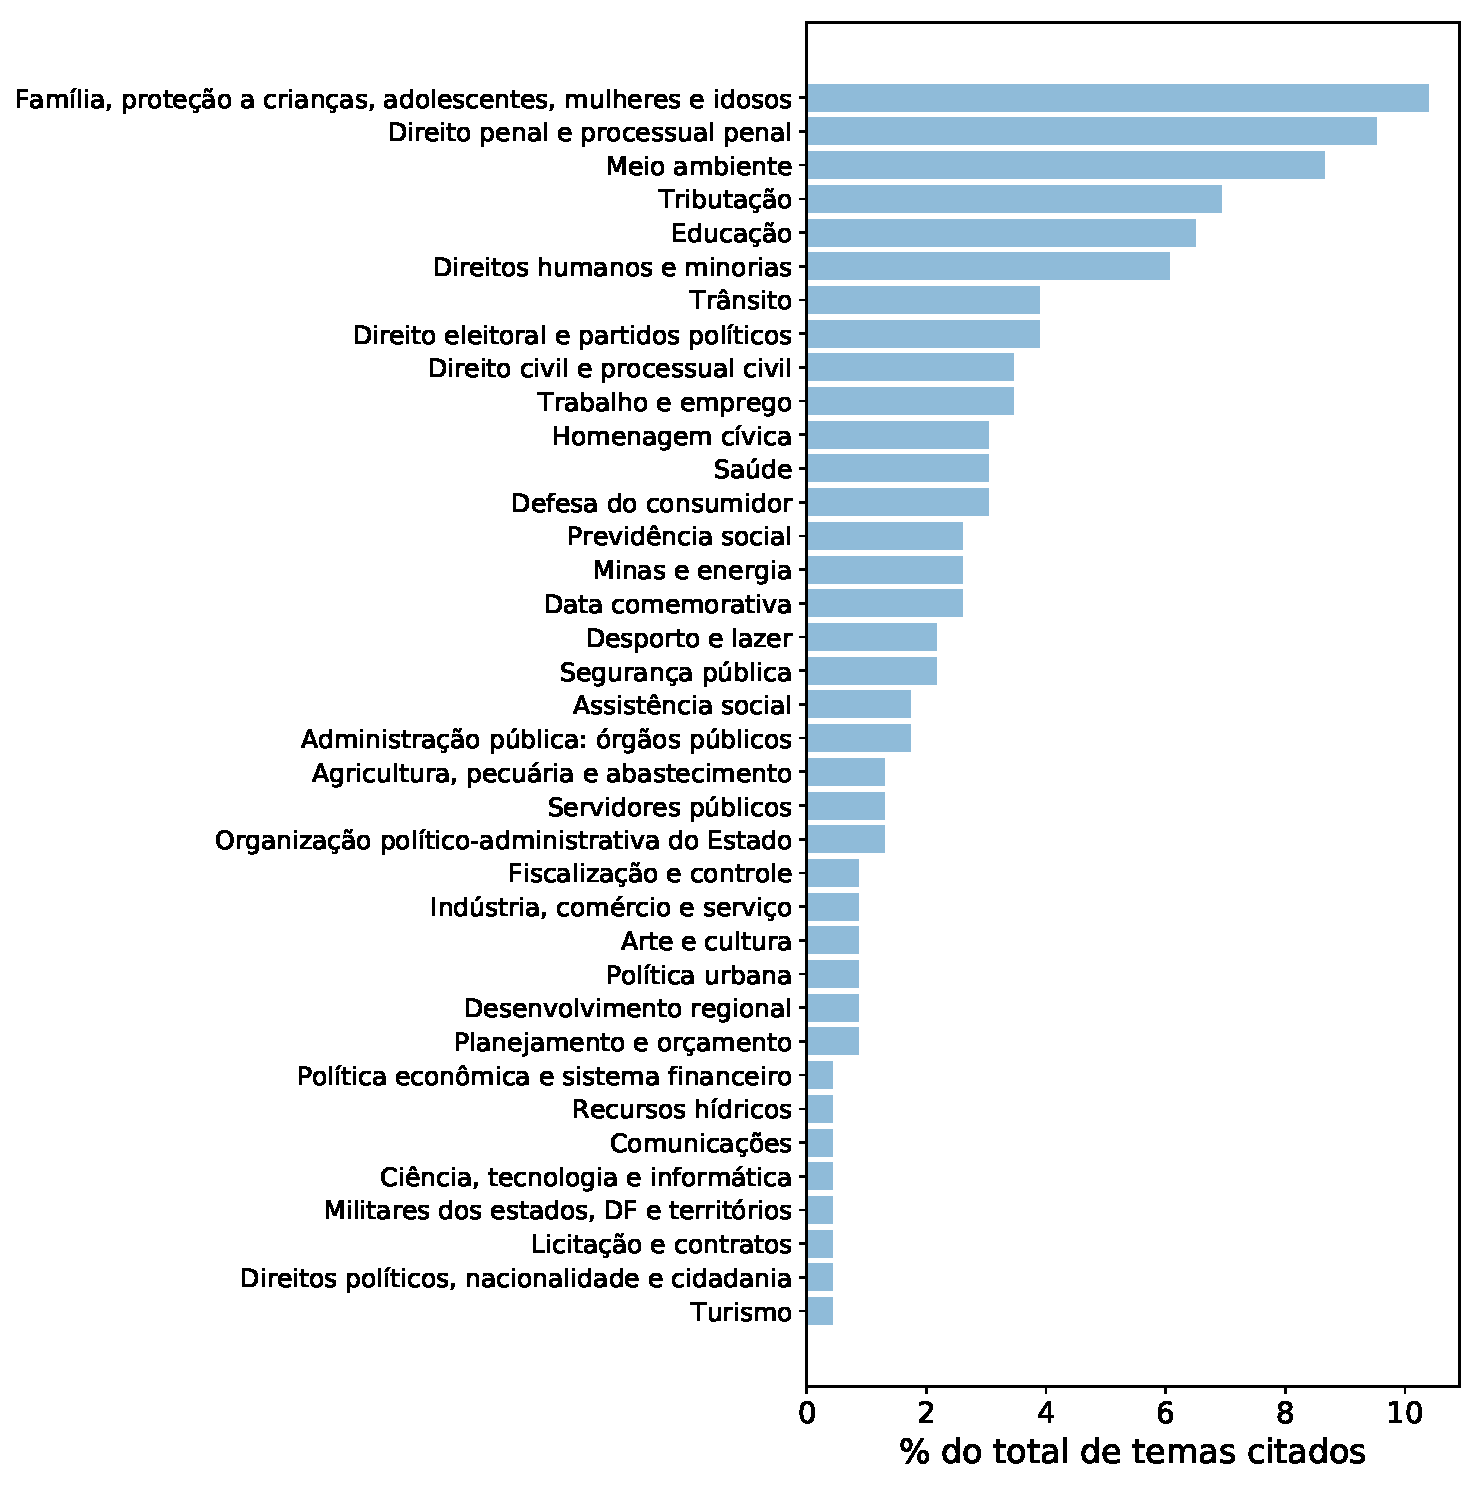
\includegraphics[width=1.0\textwidth]{graficos/senado/pls-temas-senado-r-simples.pdf}
\caption{Versão simplificada da Fig. \ref{fig:pl-por-tema-senado}. Aqui apenas apresentamos a frequência com
  que os temas apareceram no senado nos 100 primeiros dias de 2019, sem comparar com o histórico.}
\label{fig:pl-por-tema-senado-simples}
\end{figure}


\end{document}
